% !TeX spellcheck = sp
\documentclass[a4paper,11pt]{book}
%\documentclass[a4paper,twoside,11pt,titlepage]{book}
\usepackage[utf8]{inputenc}
\usepackage[spanish]{babel}
\usepackage{tikz}
\usepackage{tikz-cd}
\usetikzlibrary{babel}
%\usepackage[round]{natbib}
\usepackage[backend=bibtex,citestyle=alphabetic]{biblatex}
\addbibresource{bibliography/bibliography.bib}
\usepackage{float}
\usepackage{tikz-3dplot}
\usepackage[toc,page]{appendix}
\usetikzlibrary{patterns}
\usetikzlibrary{calc}
\usepackage{pgfplots}
\usetikzlibrary{external}
\usepackage{amsmath,amsthm,amssymb}
\usepackage{caption}
\usepackage{subcaption}

\usepackage{hyperref}
\usepackage{xcolor}

\hypersetup{
    colorlinks,
    citecolor=black,
    filecolor=black,
    linkcolor=black,
    urlcolor=black
}

\setlength{\parindent}{2em}
\setlength{\parskip}{0.4em}
\renewcommand{\baselinestretch}{1.0}
\setlength{\textfloatsep}{5pt}

\usepackage{minted}
\definecolor{monokaibg}{HTML}{272822}
\definecolor{friendlybg}{HTML}{f0f0f0}

% \usepackage[style=list, number=none]{glossary} %
%\usepackage{titlesec}
%\usepackage{pailatino}

\graphicspath{{img/}}
\decimalpoint
\usepackage{dcolumn}
\newcolumntype{.}{D{.}{\esperiod}{-1}}
\makeatletter
\addto\shorthandsspanish{\let\esperiod\es@period@code}
\makeatother


%\usepackage[chapter]{algorithm}
\RequirePackage{verbatim}
%\RequirePackage[Glenn]{fncychap}
\usepackage{fancyhdr}
\usepackage{graphicx}
\usepackage{afterpage}

\usepackage{longtable}
 
% ********************************************************************
% Re-usable information
% ********************************************************************
\newcommand{\myTitle}{P2-Navarro-Ramírez-Pilar.pdf\xspace}
\newcommand{\myDegree}{Grado en Ingeniería Informática y Matemáticas\xspace}
\newcommand{\myName}{Pilar Navarro Ramírez\xspace}
%\newcommand{\myProf}{M. Jesús García-Ligero Ramírez\xspace}
%\newcommand{\myOtherProf}{Carlos Ureña Almagro\xspace}
\newcommand{\myFaculty}{Escuela Técnica Superior de Ingenierías Informática y de
Telecomunicación\xspace}
\newcommand{\myFacultyShort}{E.T.S. de Ingenierías Informática y de
Telecomunicación\xspace}
\newcommand{\myUni}{\protect{Universidad de Granada}\xspace}
\newcommand{\myLocation}{Granada\xspace}
\newcommand{\myTime}{\today\xspace}
\newcommand{\myVersion}{Version 0.1\xspace}

\hypersetup{
pdfauthor = {\myName antoniogamiz10@gmail.com},
pdftitle = {\myTitle},
pdfsubject = {},
pdfkeywords = {raytracing, montecarlo, random, numbers},
pdfcreator = {pdflatex},
pdfproducer = {pdflatex}
}

%\hyphenation{}


%\usepackage{doxygen/doxygen}
\usepackage{url}
\usepackage{colortbl,longtable}
\usepackage[stable]{footmisc}
%\usepackage{index}

%\makeindex
%\usepackage[style=long, cols=2,border=plain,toc=true,number=none]{glossary}
% \makeglossary

% Definición de comandos que me son tiles:
%\renewcommand{\indexname}{Índice alfabético}
%\renewcommand{\glossaryname}{Glosario}

\pagestyle{fancy}
\fancyhf{}
\fancyhead[LO]{\leftmark}
\fancyhead[RE]{\rightmark}
\fancyhead[RO,LE]{\textbf{\thepage}}
%\renewcommand{\chaptermark}[1]{\markboth{\textbf{#1}}{}}
%\renewcommand{\sectionmark}[1]{\markright{\textbf{\thesection. #1}}}

\setlength{\headheight}{1.5\headheight}

\newcommand{\HRule}{\rule{\linewidth}{0.5mm}}
%Definimos los tipos teorema, ejemplo y definición podremos usar estos tipos
%simplemente poniendo \begin{teorema} \end{teorema} ...
%\newtheorem{theorem}{Teorema}[chapter]
%\newtheorem{example}{Ejemplo}[chapter]
%\newtheorem{definition}[chapter]{Definición}

\newcommand{\bigrule}{\titlerule[0.5mm]}


%Para conseguir que en las páginas en blanco no ponga cabecerass
\makeatletter
\def\clearpage{%
  \ifvmode
    \ifnum \@dbltopnum =\m@ne
      \ifdim \pagetotal <\topskip
        \hbox{}
      \fi
    \fi
  \fi
  \newpage
  \thispagestyle{empty}
  \write\m@ne{}
  \vbox{}
  \penalty -\@Mi
}
\makeatother

\usepackage{pdfpages}

\usepackage[a4paper, margin={1in}]{geometry}

\begin{document}

\begin{titlepage}
 
 
\newlength{\centeroffset}
\setlength{\centeroffset}{-0.5\oddsidemargin}
\addtolength{\centeroffset}{0.5\evensidemargin}
\thispagestyle{empty}

\noindent\hspace*{\centeroffset}\begin{minipage}{\textwidth}

\centering

\includegraphics[width=0.9\textwidth]{img/logo_ugr.jpg}\\[2cm]

\textsc{ \Huge Inteligencia de Negocio\\[1.5cm]}
\textbf{\textsc{ \huge Práctica 3:}}\\
 \huge  Competición en Kaggle\\[1cm]
% Upper part of the page
% 
% Title
%{\Huge\bfseries \\
%}
%\noindent\rule[-1ex]{\textwidth}{3pt}\\[3.5ex]
%{\large\bfseries }
\end{minipage}

\vspace{2cm}
\noindent\hspace*{\centeroffset}\begin{minipage}{\textwidth}
\centering

\textbf{Autor}\\[0.2cm] {Pilar Navarro Ramírez}\\[0.2cm]
pilarnavarro@correo.ugr.es \\[0.2cm]
Grupo de prácticas 1 \\[1cm]


\includegraphics[width=0.3\textwidth]{img/etsiit_logo.png}\\[0.1cm]
\textsc{Escuela Técnica Superior de Ingeniería Informática y de Telecomunicaciones}\\
\textsc{---}\\
Granada, 4 de enero de 2021
\end{minipage}
%\addtolength{\textwidth}{\centeroffset}
%\vspace{\stretch{2}}
\end{titlepage}



%\input{preface/preface}

%\tableofcontents
%\listoffigures
%\listoftables

\tableofcontents
\newpage

\chapter{Apartado 1: Visualización}
\section{Visualización de las medidas}

Vamos a mostrar, haciendo uso de diagramas de barras, los resultados obtenidos de las medidas de Accuracy, AUC y F1-Score en cada uno de los preprocesamientos y para cada uno de los clasificadores usados en la práctica anterior:
\begin{center}
	\begin{figure}[H]
		\centering
		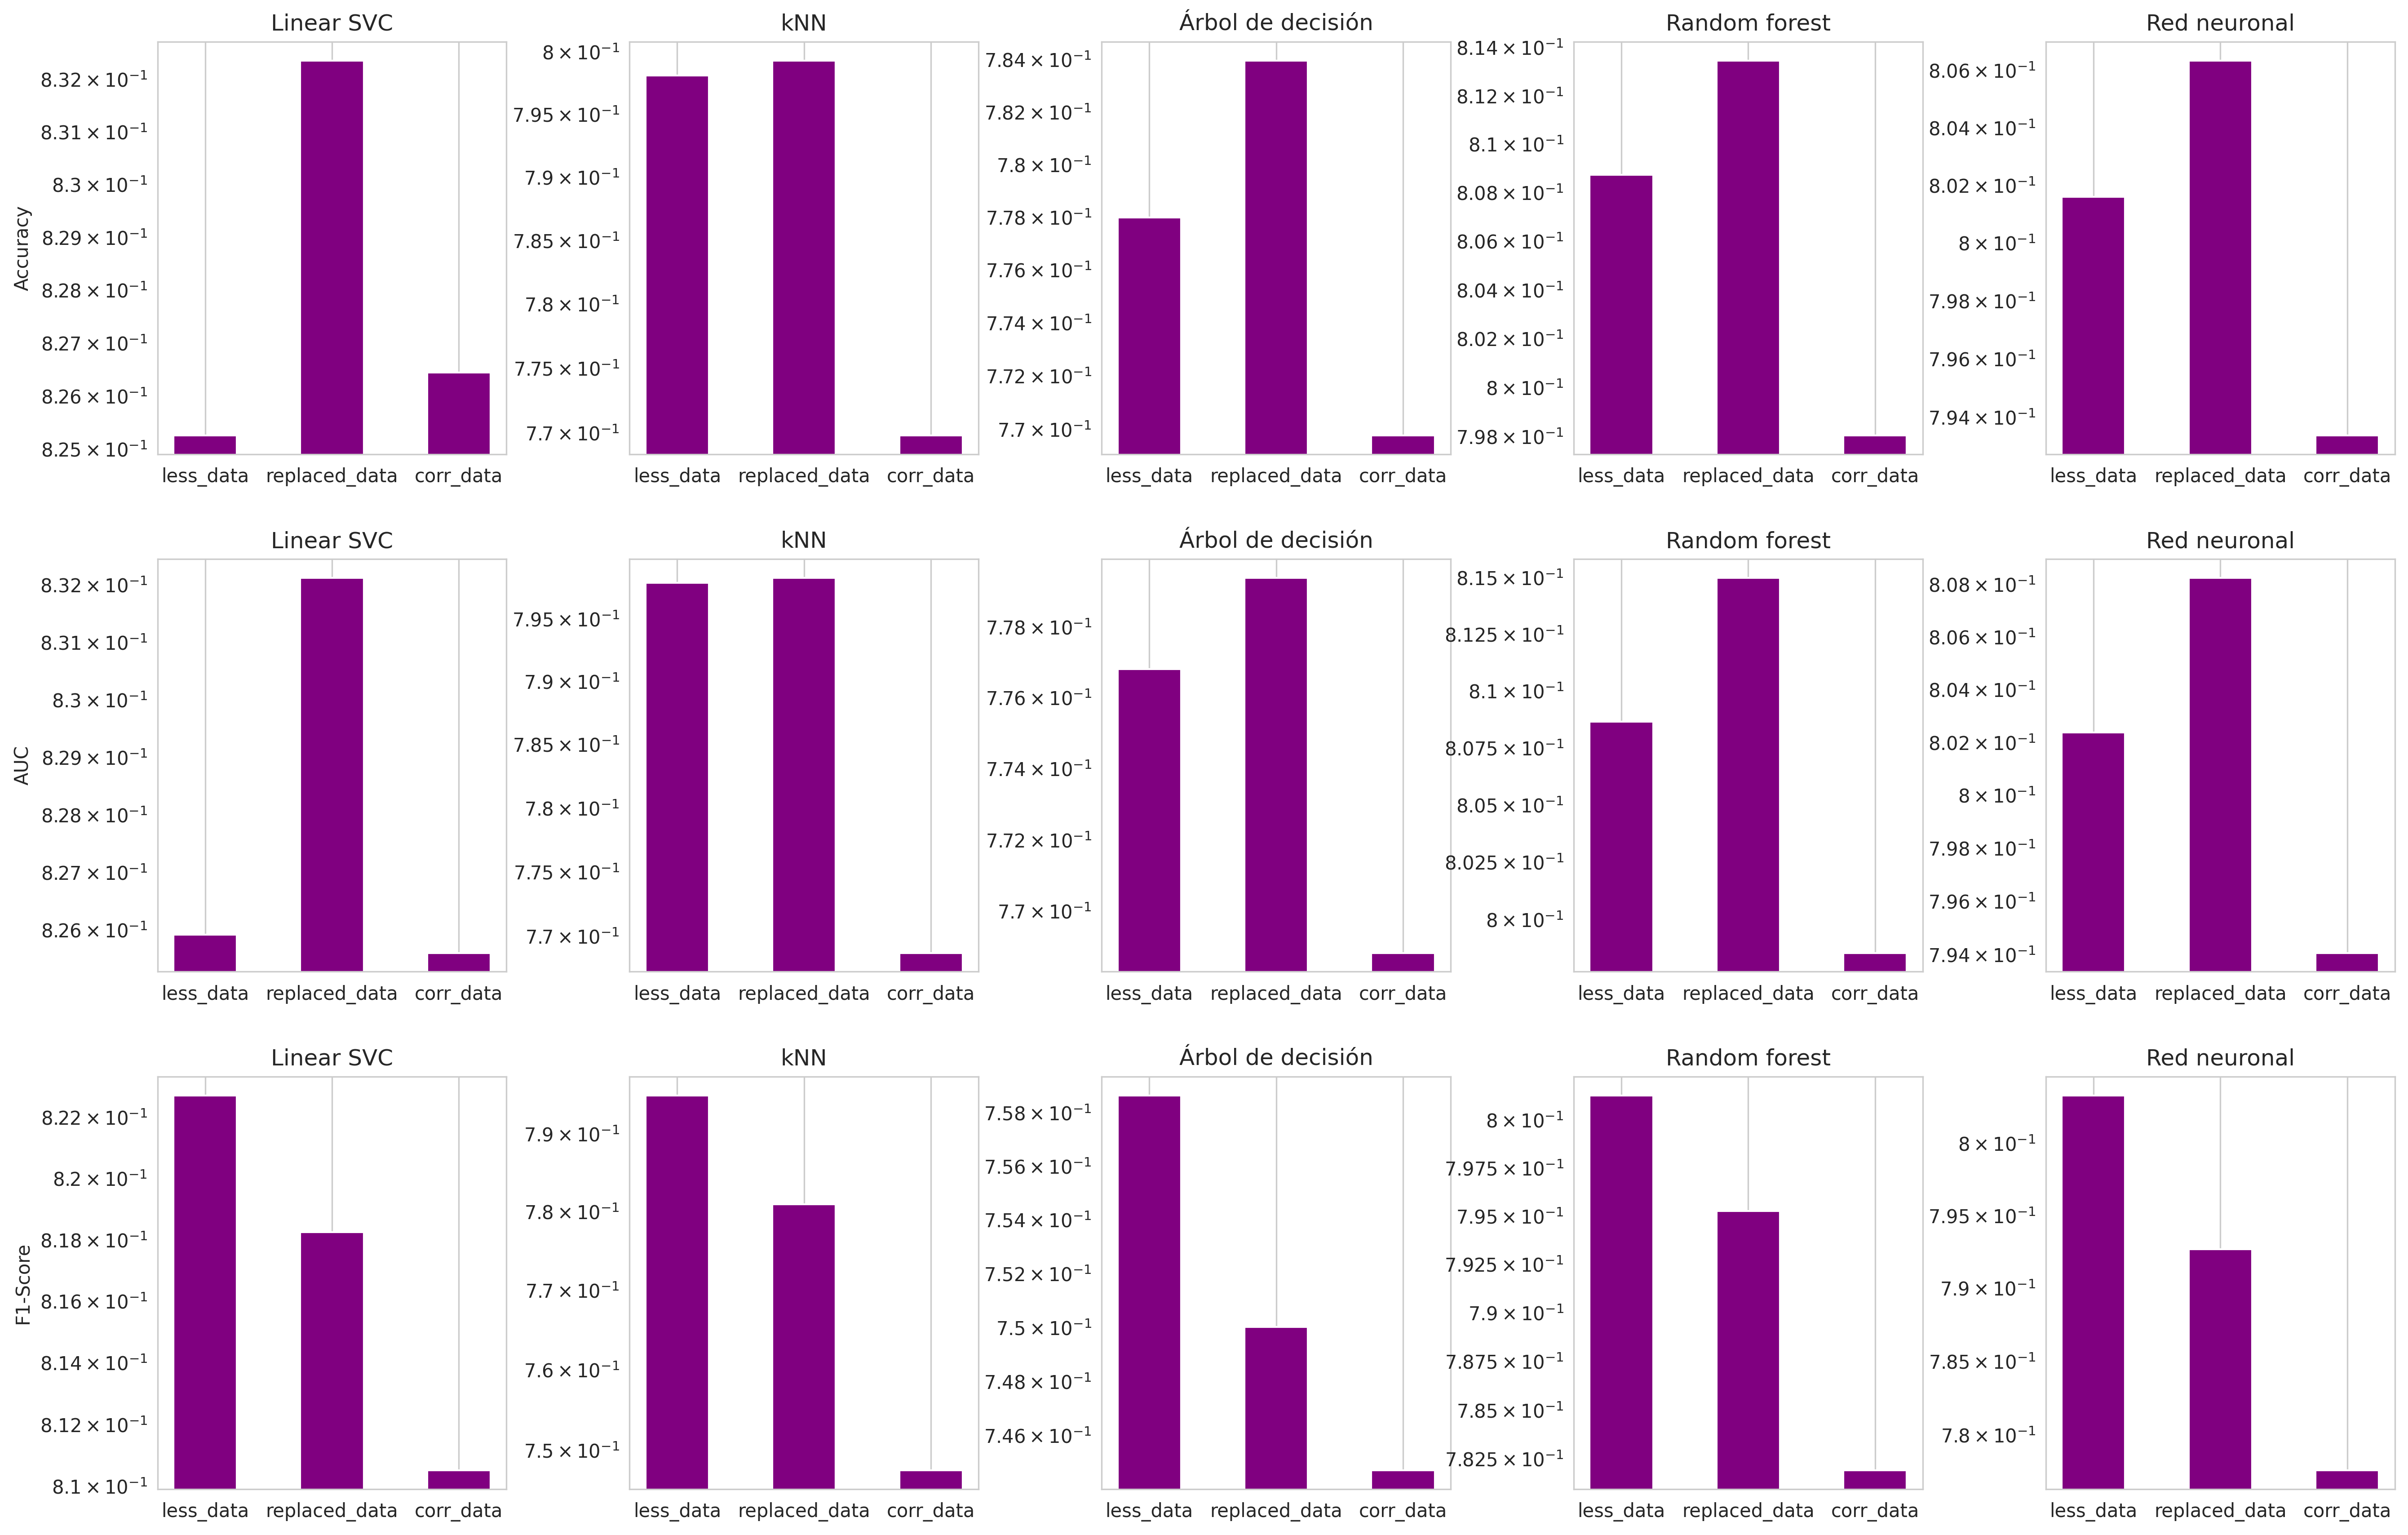
\includegraphics[width=1.1\linewidth]{img/preprocesamiento}
		\caption{}
		\label{fig:preprocesamiento}
	\end{figure}
\end{center}

podemos observar que los datos preprocesados \mintinline{python}{replaced_data}, en los que reemplazamos los valores perdidos por el valor más frecuente de la columna correspondiente, nos ofrecen los mejores resultados del Acurracy y AUC para todos los clasificadores estudiados, mientras que los datos \mintinline{python}{less_data}, en los que simplemente eliminamos todas las instancias con valores perdidos, presentan los mejores valores del F1-Score en todos los clasificadores. Por su parte \mintinline{python}{corr_data} ofrece resultados muy bajos para todas las medidas consideradas y todos los modelos, con lo que este es el peor de todos los procesamientos realizados.

Otro detalle que podemos notar es que la diferencia entre los resultados de los preprocesamientos \mintinline{python}{replaced_data} y  \mintinline{python}{less_data} en el algoritmo de K-nn es muy pequeña. Para Linear SVC, la diferencia entre dichos preprocesamientos para las medidas de Accuracy y AUC es muy grande, presentando los datos  \mintinline{python}{replaced_data} los mejores resultados. Para el resto de clasificadores y medidas, las diferencias entre \mintinline{python}{replaced_data} y \mintinline{python}{less_data} son muy similares. Además, la diferencia entre ambos preprocesamientos y \mintinline{python}{corr_data} es muy elevada, siendo este último preprocesamiento el peor con diferencia. 

Para llevar a cabo esta visualización hemos usado unos ficheros \mintinline{python}{.csv} (\mintinline{python}{accuracy.csv}, \mintinline{python}{auc.csv}, \mintinline{python}{f1.csv}) en los que hemos almacenado los resultados de cada una de las medidas consideradas que obtuvimos en la práctica anterior para cada preprocesamiento y cada modelo. 

\section{Gráficas de curva ROC}

Si visualizamos la curva ROC de cada uno de los modelos estudiados en la práctica anterior, entrenados sobre el conjunto de datos \mintinline{python}{less_data} y con la configuración de parámetros que nos dio los mejores resultados, obtenemos lo siguiente:
\begin{figure}[H]
	\centering
	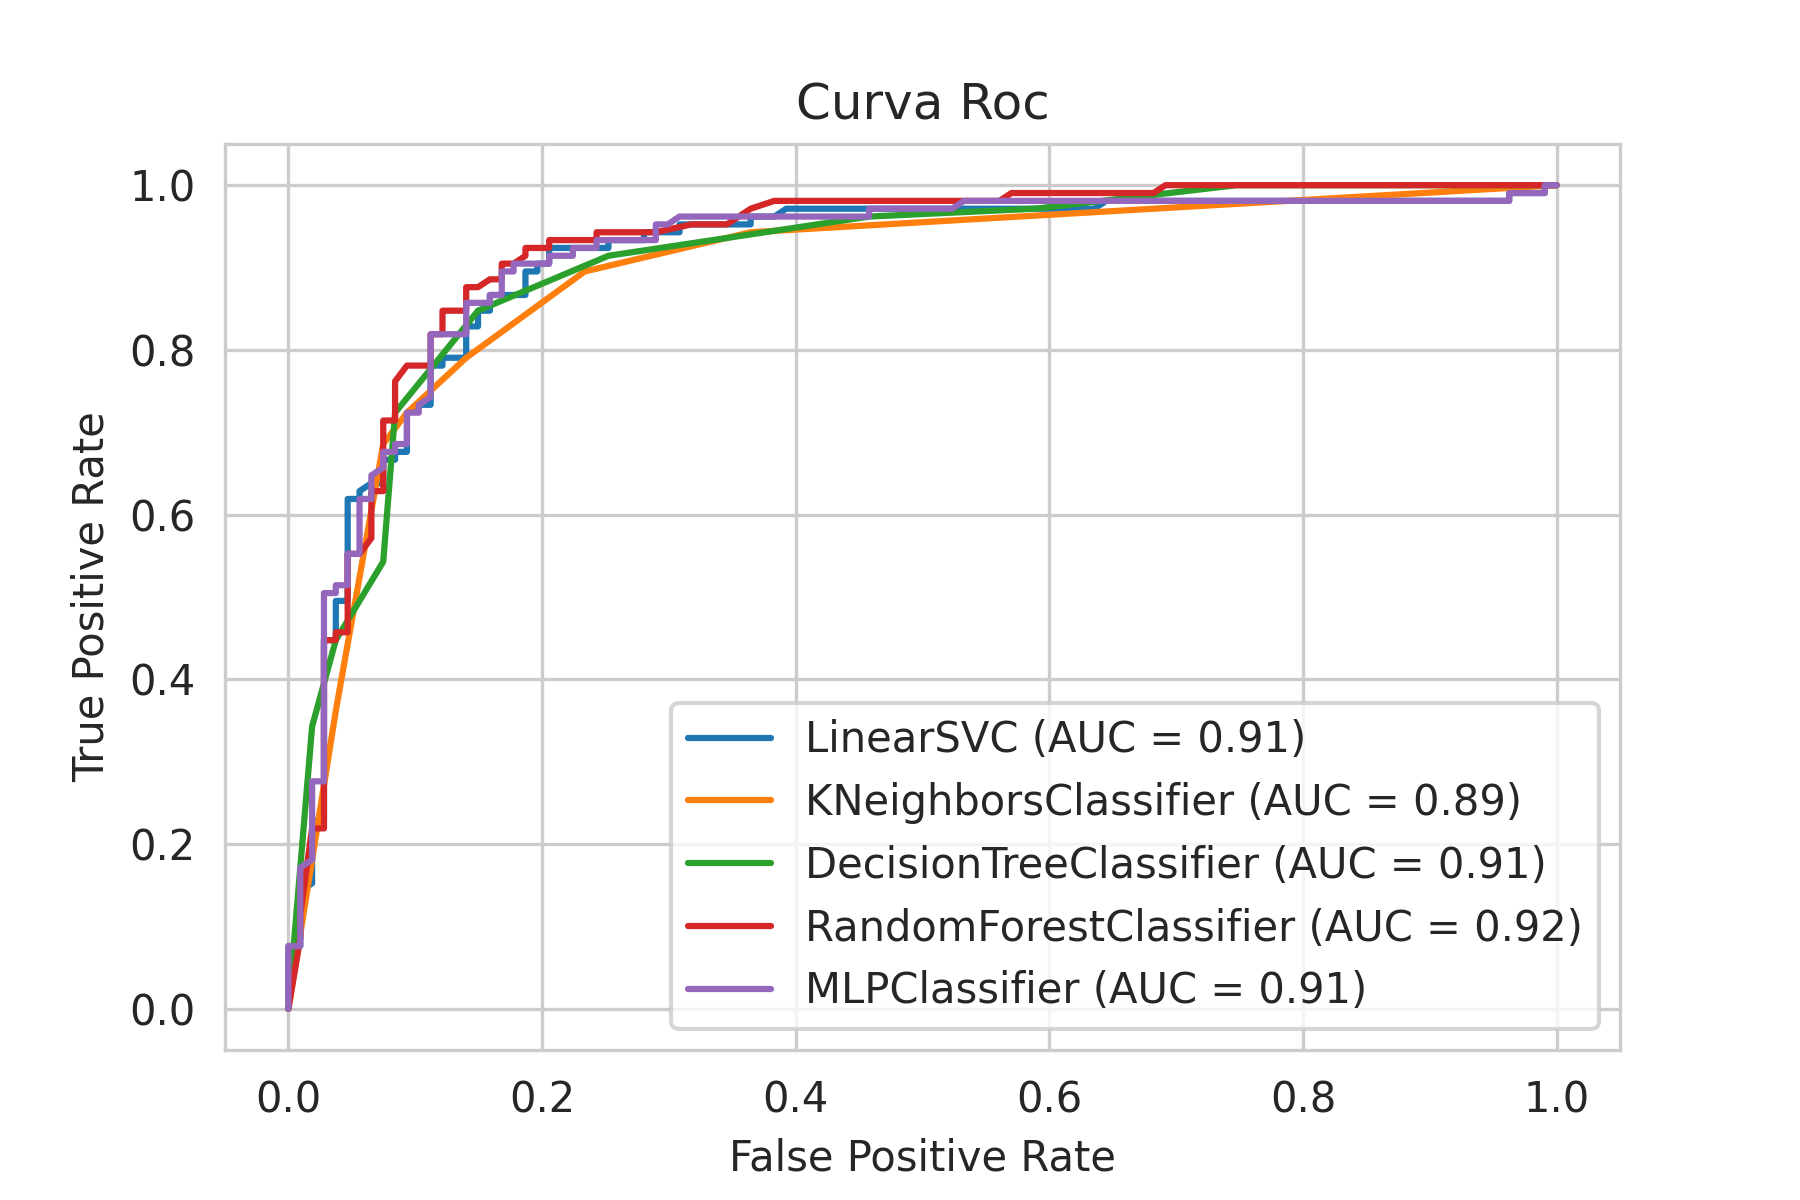
\includegraphics[width=0.9\linewidth]{img/curva_roc}
	\caption{}
	\label{fig:curvaroc}
\end{figure}

Nos damos cuenta entonces de que el modelo que presenta los mejores resultados según el AUC y su respectiva curva ROC es el Random Forest, seguido por las redes neuronales, la máquina de soporte vectorial lineal y los árboles de decisión, siendo el algoritmo del vecino más cercano el que ofrece un valor más bajo de AUC y presenta una peor curva ROC. 

\newpage
\section{Análisis de los atributos}

En este apartado llevamos a cabo un análisis de los atributos del dataset de mamografías, intentando buscar relaciones entre los distintos atributos y la importancia de los mismos en la determinación de la severidad del tumor. Para ello, realizamos distintas visualizaciones que muestren la relación de dichos atributos con el atributo \textit{severidad}. 

Empezamos viendo los diagramas de cajas que relacionan cada una de las variables con el tipo de tumor:

\begin{figure}[H]
	\centering
	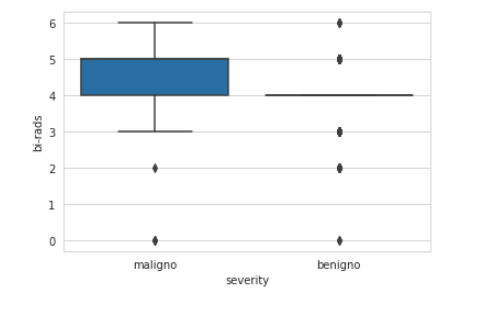
\includegraphics[width=0.8\linewidth]{img/box1}
	\caption{}
	\label{fig:box1}
\end{figure}
\begin{figure}[H]
	\centering
	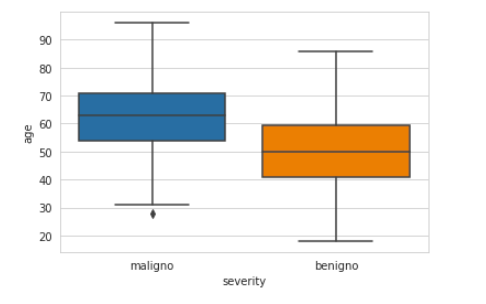
\includegraphics[width=0.8\linewidth]{img/box2}
	\caption{}
	\label{fig:box2}
\end{figure}
\begin{figure}[H]
	\centering
	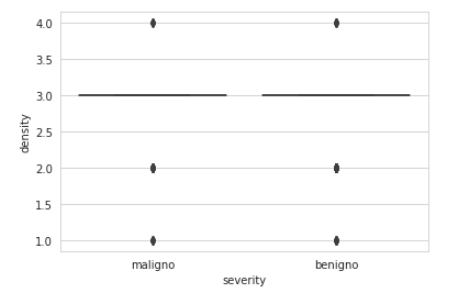
\includegraphics[width=0.8\linewidth]{img/box3}
	\caption{}
	\label{fig:box3}
\end{figure}
\begin{figure}[H]
	\centering
	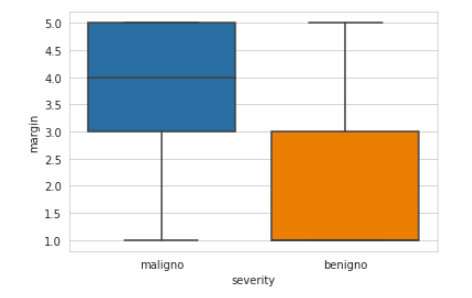
\includegraphics[width=0.8\linewidth]{img/box4}
	\caption{}
	\label{fig:box4}
\end{figure}
\begin{figure}[H]
	\centering
	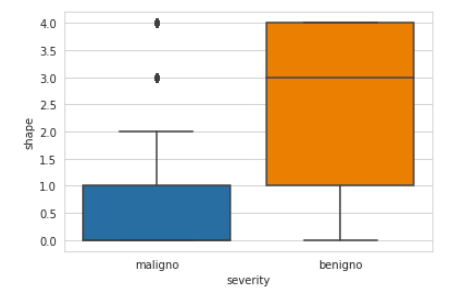
\includegraphics[width=0.6\linewidth]{img/box5}
	\caption{}
	\label{fig:box5}
\end{figure}
Vemos además la relación de cada uno de los atributos con los demás usando una imagen \mintinline{python}{pairplot}, donde cada uno de los datos ha sido etiquetado con la severidad del tumor que tiene asociado:
\begin{figure}[H]
	\centering
	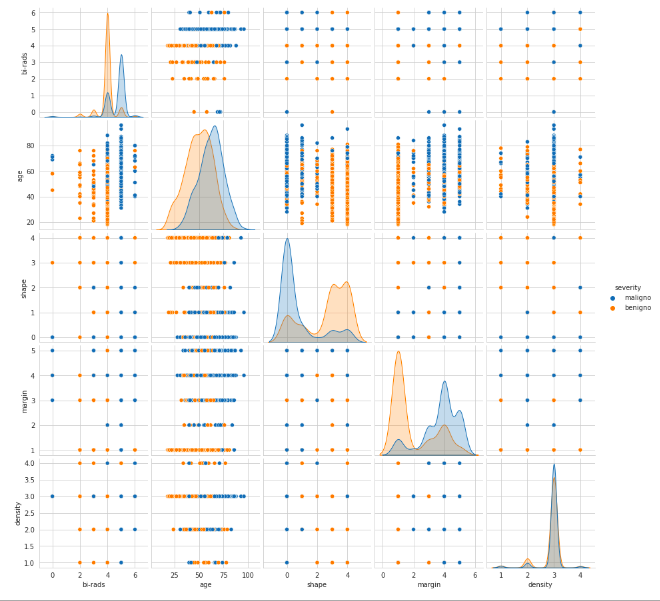
\includegraphics[width=1\linewidth]{img/pairplotatributos}
	\caption{}
	\label{fig:pairplotatributos}
\end{figure}

Ahora mostramos unos diagramas de barras en los que, para cada valor de un atributo concreto, se muestra el número de instancias que hay en el conjunto de datos etiquetadas con cada uno de los tipos de tumor:
\begin{figure}[H]
	\centering
	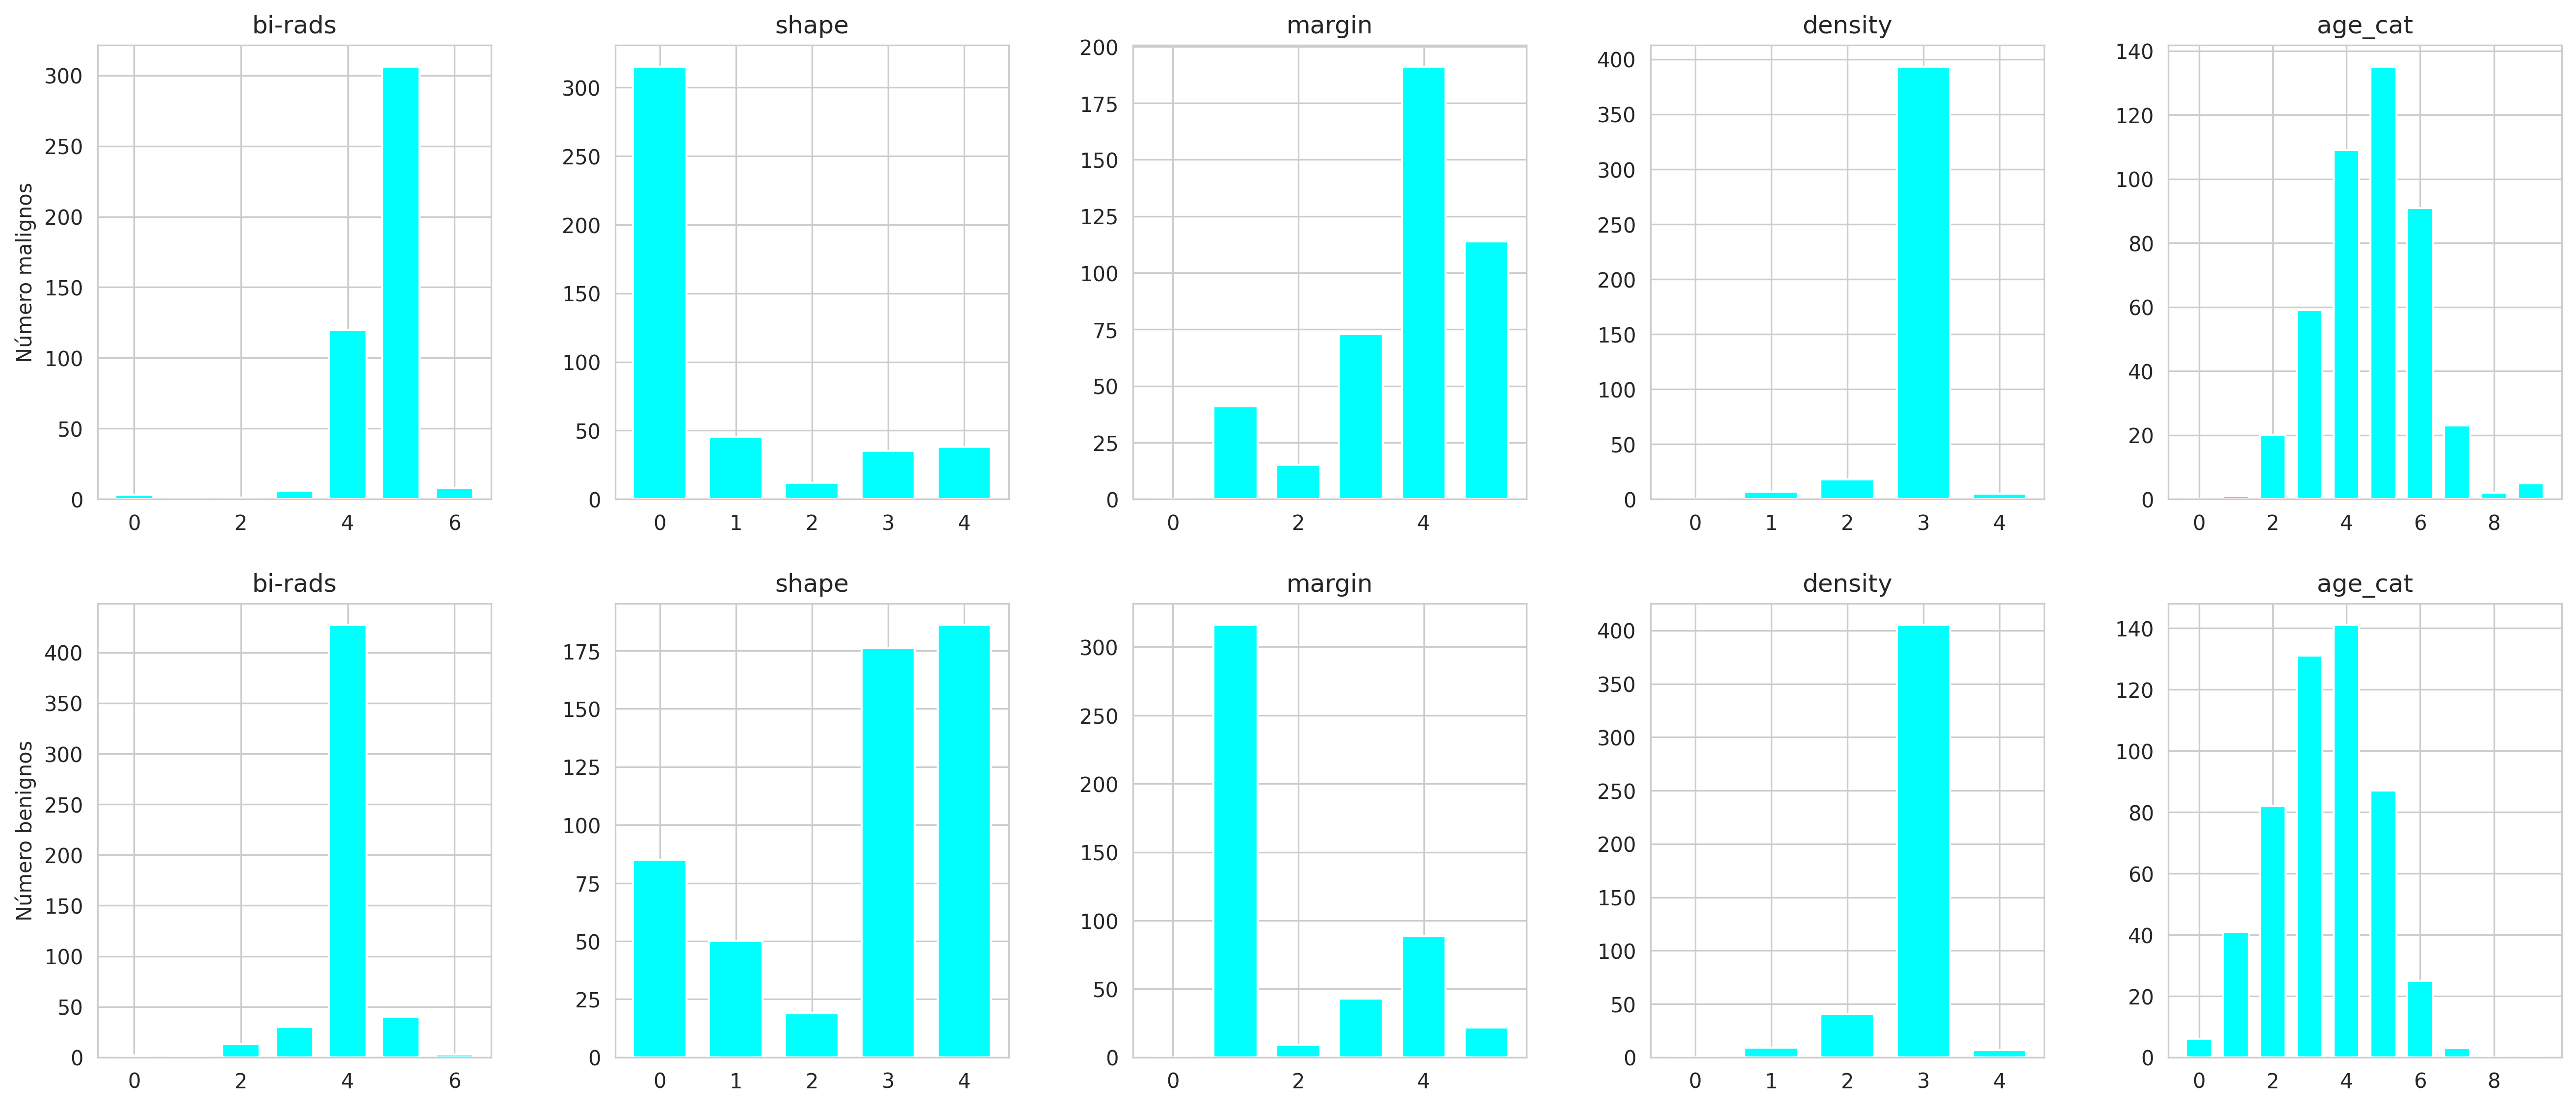
\includegraphics[width=1.1\linewidth]{img/analisis}
	\caption{}
	\label{fig:analisis}
\end{figure}
Los atributos nominales han sido convertidos a numéricos, de manera que cada valor de la variable tiene asociado un número. La edad ha sido tratada de forma especial para poder llevar a cabo esta visualización: hemos considerado rangos de edades ("0-20", "20-30", "30-40", "40-50","50-60","60-70","70-80", "80-90","90-100") y hemos asignado a cada instancia el valor que le correpondía; a continuación, estos rangos de edades, considerados como valores nominales, han sido transformados a valores numéricos de la misma forma que el resto de atributos categóricos, con lo que a cada uno de estos rangos se le ha asignado un número entre 0 y 8 de forma ordenada.

A la vista de estos gráficos, podemos ahora analizar los atributos como comentamos al principio de la sección. 

El primer aspecto del que nos damos cuenta es que el atributo \underline{density} no tiene ninguna relación con el tipo de tumor, pues observando el diagrama de cajas vemos que para ambos valores del atributo severidad, el atributo density presenta una distribución degenerada en 3, sin tener en cuenta los outliers, es decir, en casi todos los datos, independientemente de si están etiquetados como cáncer maligno o benigno, este atributo toma el valor 3. A la misma conclusión podemos llegar observando los diagramas de barras o la imagen pairplot, pues las gráficas de densidad del atributo density se solapan, esto es, la distribución de este atributo es exactamente la misma para los dos valores de la variable severity. 

Algo parecido ocurre con el atributo de \underline{edad}. Aunque en este caso no está tan claro, podemos observar que sus correspondientes gráficas de densidad también están casi solapadas. Fijándonos en los diagramas de barras de la edad, vemos también que el diagrama cambia solo un poco para los diferentes valores de la severidad, sobre todo para el rango de edades 30-40 y 50-60 años, pues el número de tumores benignos es mayor en estos rangos que el número de tumores malignos. Por lo tanto, podemos decir que el atributo de edad aporta algo más de información que el anterior, aunque dicha información tampoco es muy relevante o determinante para el tipo de tumor. 

El resto de atributos sí tienen mayor relación con la severidad del tumor. Prestando atención a los diagramas de barras vemos que el atributo \underline{margin} es bastante informativo, pues casi todos los tumores malignos presentan un valor alto de esta variable (3, 4 y 5), siendo el valor 4 el más frecuente entre este tipo de tumor. Por su parte, la mayoría de los tumores benignos tienen un valor de margin de 1. Fijándonos en la imagen pairplot observamos además que los gráficos de densidad de este atributo a penas se solapan, lo que de nuevo nos dice que este atributo diferencia bastante bien entre los dos tipos de tumores. Y lo mismo ocurre con las gráficas de densidad del atributo \underline{shape}, con lo que este también es informativo sobre la severidad del tumor. En los diagramas de barras de esta última variable observamos que la mayoría de los datos con cáncer maligno tienen un valor de shape de 0 y gran parte de los tumores benignos presentan una forma con valor 3 o 4. Por otro lado, centrándonos en los diagramas de cajas de estos dos atributos, podemos observar que los valores que toman el 75\% de los datos etiquetados con cada uno de los tipos de tumor son bastante diferentes para cada caso: el 75\% de los datos con severidad maligna presentan un valor de 0 ó 1 para el atributo shape y de entre 3 y 5 para margin, mientras que el 75\% de las instancias con tumor benigno tienen una forma de entre 1 y 4 y un margin de entre 1 y 3. 

Finalmente, nos queda analizar el \underline{atributo BI-RADS}. Los diagramas de barras asociados al mismo nos muestran que prácticamente todos los datos etiquetados con tumor benigno tienen un valor de 4 para dicho atributo y los etiquetados con cáncer maligno toman un valor de 4 o 5 en su mayoría, siendo este último valor el más frecuente. Basándonos en los diagramas de cajas, notamos que la distribución de los datos con severidad benigna asociada a nuestro atributo es degenerada en 4 si no consideramos los outliers, y para los datos con tumor maligno esta es más dispersa, presentando la mitad de las instancias un valor de 4 o 5. Así pues, en el caso en que este atributo tenga un valor distinto de 4 o 5, no permite distinguir entre ambos tipos de tumor. Si presenta un valor de 4, es más probable que el cáncer sea maligno, aunque la probabilidad de que sea benigno es también alta. Si la variable toma el valor 5, es casi seguro que se tratará de un cáncer maligno. Así pues, podemos decir que este atributo no es tan determinante como los dos anteriores para la severidad del tumor, pero también juega un papel importante y aporta información valiosa en la clasificación. 

En resumen, podemos considerar que el atributo density no aporta nada de información para la clasificación de los datos en distintos tipos de tumores y la edad es muy poco informativa. Los atributos de density y margin son los más determinantes en la clasificación, aunque la información que proporciona BI-RADS también es crucial en muchos casos. 
\chapter{Apartado 2: Segmentación}
\section{Introducción}

Se dispone de un conjunto de datos publicados por la DGT que contiene información de los accidentes de tráfico que se produjeron en España en el año 2013, incluyendo diferentes variables que caracterizan a cada uno de los accidentes, y se desea analizar dichos datos para comprender mejor las dinámicas en accidentes de tráfico en España.

En esta práctica vamos a seleccionar distintos subconjuntos de datos de este \textit{dataset} atendiendo a ciertas variables de interés  y llevaremos a cabo una segmetación  de los mismos en varios grupos con características similares, con el objetivo de encontrar relaciones que expliquen los tipos y la gravedad de los accidentes.

Para realizar esta segmentación haremos uso de diferentes algoritmos de clustering, entre ellos el algoritmo de \textbf{K-means}. Estudiaremos los clusters finales proporcionados por cada uno de los algoritmos mediante diversas visualizaciones tratando de interpretar cada uno de ellos y de encontrar relaciones de causalidad. También analizaremos los resultados de cada algoritmo para poder compararlos entre sí. 

\newpage
\section{Caso de estudio 1}
\subsection{Elección del caso de estudio}
Como primer caso de estudio, nos vamos a centrar en los accidentes que ocurrieron en los meses de julio, agosto y septiembre.
Es bien sabido que esta es la época del año cuando se producen más accidentes de tráfico y estos son de mayor gravedad. Este hecho es bastante lógico: es en verano durante las vacaciones cuando tiene lugar un mayor número de desplazamientos, pues la gente sale de su lugar de residencia para pasar sus vacaciones en otra zona, visitar a familiares, etc. En el mes de septiembre se produce la vuelta al trabajo y al lugar de residencia habitual, de manera que los desplazamientos en esta época también son bastante elevados, lo que propicia un aumento en el número de accidentes. 
Para ver cómo influye el mes en los accidentes hemos llevado  a cabo una visualización de los datos relativos a la gravedad del accidente de que disponemos en nuestro dataset (total de víctimas, total de heridos leves y graves y total de muertos) atendiendo a este atributo. El diagrama de cajas obtenido para la variable 'número total de víctimas' es el siguiente:
\begin{figure}[H]
	\centering
	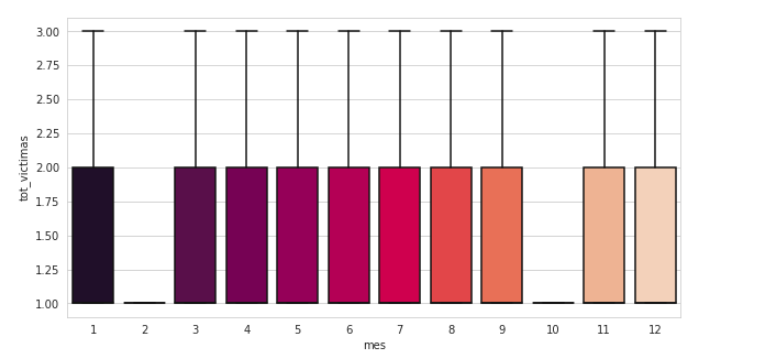
\includegraphics[width=1\linewidth]{img/cajas_mes}
	\caption{}
	\label{fig:cajasmes}
\end{figure}

En él podemos observar que no hay diferencias significativas en cuanto al tipo de distribución asociada a cada mes, salvo por los meses de febrero y octubre, en los que el número de víctimas máximo es 1. Hemos seleccionado el atributo 'número total de víctimas' para visualizar el diagrama de cajas porque engloba todos los tipos de víctimas implicadas en el accidente, por lo que es más representativo que el resto de atributos. 

Como apenas podemos sacar información de aquí, hemos realizado además la media del número total de víctimas, número total de heridos leves y graves y número total de muertos por cada mes y la hemos representado en un diagrama de barras:
\begin{figure}[H]
	\centering
	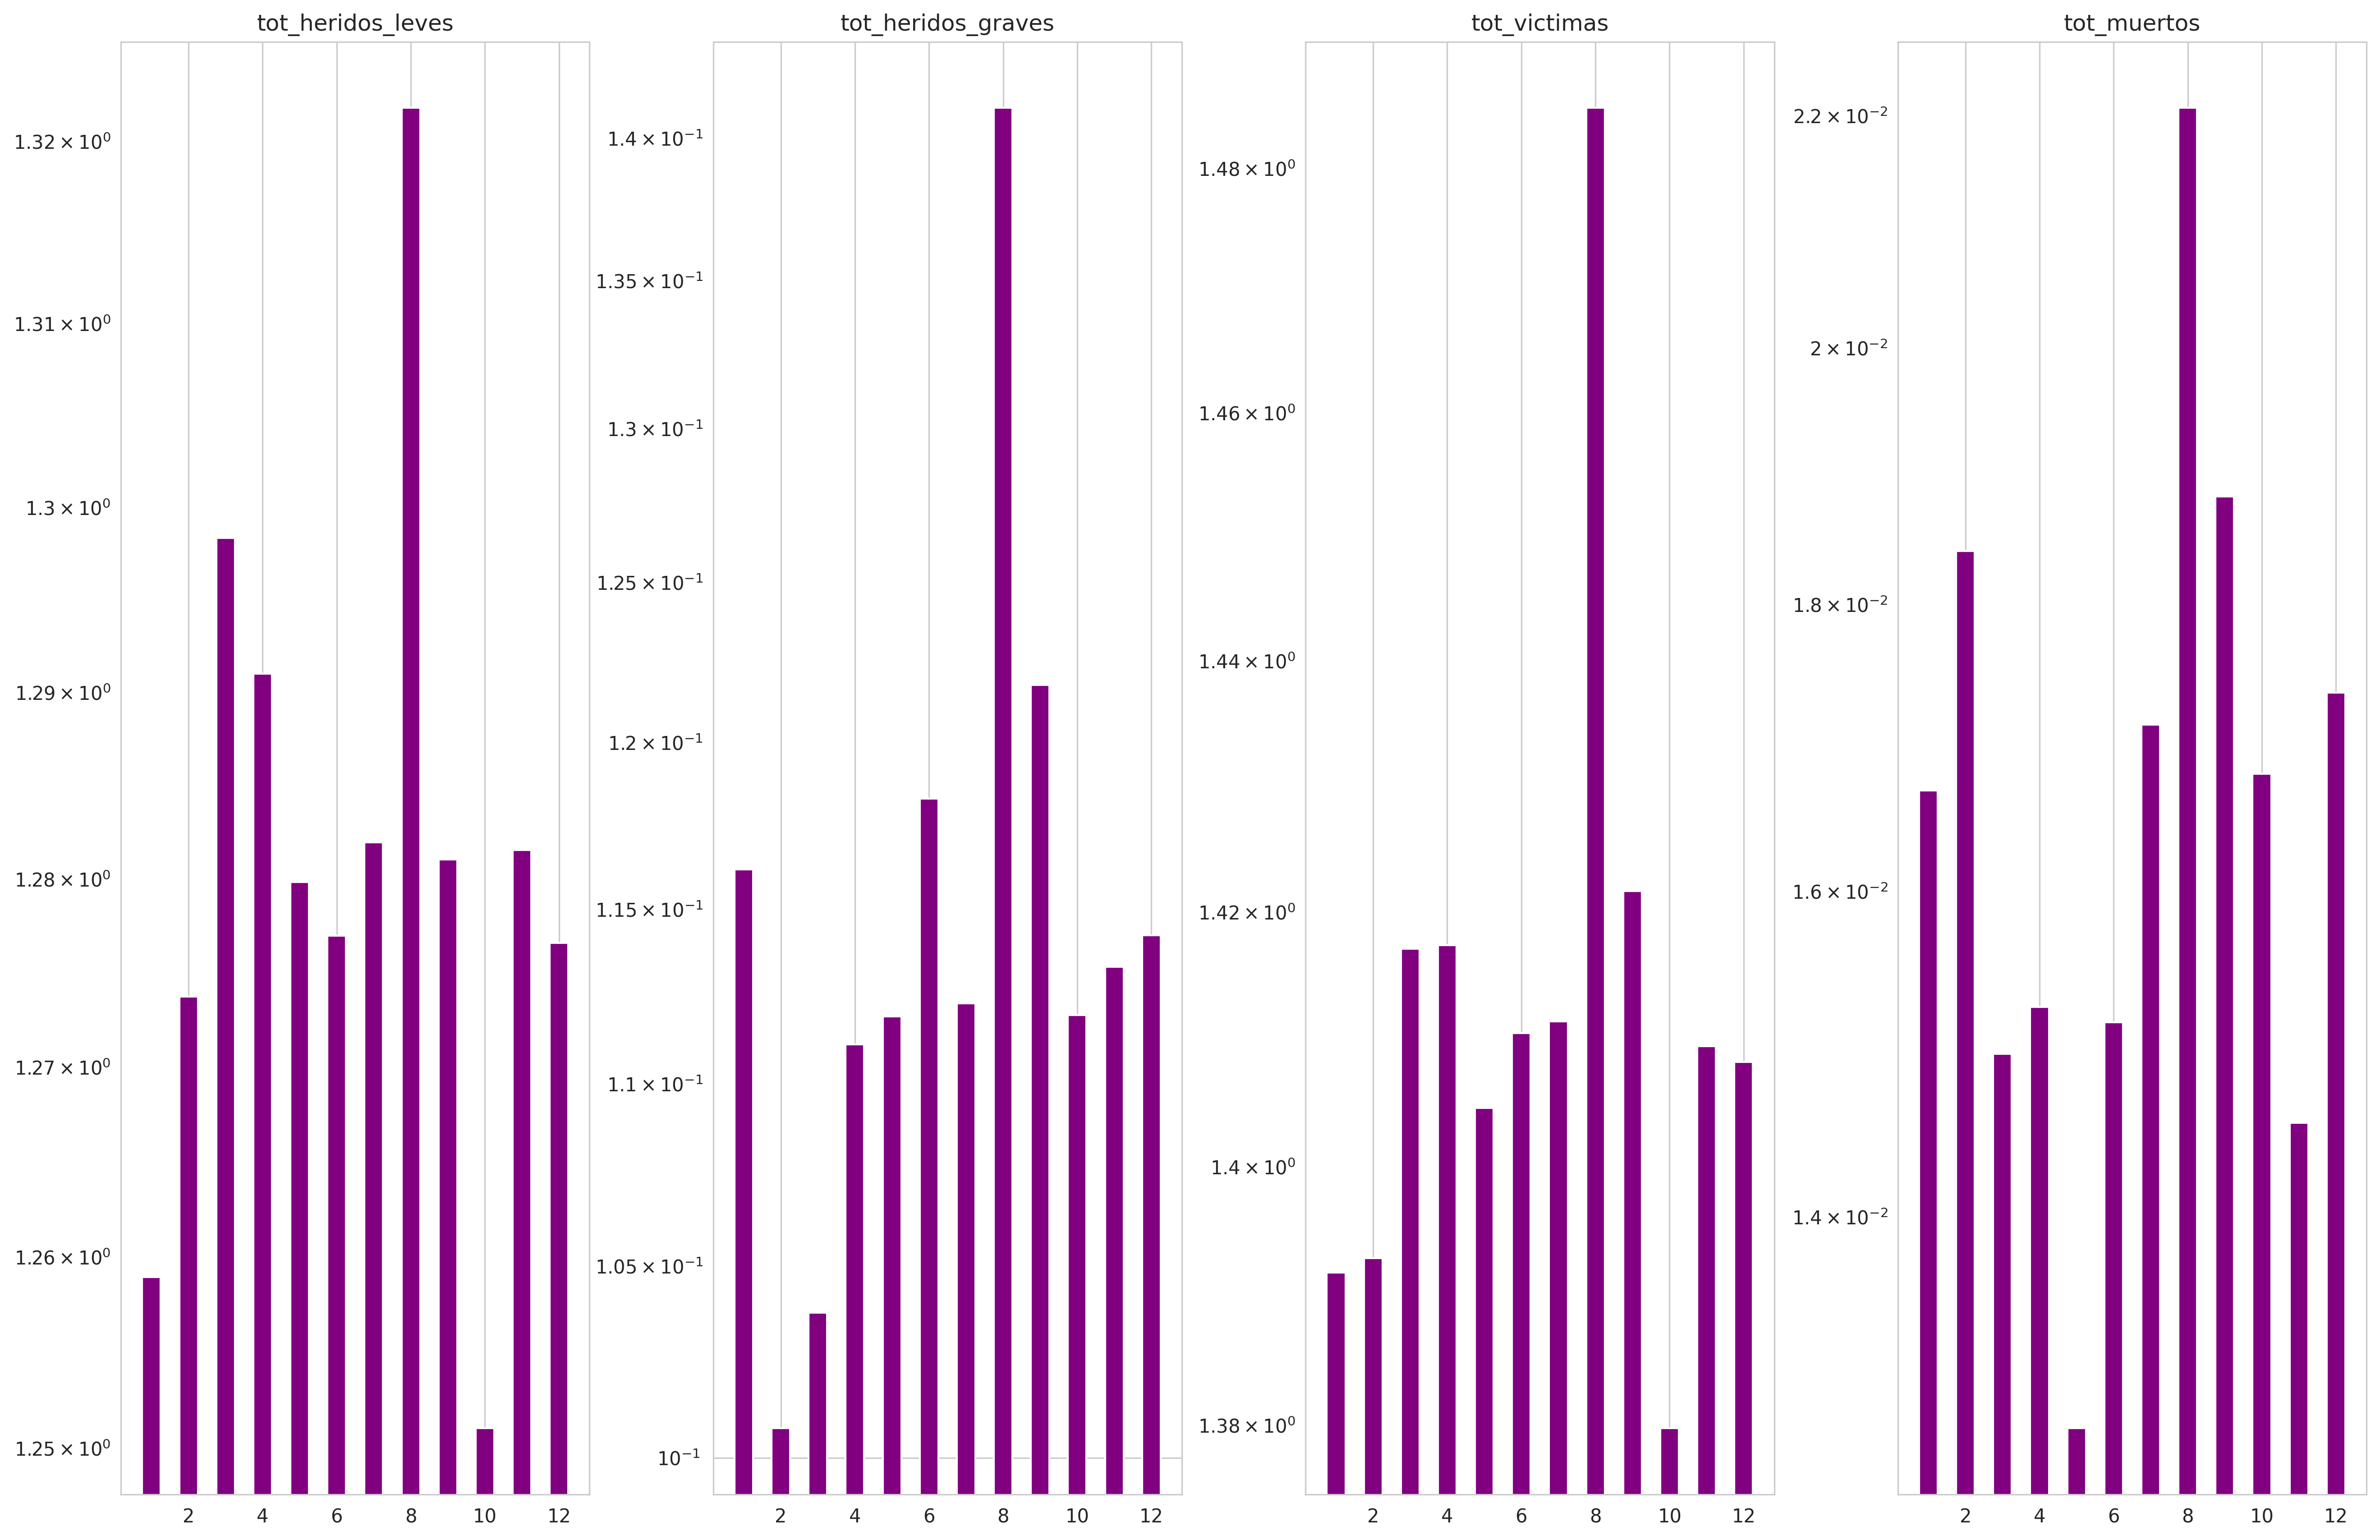
\includegraphics[width=1.1\linewidth]{img/influencia_mes}
	\caption{}
	\label{fig:influenciames}
\end{figure}

Es claro entonces que el mes de agosto es cuando los accidentes son más graves, el valor medio de cada uno de los atributos es el más elevado en este mes. Seguidamente se encuentra el mes de septiembre. Julio no es uno de los meses más afectados después de septiembre, pero también se encuentra en el periodo vacacional, por lo que lo vamos a incluir. 

Por lo tanto, siendo los meses de agosto y septiembre los más afectados por los accidentes de tráfico, nos vamos a centrar en el estudio de los accidentes en estos meses para intentar ver diferencias entre los tipos de accidentes que en esta época ocurren. Además, consideramos el mes de julio que, aunque también es un mes vacacional, presenta datos algo mejores, de modo que vamos a intentar analizar estas diferencias. 

Para seleccionar los datos de interés, en primer lugar nos quedamos con las instancias del dataset correspondientes a los meses considerados y a continuación tomamos los atributos numéricos relacionados con la gravedad del accidente que vamos a estudiar (total de víctimas, total de heridos leves y graves, total de muertos y total de vehículos implicados). Al \mintinline{python}{DataFrame} resultante de esta selección lo llamamos \mintinline{python}{caso1}.

\begin{minted}{python}
caso1=raw_data[((raw_data.mes == 7) | (raw_data.mes == 8) | (raw_data.mes == 9))]
cols=["tot_heridos_leves","tot_heridos_graves","tot_victimas",
		"tot_muertos","tot_vehiculos_implicados"]
caso1=caso1[cols]
\end{minted}
 Una vez tenemos nuestros datos separados del resto, convertimos el \mintinline{python}{DataFrame} a una matriz y normalizamos los datos, para que los algoritmos de clustering que vamos a usar calculen correctamente las distancias (eucídea en nuestro estudio) entre las instancias, obteniendo así la matriz \mintinline{python}{data_caso1}
\begin{minted}{python}
data_caso1 = to_matrix(caso1, cols)
data_caso1 = norm(data_caso1)
\end{minted}

\subsection{Análisis de los algoritmos}

Con el objetivo de agrupar los datos de nuestro primer caso de estudio en varios clusters, hemos usado los algoritmos de Kmeans y Agglomerative Clustering, ambos implementados en \mintinline{python}{sklearn.cluster}. 
\subsubsection{Algoritmo K-means}
Se trata de un algoritmo iterativo bastante eficiente en el que las instancias se van moviendo entre clusters hasta que se alcanza el conjunto de clusters deseado. Este algoritmo requiere que se prefije el número final de clusters \textbf{k} en que se agruparán las instancias, número que no tenemos por qué conocer a priori, por lo que hay que intentar determinar el valor más adecuado en cada caso. Además, asume que los clusters tienen forma convexa, de modo que los resultados empeoran si las formas fueran irregulares, y no trata bien con los datos ruidosos y los outliers. 

Sin embargo, vamos a iniciar nuestro estudio aplicando este algoritmo y analizando los clusters obtenidos con él. Para ello, debemos intentar buscar en primer lugar el número de clusters óptimo. Empezamos iterando en un rango de número de clusters de 2 a 20. Para cada número de clusters en este rango aplicamos el algoritmo y almacenamos en un vector las valores que nos dan el coeficiente de \underline{Silhouette} y el índice de \underline{Calinski-Harabaz} para el resultado obtenido en cada caso. Finalmente visualizamos las medidas obtenidas para este rango de número de clusters. Todo este proceso lo implementamos en una función llamada \mintinline{python}{calcular_k_SC}:
\begin{minted}{python}
 def calcular_k_SC(data,k_max):
	costs=[[] for i in range(2)] 
	for i in range(2,k_max):
	resultado = KMeans(n_clusters= i, random_state=150).fit(data)
	
	silhouette, calinski = measures_silhoutte_calinski(data, resultado.labels_)
	
	costs[0].append(silhouette)
	costs[1].append(calinski)
	
	fig, (ax1, ax2) =plt.subplots(1,2,figsize=(15,5))
	ax1.plot(range(2,k_max), costs[0])
	ax1.set_xlabel('Número de clusters')
	ax1.set_ylabel('Silhouette')
	
	ax2.plot(range(2,k_max), costs[1])
	ax2.set_xlabel('Número de clusters')
	ax2.set_ylabel('Calinski')
	plt.show()
	
calcular_k_SC(data_caso1,20)
\end{minted}
y el resultado obtenido para el rango de 2 a 20 con los datos de nuestro caso de estudio ha sido el siguiente:
\begin{figure}[h]
	\centering
	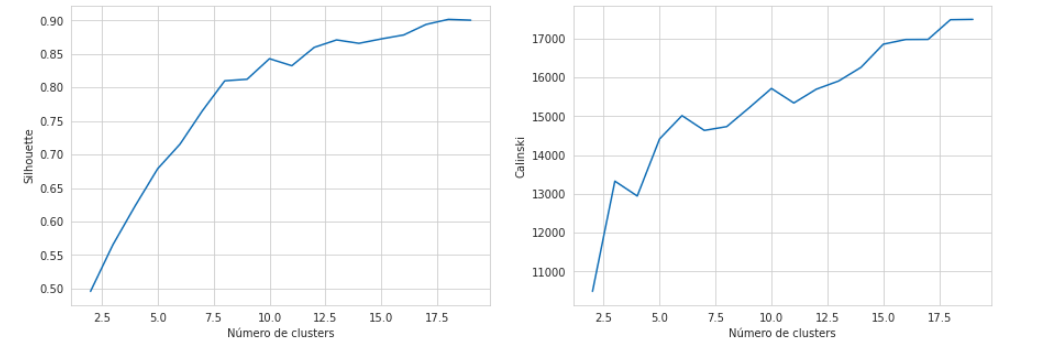
\includegraphics[width=1\linewidth]{img/calcular_sc1}
	\caption{}
	\label{fig:calcularsc1}
\end{figure}

de modo que los valores de estas métricas crecen con el número de clusters. Si aumentamos aún más el rango de estudio, estas medidas siguen creciendo indefinidamente con el número de clusters, de manera que no son un buen método para seleccionar el valor más apropiado (si cogemos un número muy elevado al final cada instancia o mínimo grupo de instancias formarán su propio cluster y no obtendremos información alguna, tendremos un alto nivel de sobreajuste. Este no es el objetivo del clustering).

Por lo tanto, decidimos optar por una técnica conocida como el '\textit{método del codo}' (ver \cite{4} y \cite{5} ). Para usar esta técnica calculamos  una métrica llamada \textbf{distortion}, que es la media de las distancias euclídeas al cuadrado entre los datos y el centro de su correspondiente cluster. Este valor se puede ver como la suma de las varianzas de cada cluster, de manera que cuanto menor sea, mejor es el agrupamiento.

Procedemos de la  misma manera que con las métricas anteriores de Silhouette y Calinski-Harabaz. Es decir, iteramos en un rango de número de clusters (para este caso lo hacemos entre 2 y 10), aplicamos el algoritmo para cada valor, guardamos el valor de distortion en cada caso en un vector y visualizamos los resultados:

\begin{minted}{python}
def calcular_k_elbow(data,k_max):
	distortions=[] 
	for i in range(2,k_max):
		kmeans = KMeans(n_clusters= i, random_state=200).fit(data)
		distortions.append(sum(np.min(cdist(data, kmeans.cluster_centers_, 
		'euclidean'),axis=1)) / data.shape[0])
		
	fig, ax =plt.subplots(figsize=(15,5))
	ax.plot(range(2,k_max), distortions)
	ax.set_title('The Elbow Method')
	ax.set_xlabel('Número de clusters')
	ax.set_ylabel('Distortions')
	plt.show()
calcular_k_elbow(data_caso1,10)
\end{minted}

\begin{figure}
	\centering
	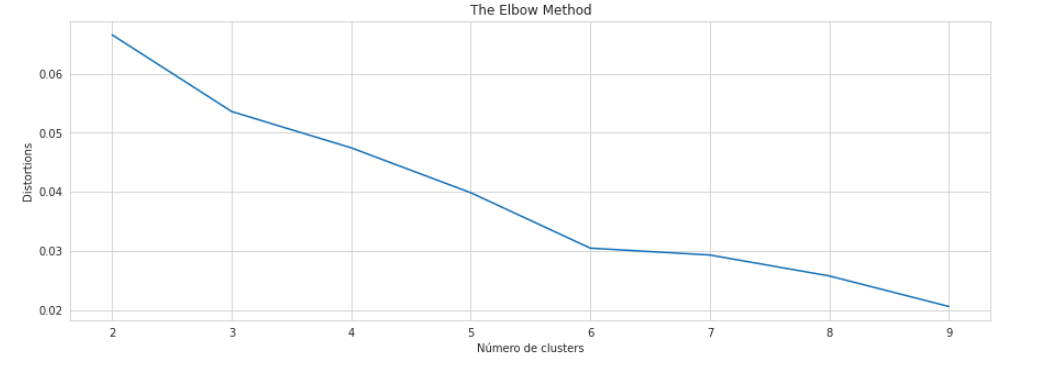
\includegraphics[width=1\linewidth]{img/elbow1}
	\caption{}
	\label{fig:elbow1}
\end{figure}

La mencionada técnica consiste en seleccionar el valor de k en el 'codo' de la gráfica. Es obvio que cuanto mayor sea el número de clusters el resultado mejora, pero a partir de un punto esta mejora es menor y lo que se produce es over-fitting. Los primeros clusters añaden mucha información pero una vez que se supera el número real de clusters existentes en los datos, la información aportada decrece enormemente, pues se están subdividiendo los clusters realmente existentes y se produce sobreajuste. En nuestro caso podemos observar que el punto crítico sería el 6:

Para aplicar el algoritmo hemos implementado la siguiente función, que además calcula las métricas de Silhouette y Calinski-Harabaz y muestra los resultado por pantalla:

\begin{minted}{python}
def k_means(data,k):
	kmeans = KMeans(n_clusters= k, random_state=200).fit(data)
	
	silhouette, calinski = measures_silhoutte_calinski(data, kmeans.labels_)
	
	print("Silhouette: {:3f}".format(silhouette))
	print("Calinsky: {:3f}".format(calinski))
	
	return kmeans
\end{minted}
Aplicándolo a nuestros datos con un número de clusters igual a 6 obtenemos los siguientes resultados:
\begin{minted}{python}
Silhouette: 0.735084
Calinsky: 15017.276290
\end{minted}

En la ejecución de \mintinline{python}{KMeans} hemos considerado todos los parámetros por defecto (excepto el número de clusters y \mintinline{python}{random_state}). Por ejemplo, la elección de los centros de los clusters iniciales la lleva a cabo automáticamente scikit-learn usando el esquema de inicialización \mintinline{python}{k-means++}. En cuanto a los pesos, hemos considerado a todos los atributos con igual relevancia en el agrupamiento.\\[0.1cm]

\textbf{Análisis de los clusters obtenidos}\\[0.05cm]

Pasamos ahora a analizar los clusters obtenidos con este algoritmo. Para ello vamos a realizar algunas visualizaciones. 

Empezamos viendo el tamaño de cada uno de los clusters creados: 
\vspace{3cm}

\begin{figure}[h]
	\centering
	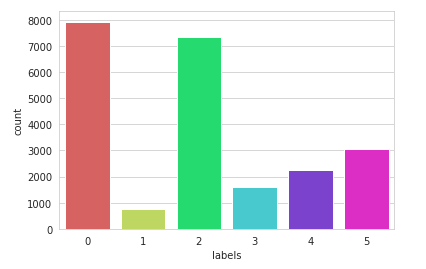
\includegraphics[width=0.5\linewidth]{img/count1}
	\caption{}
	\label{fig:count1}
\end{figure} 

por lo que los clusters con etiquetas 0 y 2 son los que recogen el mayor número de datos, seguidos por los clusters 5 y 4, siendo la diferencia entre los primeros y los segundos de unas $ 5000 $ instancias. El cluster 1 es el de menor tamaño, estando formado por menos de $ 1000 $ datos. 

Ahora visualizamos una imagen \mintinline{python}{pairplot} de nuestros datos etiquetados con el cluster que les ha sido asignado:
\begin{figure}[H]
	\centering
	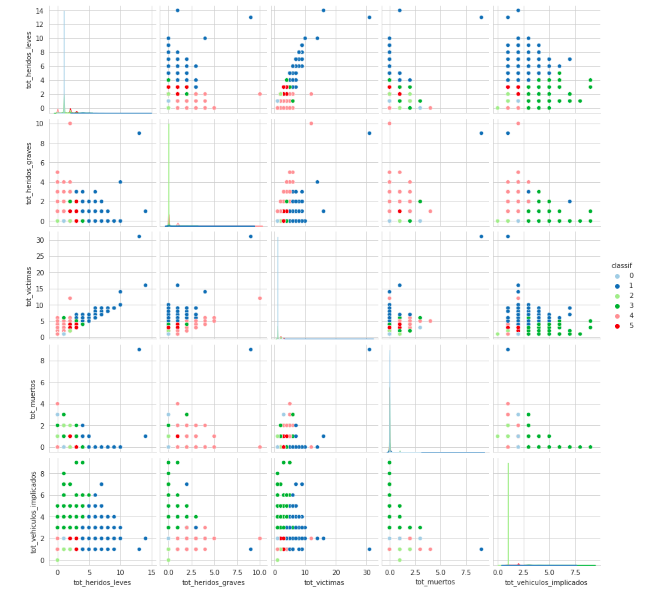
\includegraphics[width=1\linewidth]{img/pairplot1}
	\caption{}
	\label{fig:pairplot1}
\end{figure}
y de aquí podemos deducir que las variables total de heridos leves y total de vehículos implicados separan bastante bien los clusters 1 y 3, entre ellos y con el resto de clusters. Pero para el resto de variables y clusters no podemos obtener mayor información a partir de esta imagen.

Una imagen que sí nos puede ser de gran utilidad es el \mintinline{python}{heatmap}, que nos da información sobre los centroides de cada cluster, la cual suponemos representativa del respectivo cluster:

\begin{figure}[h]
	\centering
	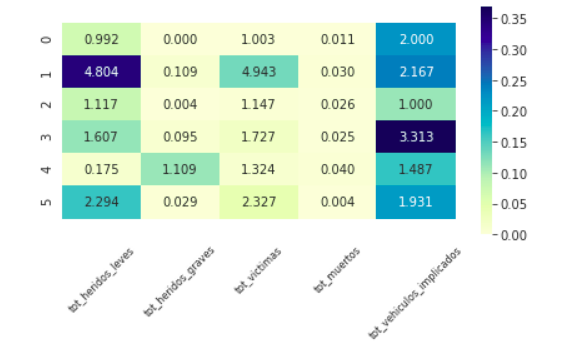
\includegraphics[width=1\linewidth]{img/heatmap1}
	\caption{}
	\label{fig:heatmap1}
\end{figure}

En este mapa cada cuadro muestra el valor que toma el centroide del cluster para la variable correspondiente y el color indica cómo de alto es este valor en relación a los demás valores que toma la variable. Antes de analizar los resultados que aquí aparecen, vamos a ver también los diagramas de cajas que muestran la distribución de las variables en cada cluster (los outliers han sido eliminados para una mejor visualización):
\vspace{8cm}
\begin{figure}[h]
	\centering
	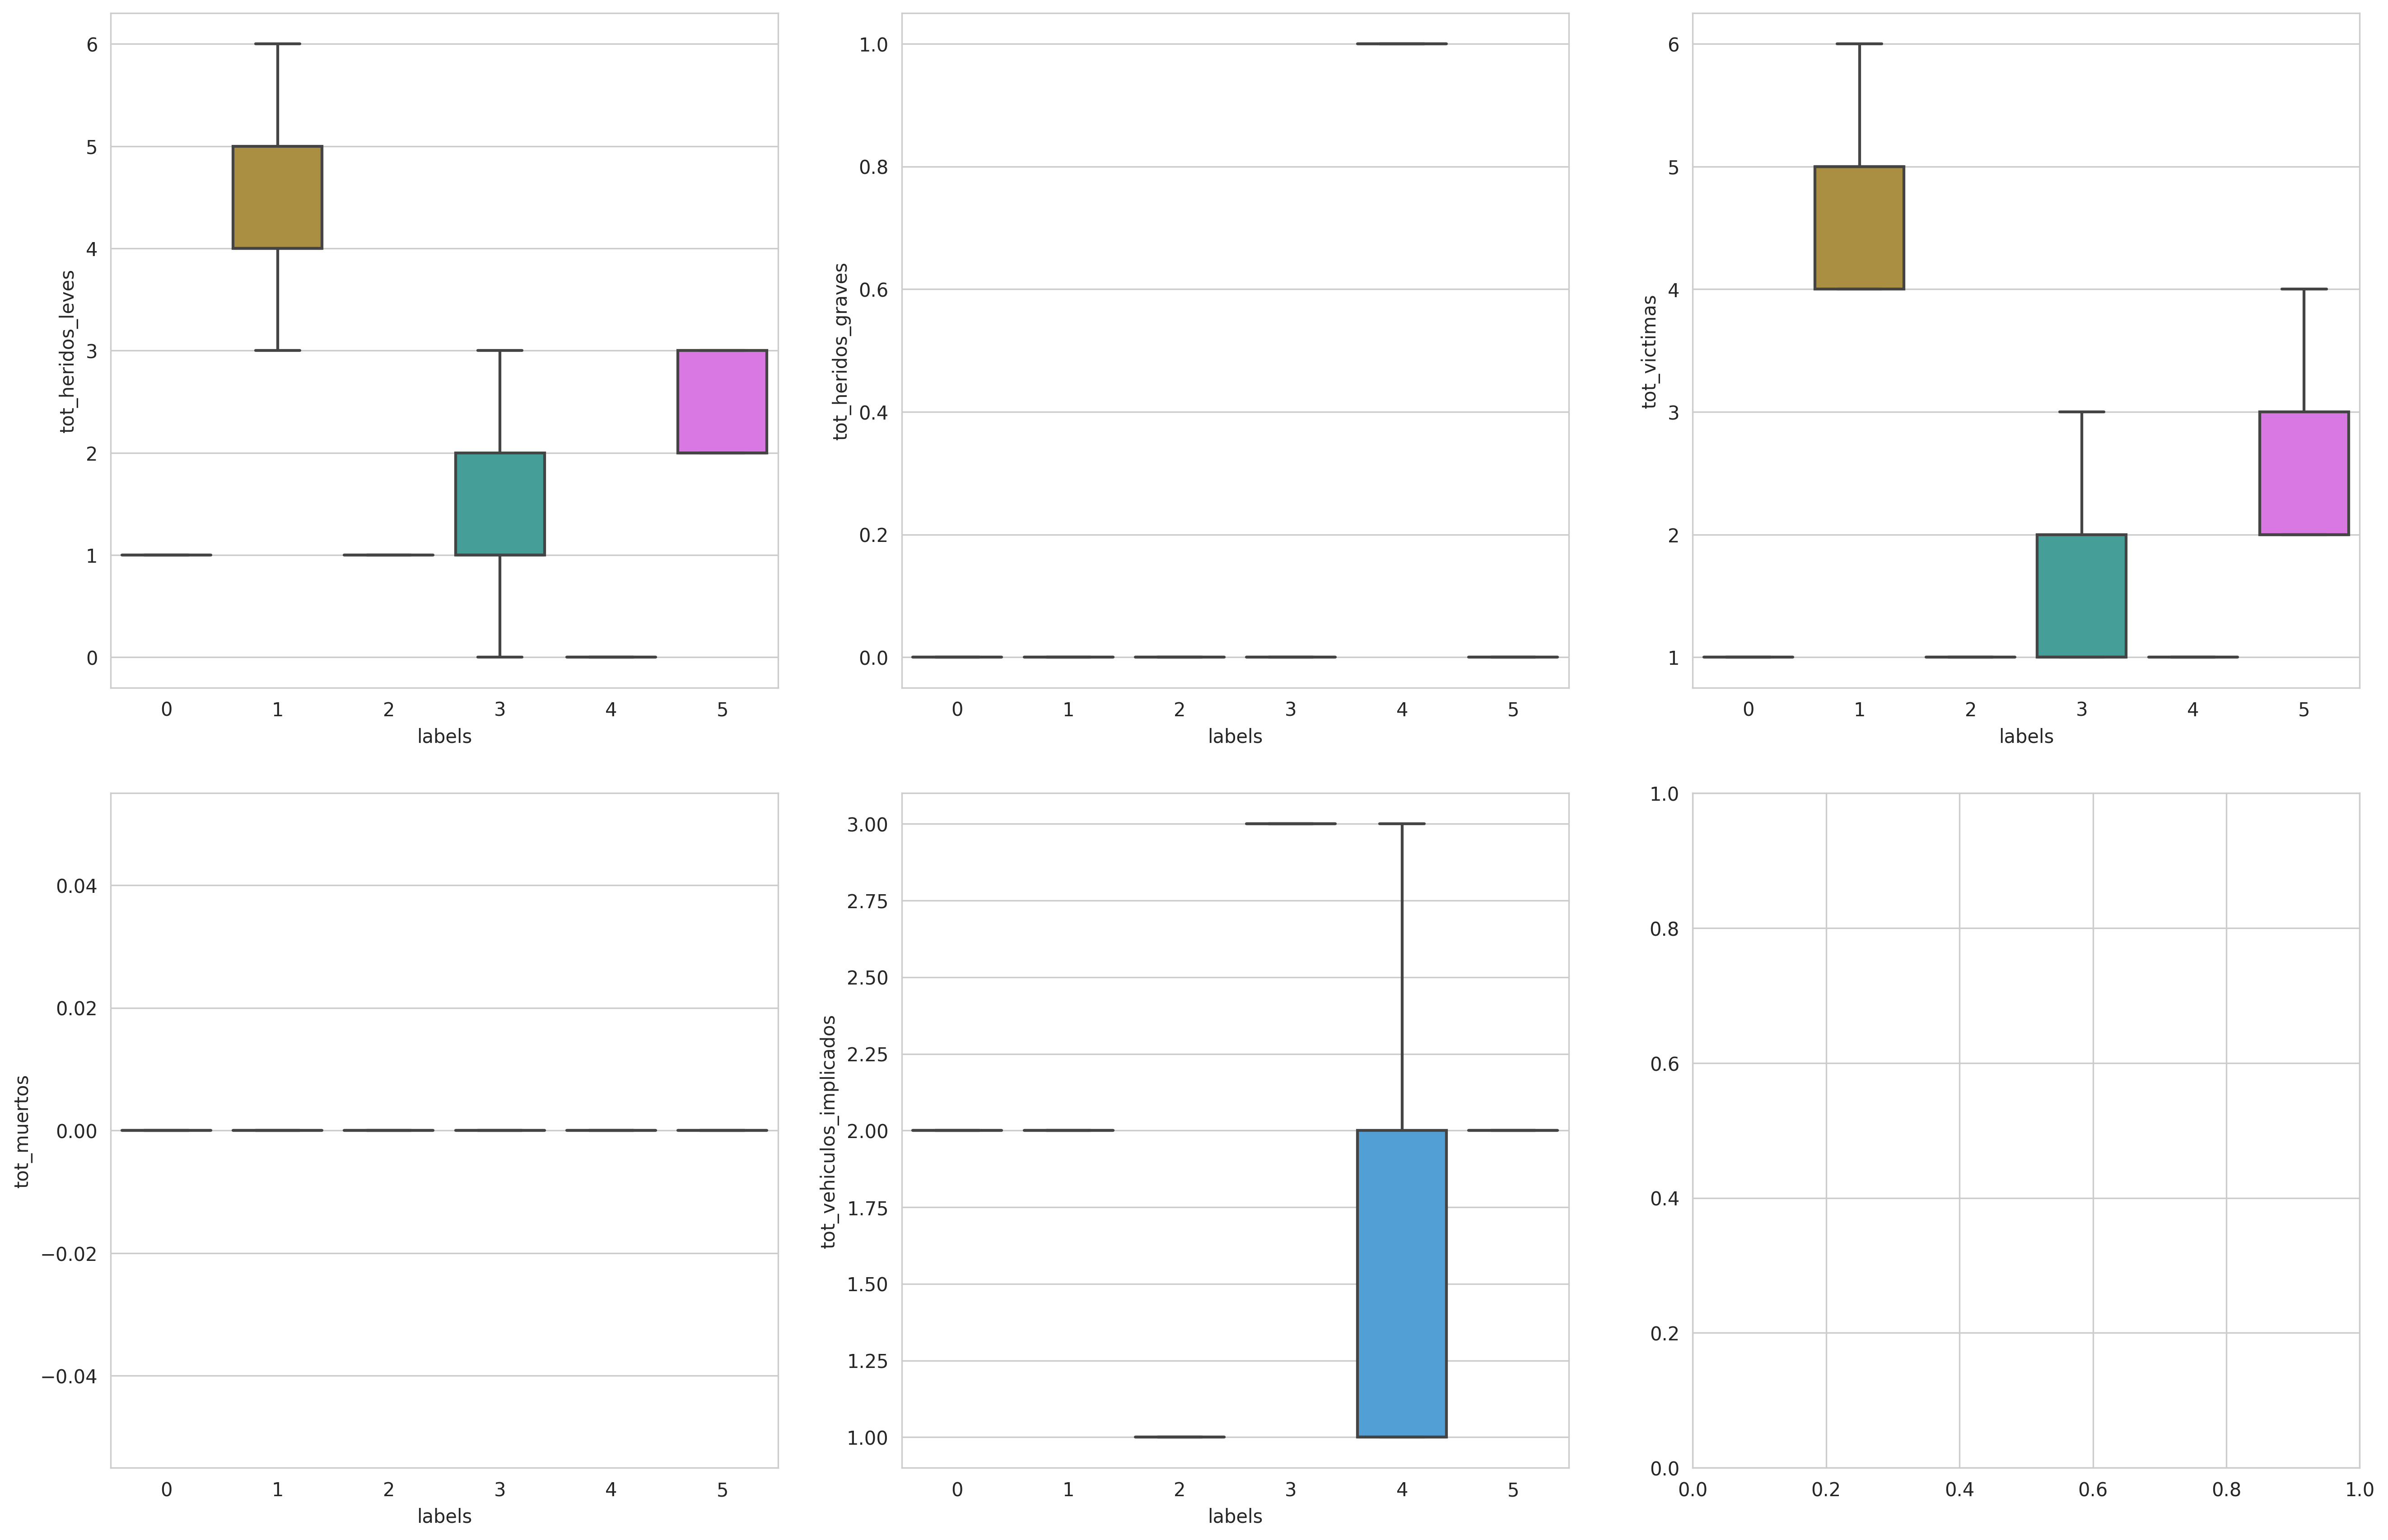
\includegraphics[width=1.1\linewidth]{img/cajas_cluster1}
	\caption{}
	\label{fig:cajascluster1}
\end{figure}

Ahora que disponemos de todas estas visualizaciones podemos ya analizar las características de cada uno de los clusters obtenidos con este algoritmo. 

\begin{itemize}
	\item El primer detalle que podemos observar, mirando el mapa de calor, es que el número de muertos toma una media de prácticamente cero en todos los clusters. Además, si observamos el diagrama de cajas, vemos que en todos los casos la distribución es degenerada en 0. Puesto que no hemos tenido en cuenta los outliers, el hecho de que la media de muertos no sea exactamente 0 es debido a estos valores atípicos, que hacen que esta aumente un poco. Así pues, podemos decir que, salvo en casos extremos y poco frecuentes, en el caso de estudio considerado el número de muertos por accidentes es prácticamente nulo. 
	\item Si nos fijamos en los diagramas de cajas de la variable \textit{total de heridos graves}, llegamos a practicamente la misma conclusión que con el número de muertos: casi todas las distribuciones son degeneradas en 0, y las medias son mayores que 0 en algunos casos por la influencia de los casos atípicos. Sin embargo, en este caso hay un cluster en el que la media del número de heridos graves es aproximadamente 1, y su distribución es degenerada en 1, de manera que en este cluster es donde se acumulan los datos que presentan mayor número de heridos graves. Pero aún así es un valor bastante bajo. Por tanto, podemos decir que esta variable es la que caracteriza al \underline{cluster 4} y que en nuesto caso de estudio el número de heridos graves es pequeño. 
	
	Para el resto de atributos de este cluster, observamos que el número de heridos leves es nulo en la mayoría de los casos (salvo casos atípicos) y el número total de víctimas tiene una distribución degenerada en 1 (es decir, todos los datos salvo excepciones tienen una única víctima, que se correspondería con la víctima herida grave que ya hemos comentado). Además, este cluster es el único que presenta una mayor dispersión en cuanto al número de vehículos implicados, variando desde 1 hasta 3 y siendo entre 1 y 2 en el 75\% de los casos (la media es 1.5).
	
	En definitiva, podemos decir que el cluster 4 está formado por los accidentes más graves dentro de los datos de que disponemos, donde el número de vehículos implicados es variable, pero siendo este sobre 1.5 en media.

	\item El \underline{cluster 0} está caracterizado porque el número de heridos leves es casi siempre 1 (en los outliers menos pues la media es algo inferior a 1), que coincide con el número total de víctimas, y el número de vehículos implicados en los accidentes es 2 (distribución degenerada en 2 y su media es 2, por lo que aquí podemos afirmar casi con total seguridad que en todos los accidentes de este cluster intervienen 2 vehículos).
	\item El \underline{cluster 2} no presenta ninguna característica destacable. Es bastante similar al cluster 0, salvo por el número de vehículos implicados, pues hay un único vehículo afectado en todos los accidentes de este cluster (media 1 y distribución degenerada en 1), a diferencia del anterior, en el que este valor era 2. Fijándonos en la media del número de heridos leves podríamos decir que en este cluster hay un número ligeramente superior de heridos, pero la diferencia es mínima. 
	
	\item Por su parte, el \underline{cluster número 1} es el que tiene el número de heridos leves más alto de todos los clusters de que disponemos (siendo la media de 4.8 heridos). La variabilidad en cuanto a los valores de este atributo es alta, pues se mueven entre 3 y 6 victimas estando la mitad de los datos entre 4 y 5 víctimas. En consecuencia, el número total de víctimas en este cluster es también el más alto y su distribución coincide casi totalmente con la del número de heridos leves (las diferencias se deben a los datos atípicos, por ejemplo algunos heridos graves o muertos que también se incluyen en el número total de víctimas). En cuanto a los vehículos implicados, queda claro que son 2 en casi todas las instancias, compartiendo esta característica con el cluster 0, aunque aquí la media es algo superior a 2, por lo que puede haber algunos casos en los que el número de vehículos sea mayor.
	
	\item Prestando atención al mapa de calor nos damos cuenta de que el \underline{cluster 3} es el que presenta un mayor número de vehículos implicados, con una media de 3.3. Su correspondiente diagrama de cajas muestra una distribución degenerada en 3, de donde podemos inferir que en prácticamente todos los accidentes de este cluster intervienen 3 vehículos, salvo en algunos casos en los que el número de implicados puede ser mayor (por lo que nos dice la media). En cuanto al número de heridos leves, vemos en los diagramas de cajas que el 50\% de la distribución presenta entre 1 y 2 heridos leves, teniendo como máximo 3 y como mínimo 0. Así, el valor de esta variable en este grupo presenta mayor variabilidad que en otros casos, como los clusters 0 y 2, y en media es algo superior. La distribución del número total de víctimas se corresponde casi totalmente con la del número de heridos leves, pues los heridos graves y los muertos tienen poca influencia en este caso. 
	
	\item Por último, en el \underline{cluster 5}, el número total de heridos leves tiene valores intermedios entre los que presenta el cluster 0 y el cluster 3, estando casi todos los datos situados entre 2 y 3 heridos. Como viene ocurriendo, la distribución del número total de víctimas es bastante similar a la del número de heridos leves, por los motivos ya explicados. Por su parte, los vehículos implicados, son 2 en prácticamente todos los casos, como ocurría en los clusters 0 y 1, pero es posible que en algunas situaciones este número sea un poco menor que en los grupos anteriores, ya que la media es 1.9.
	
\end{itemize}

\textbf{Conclusión:} En nuestro caso de estudio casi todos los accidentes se encuentran en los clusters 0 y 2, los cuales presentan el menor número de heridos leves y solo se diferencian en los vehículos implicados, es decir, en casi todos los accidentes de nuestro estudio hay un único herido leve y uno o dos vehículos implicados. Estos van seguidos por el cluster 5, en el que el número de heridos leves es algo superior (en torno a 2 y 3) y los vehículos implicados vuelven a ser 2. El cluster 4 es el que registra accidentes de mayor gravedad, pero a él pertenecen menos instancias que en los casos anteriores. Además, los accidentes en los que el número de víctimas es mayor (leves), recogidos en el cluster 1, suponen la minoría de los datos. En cuanto a los vehículos implicados, son en su mayoría 1 o 2, pues el cluster 3, con las instancias con un mayor número de vehículos, incluye menos accidentes que los cluters 0, 2 y 5.  Por lo tanto, los accidentes estudiados son casi siempre leves, con uno o dos vehículos afectados. Como excepción tenemos grupos pequeños de datos en los que hay algún herido grave, más heridos leves y una mayor cantidad de vehículos. 

\subsubsection{Agglomerative Clustering}

Este algoritmo forma parte de los métodos jerárquicos de clustering, los cuales tratan de formar clusters anidados mediante su sucesivo agrupamiento o división. En concreto, nuestro algoritmo lleva a cabo la primera de las opciones de la siguiente manera: cada instancia constituye al principio su propio cluster y en cada paso se van mezclando los clusters resultantes de la iteración anterior, teniendo en cuenta algún criterio que usa una medida de distancia. \mintinline{python}{sklearn} ofrece varias opciones para llevar a cabo esta mezcla, pero nosotros usaremos aquí la opción por defecto que se denomina \textit{Ward}. Este criterio busca fusionar el par de cluster que generen un agrupamiento tal que la media de la distancia cuadrática de cada elemento al centroide (lo que hemos llamado antes \textit{distortions}) sea mínima. Se tiene usa para ello la distancia euclídea. 

Los algoritmos jerárquicos conllevan un mayor coste computacional que el algoritmo de K-means, tanto por tiempo de ejecución como por requisitos de memoria, de manera que no son muy apropiados cuando se trata con grandes cantidades de datos. Sin embargo, esto no supone un gran problema en nuestro caso. Por otra parte, estos algoritmos hacen posible visualizar la jerarquía de los clusters y los pasos que tienen lugar para formar los grupos, mediante lo que se conoce como denograma, con lo que estos algoritmos son algo más interpretables. Nosotros no hemos llevado a cabo esta visualización, pues con las demás realizadas es suficiente para poder interpretar correctamente los clusters, aunque también se podría haber hecho. 

El número final de clusters en este algoritmo no siempre tiene por qué ser prefijado. Se puede seleccionar un límite para la distancia en el criterio de fusión, a partir del cual no se siguen mezclando los clusters en otros mayores, de manera que el número final de clusters queda determinado automáticamente por este límite. No obstante, nosotros hemos optado por la otra opción, es decir, fijamos un número de clusters y este límite no lo tenemos en cuenta, puesto que ya hemos visto el método del codo que funciona bastante bien y podemos usarlo también para el algoritmo aglomerativo.   

Con el fin de buscar el número óptimo de clusters, implementamos en este caso la función \mintinline{python}{calcular_k_hierarchical}. Su funcionamiento es idéntico al de \mintinline{python}{calcular_k_elbow}, que ya hemos comentado, con la excepción de que en esta nueva función se usa el algoritmo aglomerativo y los centroides de los clusters deben ser calculados explícitamente porque este algoritmo no los devuelve, como era el caso de Kmeans. 

\begin{minted}{python}
def calcular_k_hierarchical(data,k_max):
	distortions=[] 
	for i in range(2,k_max):
	resultado = AgglomerativeClustering(n_clusters= i).fit(data)
	
	#Calcular los centros
	centros=pd.DataFrame(data)
	centros['labels']=resultado.labels_
	centros=np.array(centros.groupby('labels').mean())
	distortions.append(sum(np.min(cdist(data, centros, 
	'euclidean'),axis=1)) / data.shape[0])
	
	fig, ax =plt.subplots(figsize=(15,5))
	ax.plot(range(2,k_max), distortions)
	ax.set_title('The Elbow Method')
	ax.set_xlabel('Número de clusters')
	ax.set_ylabel('Distortions')
	plt.show()
calcular_k_hierarchical(data_caso1,15)
\end{minted}

En la última línea hemos ejecutamos la función con los datos de nuestro caso de estudio y para un rango de valores de entre 2 y 15, obteniendo la siguiente representación: 

\begin{figure}[H]
	\centering
	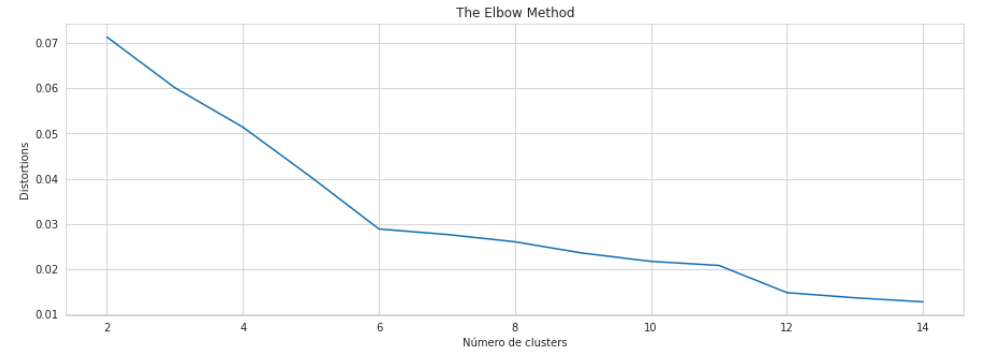
\includegraphics[width=0.9\linewidth]{img/elbow3}
	\caption{}
	\label{fig:elbow3}
\end{figure}


donde claramente se distingue que el valor óptimo del número de clusters debería ser 6. 

Para ejecutar el algoritmo, consideramos la función \mintinline{python}{agglomerative(data,k)}, que llama a \mintinline{python}{AgglomerativeClustering} con el número de clusters y los datos proporcionados como argumento, nos devuelve el resultado de aplicar dicho algoritmo y muestra por pantalla los valores de los coeficientes de Silhouette y Calinski-Harabaz:

\begin{minted}{python}
def agglomerative(data,k):
	resultado = AgglomerativeClustering(n_clusters= k).fit(data)
	
	silhouette, calinski = measures_silhoutte_calinski(data, resultado.labels_)
	
	print("Silhouette: {:3f}".format(silhouette))
	print("Calinsky: {:3f}".format(calinski))
	
	
	return resultado
\end{minted}

y el resultado tras ejecutarla con nuestros datos y un número de clusters igual a 6 es el siguiente:
\begin{minted}{python}
Silhouette: 0.730737
Calinsky: 12399.641611
\end{minted}

\textbf{Análisis de los clusters obtenidos}\\[0.05cm]

Como hicimos con el algoritmo anterior, visualizamos mediante distintos tipos de gráficas los clusters obtenidos tras ejecutar el algoritmo aglomerativo. 

El primer gráfico a tener en cuenta es un \mintinline{python}{countplot}, para hacernos una idea de la cantidad de datos que se han agrupado en cada uno de los clusters formados:

\begin{figure}[h]
	\centering
	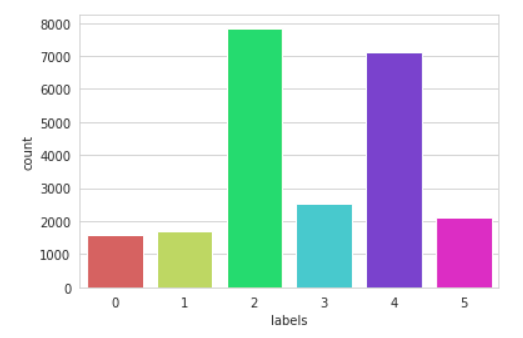
\includegraphics[width=0.7\linewidth]{img/count3}
	\caption{}
	\label{fig:count3}
\end{figure}

Observando esta gráfica nos damos cuenta de que el cluster que recoge la mayor parte de los datos es el número 2, con casi 8000 instancias, seguido de muy cerca por el cluster número 4 (la diferencia entre ambos es de menos de 1000 instancias). A continuación se encuentran los clusters 3 y 5, que contienen alrededor de 20000 datos, siendo los grupos 0 y 1 los que presentan el menor tamaño con unas 15000 instancias.

Veamos ahora el \mintinline{python}{pairplot} con los datos etiquetados por el número de cluster correspondiente:  
\vspace{15cm}

\begin{figure}[h]
	\centering
	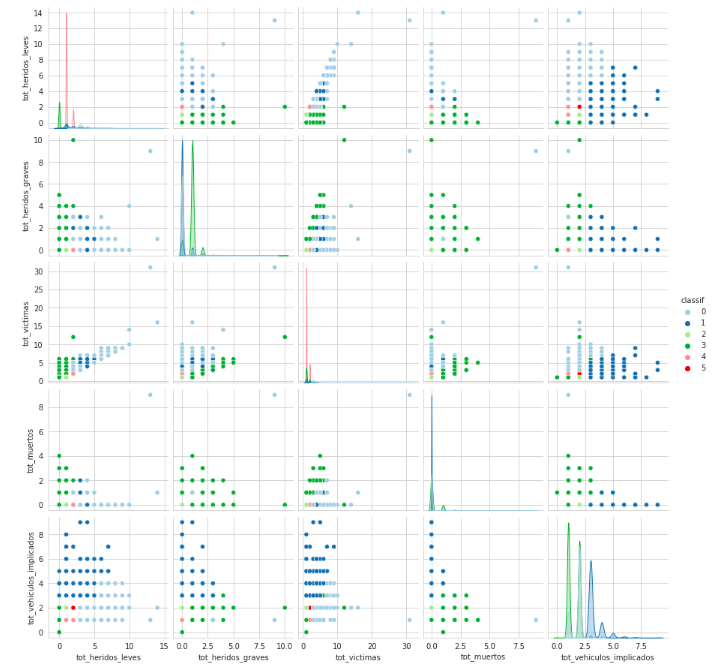
\includegraphics[width=1.1\linewidth]{img/pairplot3}
	\caption{}
	\label{fig:pairplot3}
\end{figure}

Gracias a esta imagen nos damos cuenta de que los atributos de total de heridos leves y total de vehículos implicados distinguen bastante bien los clusters número 0 y 1. Por otra parte, el atributo de total de vehículos, junto con el total de heridos graves o el total de muertos, permite distinguir el cluster 1 y 3. A parte de esta información, no podemos deducir nada más significativo con esta representación. 

Mostramos en las siguientes figuras el mapa de calor de los centroides resultante (Figura 2.13) y los diagramas de cajas para cada uno de los atributos considerados sin tener en cuenta los outliers (Figura 2.14):
\vspace{3cm}
\begin{figure}
	\centering
	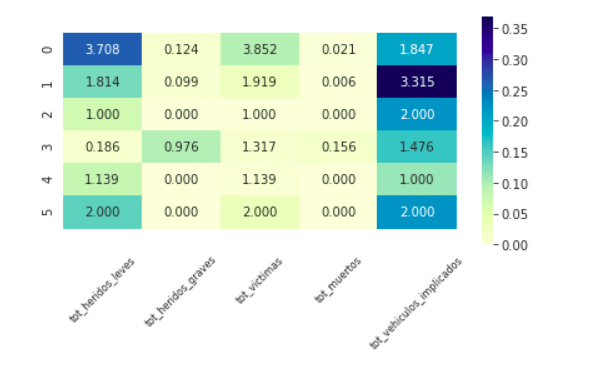
\includegraphics[width=0.9\linewidth]{img/heatmap3}
	\caption{}
	\label{fig:heatmap3}
\end{figure}
\begin{figure}[H]
	\centering
	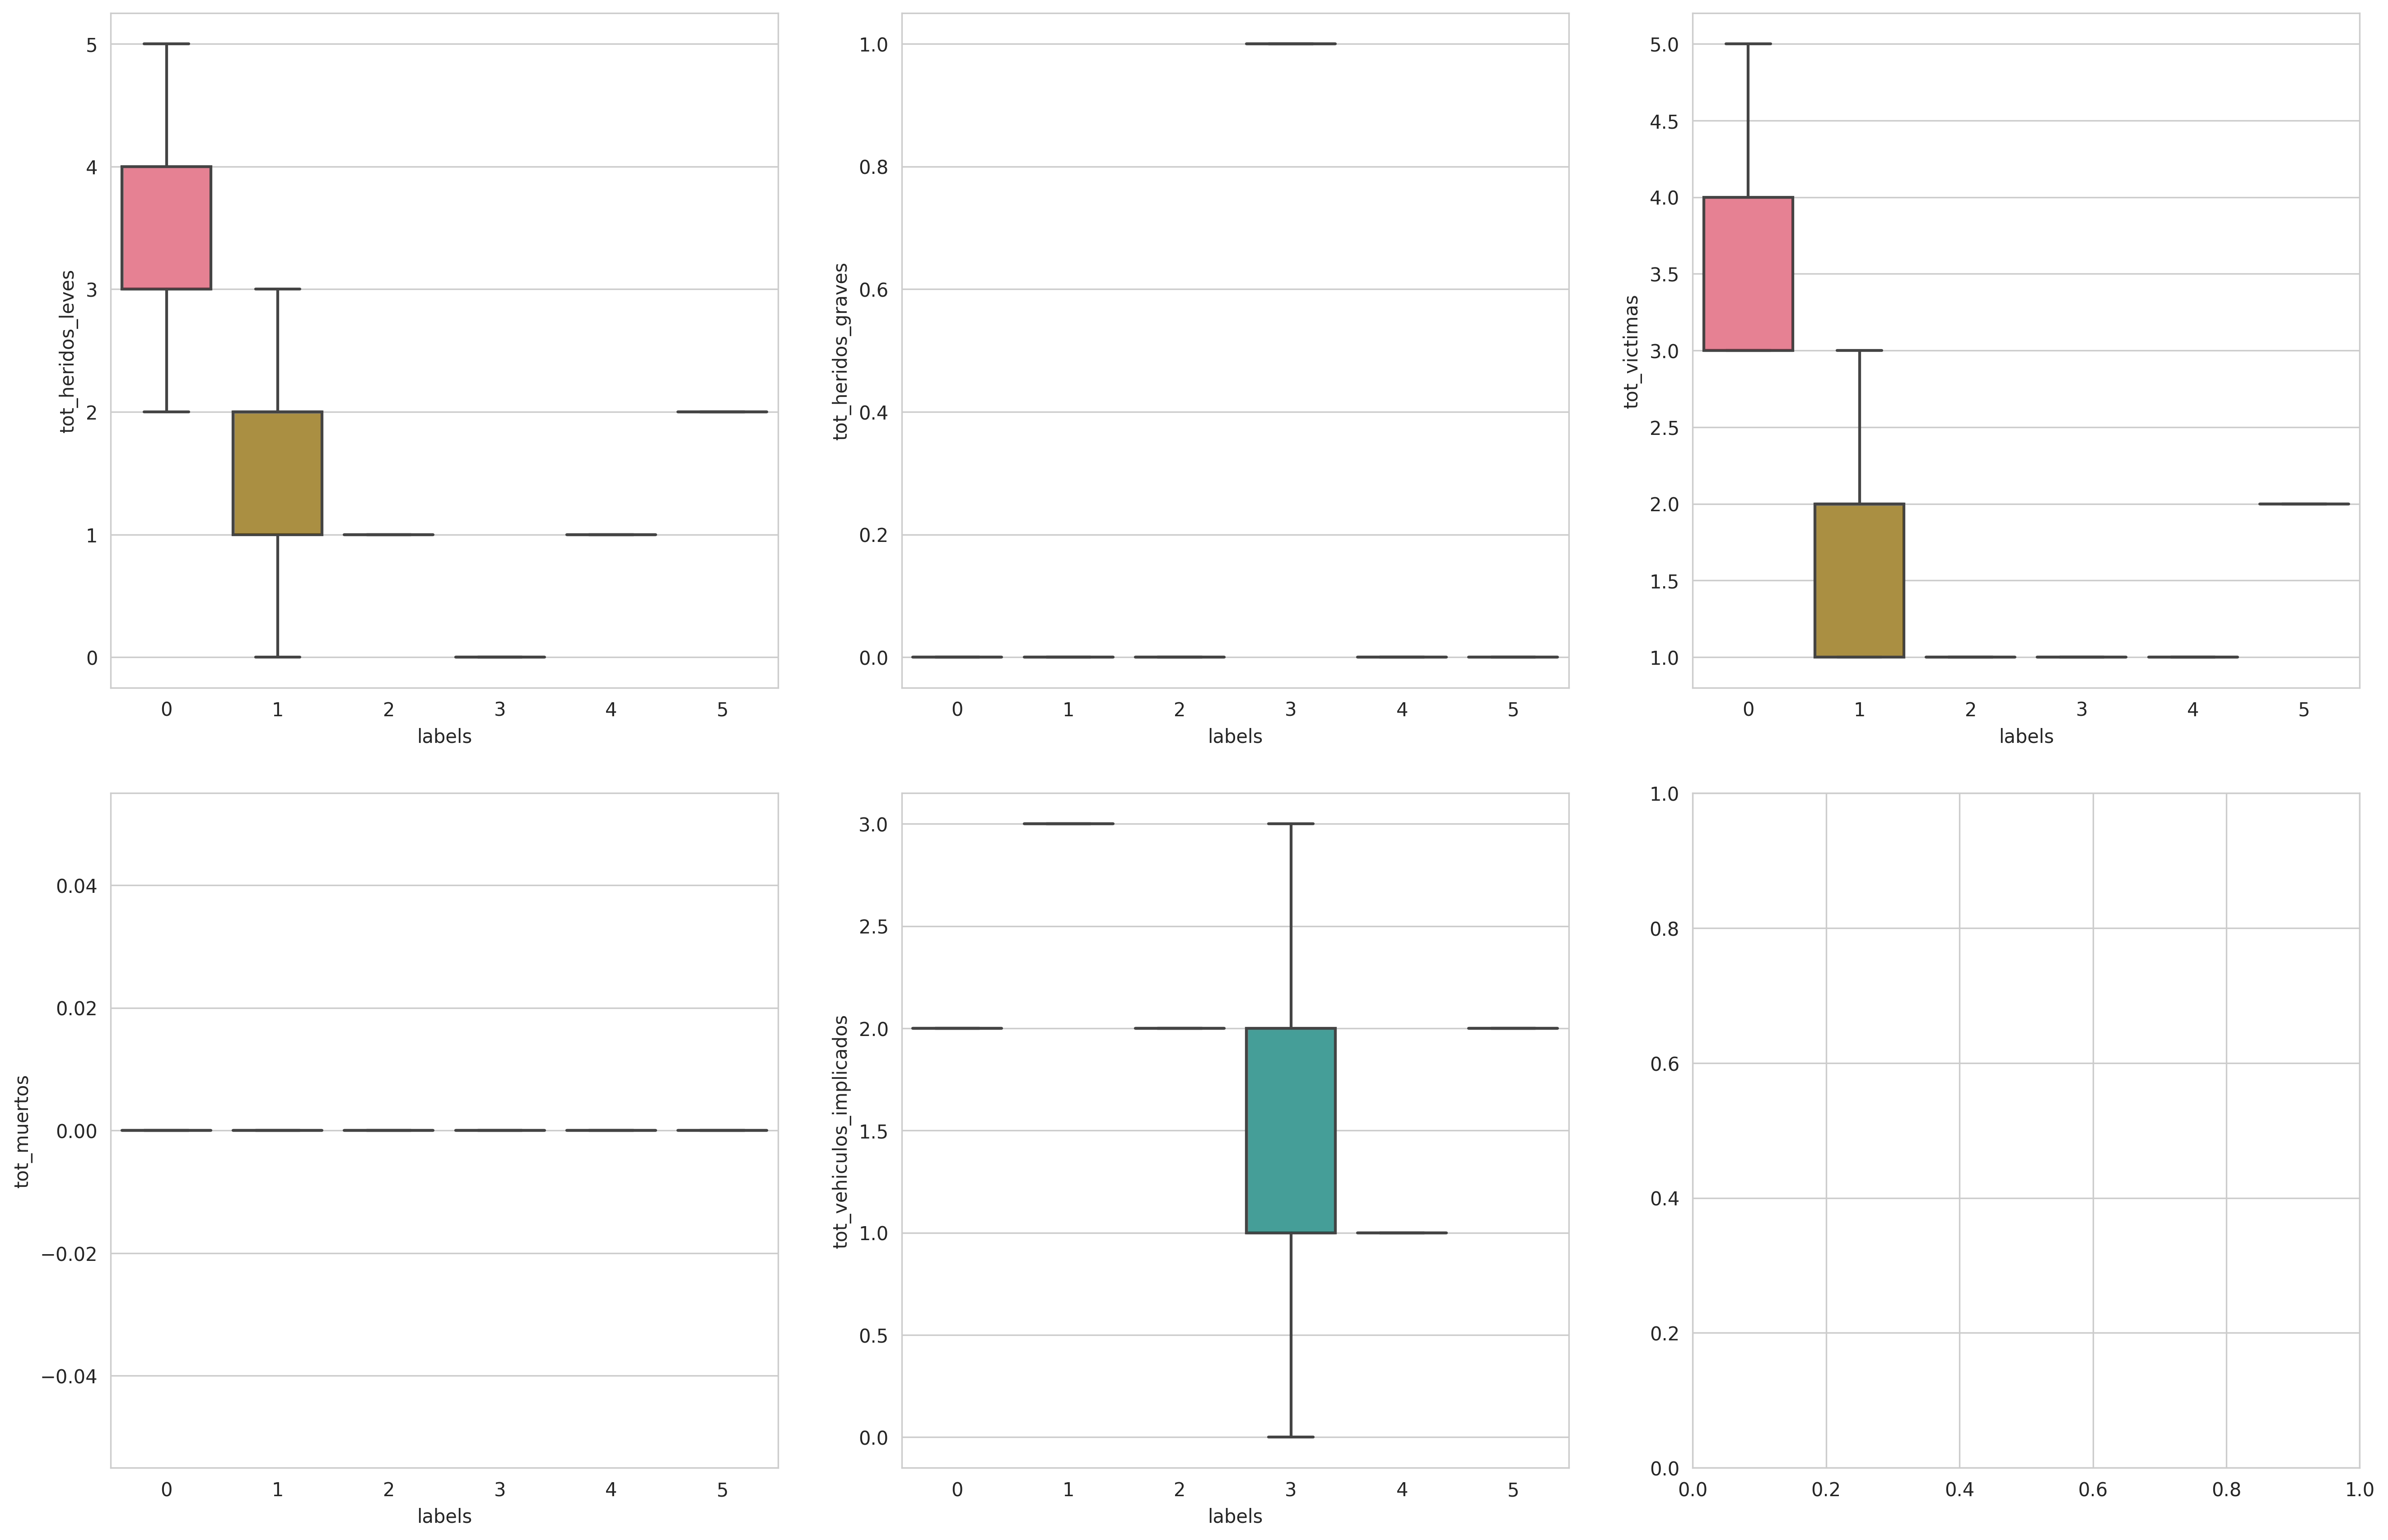
\includegraphics[width=1.1\linewidth]{img/cajas_cluster3}
	\caption{}
	\label{fig:cajascluster3}
\end{figure}

Estudiemos entonces las características de cada uno de los grupos obtenidos y la influencia de los atributos considerados en nuestro caso de estudio. 
\begin{itemize}
	\item Fijándonos en el mapa de calor y los diagramas de cajas correspondientes a la variable total de muertos, nos damos cuenta de que en todos los clusters esta variable toma el valor 0 para la mayoría de los datos, pues nos encontramos en todos los casos con una distribución degenerada en 0 de dicha variable. Además, la media del número total de muertos es prácticamente 0 siempre, salvo en algunos clusters para los que esta es algo superior a 0, pero podemos suponer que este ligero incremento es debido a datos atípicos que no son considerados. Por lo tanto, deducimos que el número de muertos no es un atributo importante que aporte información para nuestro caso de estudio o que nos permita distinguir entre diferentes grupos de datos. 
	
	\item  Por otro lado, si prestamos atención al número total de heridos graves, podemos percatarnos de que el único cluster que presenta algunos heridos graves es el \underline{cluster número 3}, en el cual la gran mayoría de los accidentes tienen un herido grave, puesto que la distribución de dicha variable es degenerada en 1 y su media es aproximadamente 1 (para algunos datos excepcionales, no considerados en la representación del diagrama de cajas, el número de heridos graves puede ser nulo, ya que la media es algo inferior a 1). En los demás grupos este atributo toma el valor 0 en casi todos los datos que estos contienen, pues, como ocurría con el número total de muertos, su correspondiente distribución es degenerada en 0 y la media es casi 0. Por lo tanto, salvo casos atípicos, el cluster 3 es el que contiene los datos con algún herido grave.  
	
	Con respecto a los valores de los demás atributos en el cluster 3, podemos destacar que el número de heridos leves es 0 en prácticamente todos los accidentes (para una minoría puede no ser nulo, de ahí que la media sea ligeramente superior a 0), con lo que el número total de víctimas coincide por lo general con el número de heridos graves, siendo su media, por lo tanto, aproximadamente 1 y su distribución degenerada en 1. 
	
	Otro aspecto a destacar de este cluster es que la variable 'número de vehículos implicados' presenta la distribución con mayor dispersión de entre todos los clusters, variando el valor entre 0 y 3 y estando la mitad de los datos concentrados en torno a 1 y 2. Es curioso que haya accidentes con un total de 0 vehículos implicados, lo cual puede ser debido a algún error en los datos o a accidentes relacionados con peatones. El alto grado de dispersión de este atibuto en este grupo puede deberse al hecho de que aquí se recogen los accidentes con algún herido grave, y dichos accidentes pueden ser de cualquier tipo, de manera que es posible que intervenga cualquier número de vehículos.
	
	\item Dejando a un lado el análisis de los atributos y centrándonos en los grupos más destacables obtenidos, salta a la vista que el \underline{cluster 0} es el que contiene los datos con el mayor número de heridos leves. Este número varía entre 2 y 5 heridos, con el 50\% de los accidentes presentando entre 3 y 4 heridos y estando la media situada en 3,7. Como el número de heridos graves y el total de muertos es 0 en casi todos los datos de este cluster (al igual que ocurre en los demás grupos), excepto en algunos accidentes atípicos en los que dichas cantidades pueden superar el 0, la media y distribución del número total de víctimas coincide casi totalmente con la del número de heridos leves. Por otro lado, los vehículos implicados en este cluster son casi siempre 2, aunque para algunos datos puede ser un único vehículo el afectado, puesto que la media es algo inferior a 2. Es raro que para ser el cluster con el mayor número de heridos leves, el número de vehículos afectados sea bajo. Una explicación probable es que en los vehículos afectados viajaran más de una persona o también que se vieran afectados peatones. 
	
	\item Otro grupo destacable es el \underline{número 1}, claramente distinguible por ser el que contiene los datos con el número más alto de vehículos implicados, siendo este 3 en la mayoría de los casos (distribución degenerada en 3), pudiendo presentearse accidentes con un número mayor, ya que la media es ligeramente superior a 3. El número total de heridos leves en este caso tiene una distribución bastante dispersa, pues dicho número varía entre 0 y 3, con la mitad de los datos entre 1 y 2 y siendo la media de 1,8. Como ocurría en el caso anterior, la distribución del número total de víctimas es casi idéntica a la del número de heridos leves, por los mismos motivos ya explicados. En estos accidentes, caracterizados porque el número de vehículos es casi siempre 3, puede haber casi cualquier número de víctimas, dependiendo de la gravedad del accidente. Por eso este atributo presenta una dispersión mayor que en otros grupos. 
	
	\item Pasamos ahora a analizar el \underline{cluster número 5} en el que curiosamente observamos que el número total de heridos leves es exactamente 2 en todos los datos que contiene, al igual que el número total de vehículos implicados. Además, el número de heridos graves y de fallecidos es exactamente 0 en todos los casos, con lo que el número de víctimas coincide con el de heridos leves completamente, es decir, es siempre 2.
	
	\item En todos los accidentes del \underline{cluster número 2} intervienen también 2 vehículos. La única diferencia con el grupo anterior está en los heridos leves, pues en este caso dicho atributo toma un valor de 1 para todos los datos, que coincide con el número total de víctimas. 
	
	\item Por último, el \underline{cluster 4}, queda caracterizado porque los vehículos implicados son 1 en todas las instancias que recoge. 
	En cuanto al total de heridos leves, dicha variable presenta una distribución degenerada en 1, pero su media es algo superior a este valor, por lo que podemos deducir que casi siempre resulta un herido leve en estos accidentes, salvo en los datos que son considerados outliers, en los que dicho número total puede ser superior. Como de nuevo el total de heridos graves y muertos es completamente nulo, el total de víctimas es igual al número de heridos leves. 
\end{itemize}

\textbf{Conclusión:} Nos encontramos ante un conjunto de datos donde la mayoría de ellos presentan un único herido leve, consecuencia de un accidente en el que intervienen 1 (cluster 4) o 2 vehículos (cluster 2). Otra parte de los datos, menor que la anterior, recoge accidentes en los que resultan 2 heridos leves y se ven implicados 2 vehículos (cluster 5). También es probable que alguien salga herido gravemente en los accidentes que aquí consideramos, pues el cluster 3, que contiene los datos con esta característica, tiene un tamaña considerable. En dichos accidentes, el número de vehículos implicados es variable (entre 0 y 3), siendo normalmente 1 o 2.  

En menor medida, pero de manera probable, nos encontramos con accidentes en los que el número de vehículos implicados es mayor (cluster 1), a saber, 3, y el número de heridos leves varía entre 0 y 3, siendo por lo general 1 o 2. Además, aparecen datos con un número de heridos leves más elevado (cluster 0), en concreto, con 3 o 4 heridos leves, pudiendo alcanzar incluso los 5 heridos, donde los vehículos que intervienen son casi siempre 2. 

\newpage
\subsubsection{Comparación de ambos algoritmos}
Vamos ahora a comparar los resultados proporcionados por cada uno de los dos algoritmos estudiados. Podemos comprobar que el número final de clusters para ambos es el mismo y los dos proporcionan agrupamientos similares, siendo estos bastante buenos pues casi todos los clusters tienen unas características bien definidas que los diferencian de los demás. Sin embargo, muchos clusters recogen outliers que ninguno de los dos algoritmos es capaz de detectar. 

Veamos los valores del coeficiente de Silhouette y el índice de Calinski-Harabaz obtenidos para cada uno de los algoritmos:
\begin{table}[htbp]
	\begin{center}	
	\caption{}
	\begin{tabular}{|c|r|r|}
		\hline
		\textbf{} & \multicolumn{1}{c|}{\textbf{K-Means}} & \multicolumn{1}{c|}{\textbf{Agglomerative}} \\ \hline
		Silhouette:  & 0.735084 & 0.730737 \\ \hline
		Calinsky:  & 15017.27629 & 12399.641611 \\ \hline
	\end{tabular}\end{center}
	\label{}
\end{table}

Puesto que el coeficiente de Silhouette es ligeramente superior (más cercano a 1) para el algoritmo de K-means y este también presenta un índice de Calinski-Harabaz mayor que el algoritmo aglomerativo, podemos decir que K-means nos da mejores resultados según estas medidas que el algoritmo aglomerativo. Así pues, teniendo en cuenta estas métricas, para este caso de estudio nos quedaríamos con el primero de los algoritmos estudiados. 



\newpage
\subsection{Interpretación de la segmentación}

Tras analizar los clusters resultantes con cada uno de los algoritmos estudiados, vamos ahora a intentar buscar una explicación para la segmentación obtenida. Con ambos algoritmos llegamos prácticamente a las mismas conclusiones con respecto a los grupos obtenidos, siendo la segmentación similar en los dos casos. 

La mayor parte de los accidentes de tráfico que ocurren normalmente, no suelen presentar heridos de gravedad o muertes. Sólo una minoría de ellos tienen consecuencias severas. Este hecho se refleja perfectamente en nuestra segmentación, pues hemos comprobado que los clusters de mayor tamaño son los que recogen los accidentes con 1 o 2 heridos leves. Los accidentes con algún fallecido son, de hecho, considerados outliers, pues suponen una proporción tan baja del conjunto de datos que no llegan a formar un cluster por su cuenta. Si hubieramos aumentado el número de clusters, quizá nos encontraríamos con un grupo formado por dichos accidentes, pero esto sólo empeoraría la calidad de la segmentación. 

Por otro lado, lo más común es que en un accidente de tráfico intervengan sólo dos vehículos, y el accidente se trataría de un choque entre ambos. También es común que un único vehículo tenga un accidente, por ejemplo al salirse de la vía por motivos varios. El caso en el que más de dos vehículos se ven implicados es menos usual, y tiene lugar por lo general cuando hay más tráfico en la vía. Esto explica por qué la mayor parte de nuestros accidentes presentan solo uno o dos vehículos implicados. Sin embargo, en nuestro estudio también apareció un grupo que recogía datos con un total de 3 vehículos. Dicho grupo era de menor tamaño que el resto, pero dada la poca frecuendia con la que ocurren accidentes con más de dos vehículos, se trata de datos a tener en cuenta. Estos se dan en nuestro caso de estudio porque, como ya comentamos al principio, los meses de julio, agosto y septiembre son época en la que el tráfico aumenta, de manera que cuando se produce un accidente es más probable que un número más alto de vehículos intervenga en el mismo. 

Vimos además que con ambos algoritmos aparecía un cluster que contenía las instancias en las que el número de heridos graves era 1 y dicho cluster era de un tamaño considerable, mayor incluso que el de otros grupos. Por lo tanto, en los meses considerados, podemos decir que se producen accidentes con heridos graves con una frecuencia probablemente mayor a lo normal, de nuevo debido al alto tráfico presente en estos meses.

Por último, encontramos también algunas instancias en las que el número de heridos leves aumenta, esto es, llega a ser 3, 4 o incluso 5. Los clusters que agrupan estos datos son los de menor tamaño. Sin embargo, el hecho de que aparezcan nos lleva a la necesidad de tenerlos en cuenta. Como en los meses vacacionales suelen desplazarse las familias al completo, el número de ocupantes de los vehículos crece por lo general, de manera que es esperable que se produzcan accidentes con un mayor número de víctimas en estos meses. Normalmente, las víctimas del accidente serían los conductores de los vehículos implicados, pero si la probabilidad de que el número de ocupantes sea más de uno aumenta, también lo hace la probabilidad de que el número de víctimas tras un accidente sea mayor. 

\newpage
\section{Caso de estudio 2}
\subsection{Elección del caso de estudio}

Para este segundo caso de estudio hemos decidido centrarnos en aspectos como la luminosidad y el estado de la calzada. 

Es obvio que cuando la luminosidad es reducida el riesgo de que se produzcan accidentes es más elevado. Como hicimos en el caso de estudio anterior, hemos llevado  a cabo una visualización de los datos relativos a la gravedad del accidente asociados a la luminosidad y el diagrama de cajas obtenido para el número total de víctimas es el siguiente:

\begin{figure}[H]
	\centering
	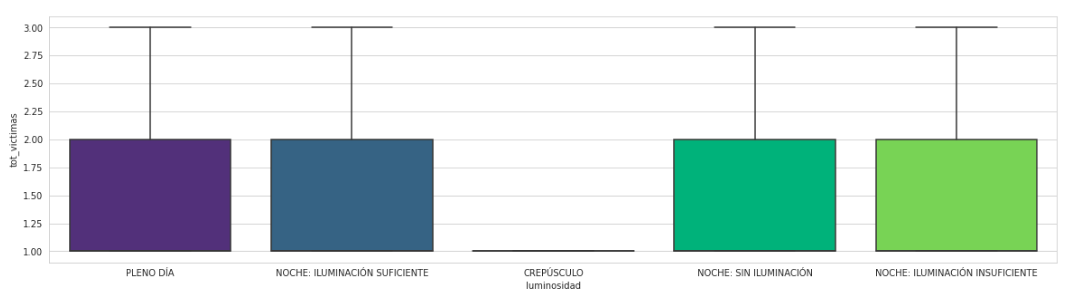
\includegraphics[width=1.1\linewidth]{img/cajas_luminosidad}
	\caption{}
	\label{fig:cajasluminosidad}
\end{figure}

en el que no observamos diferencias en las distribuciones asociadas a las distintas situaciones de luminosidad, salvo el caso del crepúsculo, donde el número de víctimas es 1 prácticamente siempre (menos en los outliers). Para el resto de casos sí hay más dispersión en el número de victimas, pero presentando en cada caso el mismo tipo de distribución.
Los diagramas de barras de las medias de cada atributo en cada situación de luminosidad obtenidos son los siguientes:
\begin{figure}[H]
	\centering
	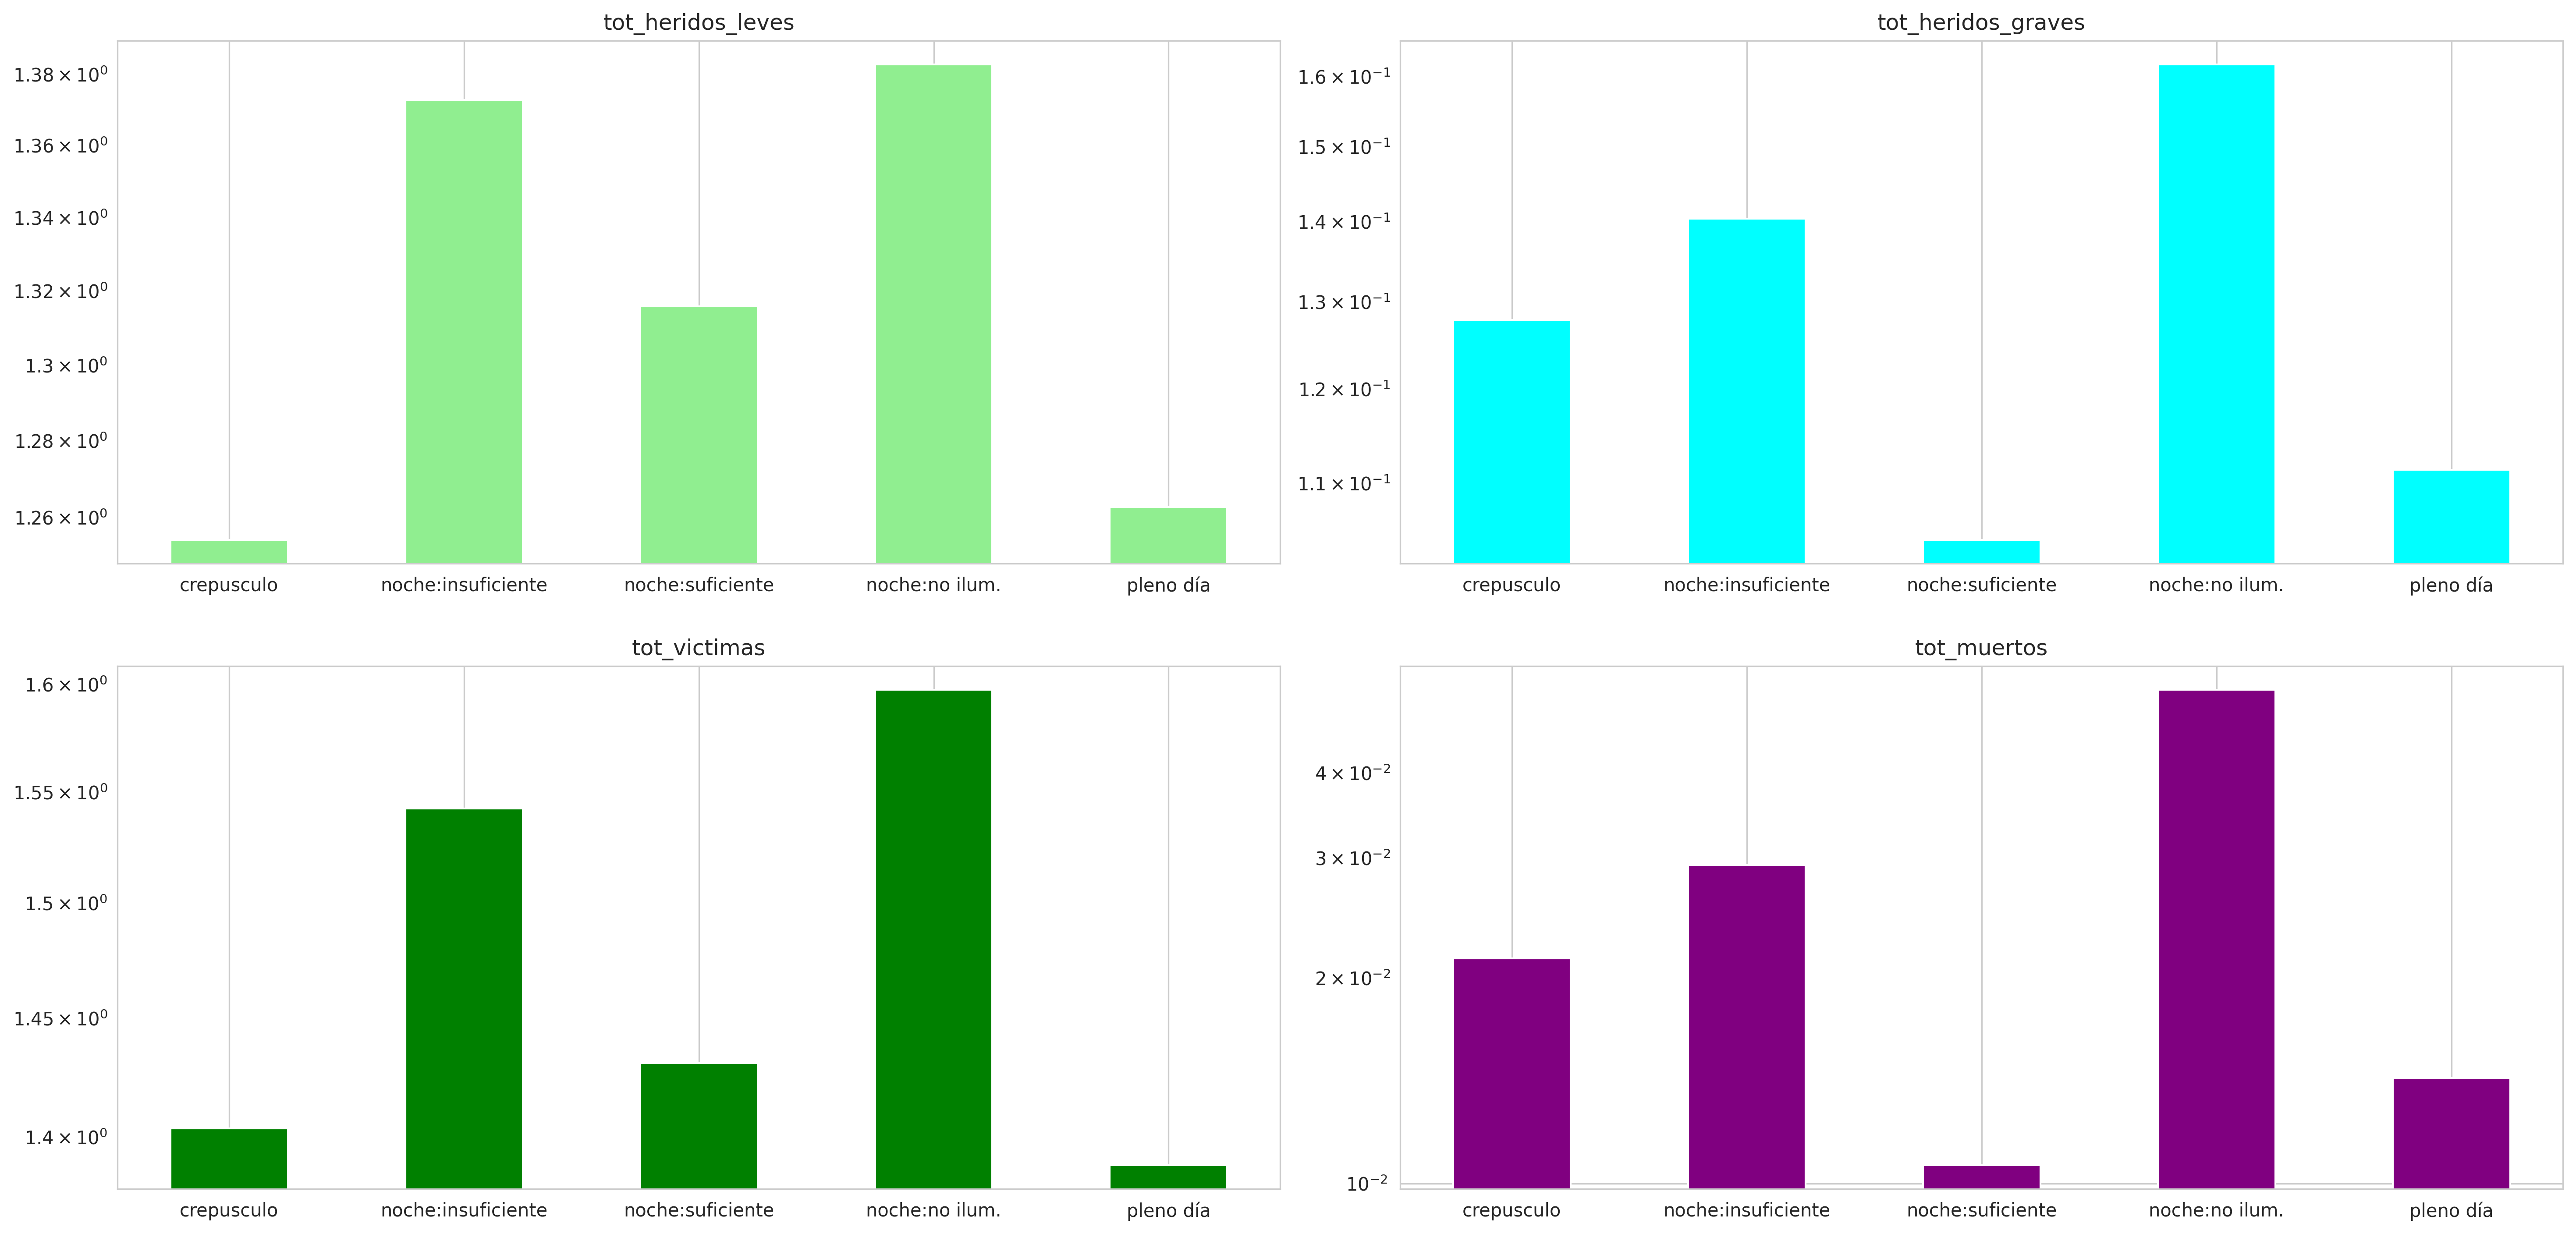
\includegraphics[width=1\linewidth]{img/influencia_luminosidad}
	\caption{}
	\label{fig:influencialuminosidad}
\end{figure}

donde podemos observar que la media de todos los atributos notables es más alta en las noches donde la iluminación es escasa o nula, de acuerdo con la lógica ya comentada. Por ello vamos a analizar el tipo de accidentes que ocurren en estas situaciones de luminosiad.

Además de esta variable, como hemos comentado al principio, vamos a tener en cuenta también el estado de la calzada. Puesto que una calzada helada, mojada o nevada hace más difícil la circulación y las ruedas de los vehículos pueden resbalar con mayor facilidad, es lógico pensar que en estas situaciones tienen lugar más accidentes. Representando el diagrama de cajas 

\begin{figure}[H]
	\centering
	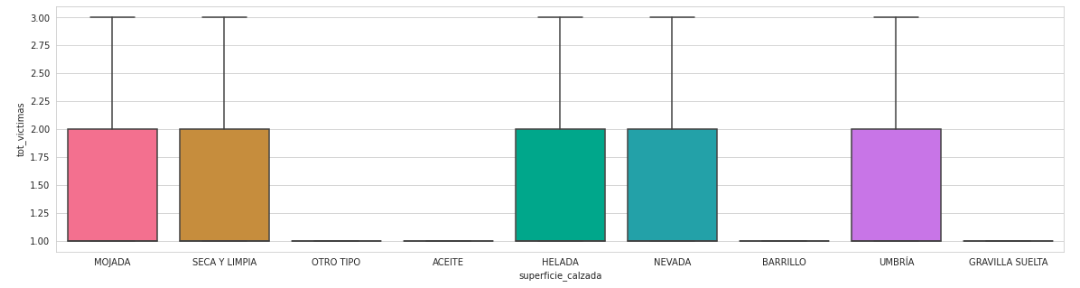
\includegraphics[width=1.1\linewidth]{img/cajas-superficie}
	\caption{}
	\label{fig:cajas-superficie}
\end{figure}

descubrimos que hay dos tipos de distribuciones: unas en las que la mayoría de los datos (todos menos outliers) tienen el mismo número total de víctimas asociadas, a saber, una, y otras en las que la dispersión es mayor, teniendo el 75\% de los datos un número de víctimas menor o igual que dos, el 50\% una única víctima y siendo el valor máximo 3 (sin tener en cuenta los outliers). En este último tipo se encuentran, entre otras, los estados de la calzada que hemos considerado como peligrosos (mojada,helada y nevada), de manera que nuestras sospechas empiezan a confirmarse. En cuanto a los diagramas de barras (obtenidos como en los casos anteriores)
\begin{figure}[H]
	\centering
	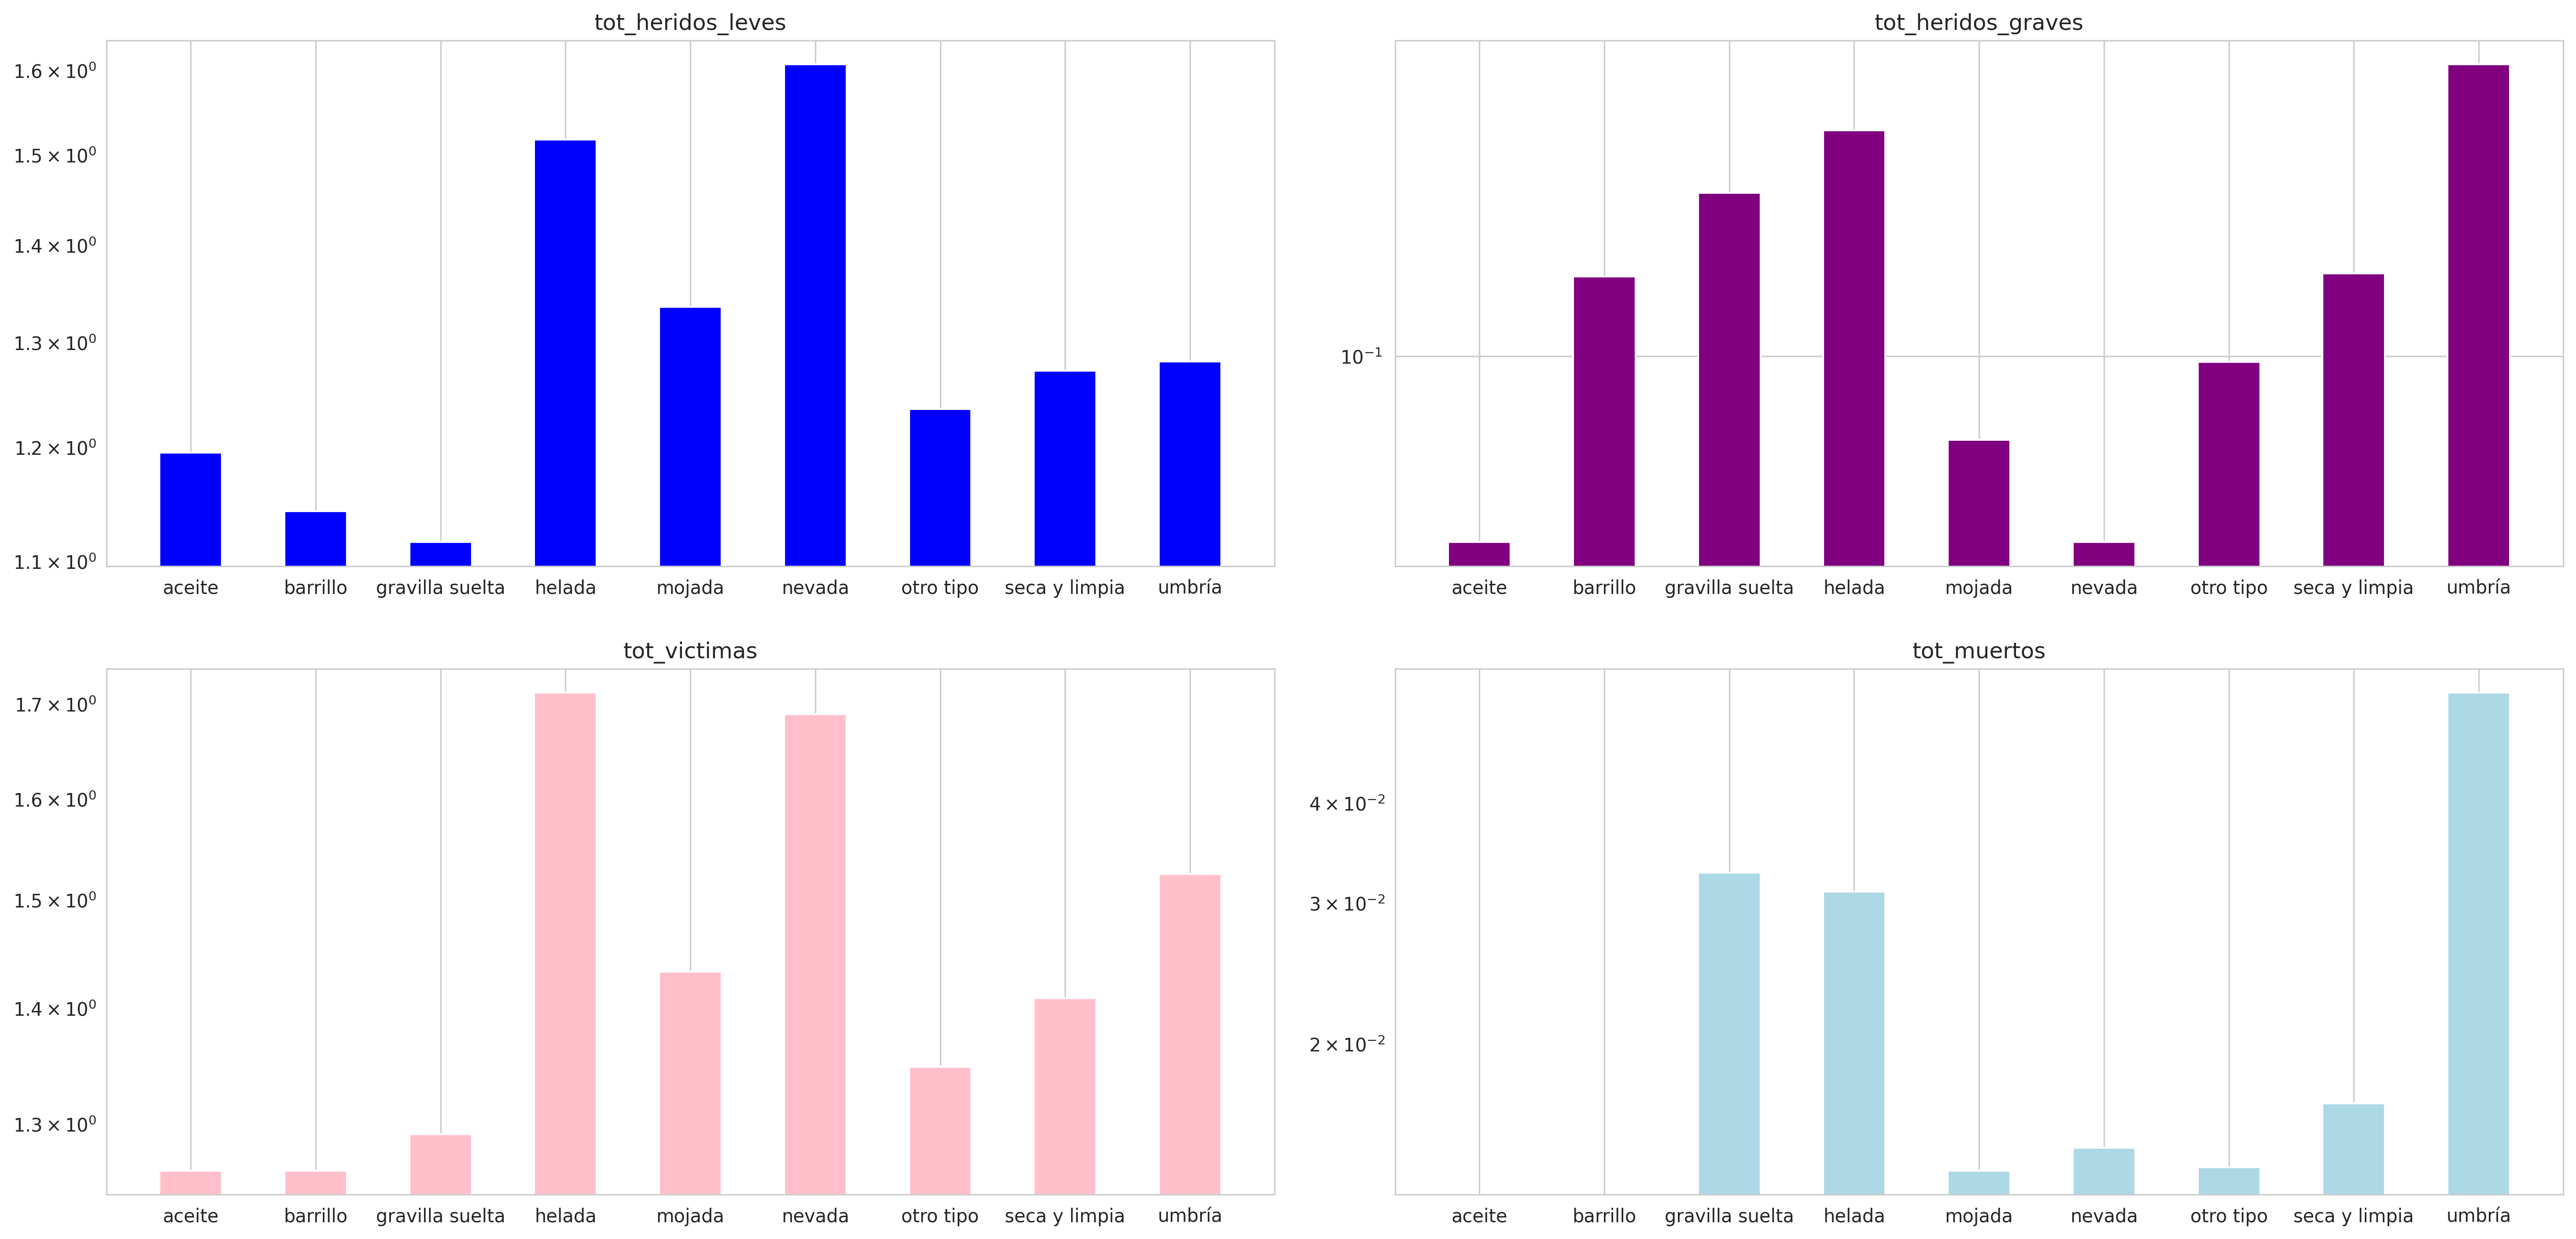
\includegraphics[width=1.1\linewidth]{img/influencia_calzada}
	\caption{}
	\label{fig:influenciacalzada}
\end{figure}
observamos que para el número de víctimas y de heridos leves, los estados de la calzada que hemos considerado muestran el valor de la media más alta, mientras que para los otros atributos los valores difieren y en algunos casos disminuyen, lo cual indica que los accidentes no llegan a ser tan graves en algunas de estas condiciones. Para poder estudiar mejor las diferencias, vamos a aplicar clustering a dichos datos. En el caso de una calzada umbría los resultados son también bastante altos, pero en nuestro estudio no consideraremos esta situación.

En resumen, para este segundo caso de estudio nos vamos a quedar con los accidentes que ocurren bajo condiciones adversas tanto en el sentido de una luminosidad escasa como por el estado de una calzada resbaladiza y poco confiable, e intentaremos analizar los tipos de accidentes que se producen en estas condiciones.

Cómo hicimos en el caso anterior seleccionamos los datos de interés, quedándonos con las instancias del dataset que cumplen las condiciones buscadas y tomando los atributos numéricos relacionados con la gravedad del accidente. Al \mintinline{python}{DataFrame} resultante lo llamaremos ahora \mintinline{python}{caso2}.

\begin{minted}{python}
caso2=raw_data[((raw_data.superficie_calzada == "NEVADA") | 
				(raw_data.superficie_calzada == "MOJADA") |
 				(raw_data.superficie_calzada == "HELADA")) &
 			((raw_data.luminosidad == "NOCHE: ILUMINACIÓN INSUFICIENTE") |
 				 (raw_data.luminosidad == "NOCHE: SIN ILUMINACIÓN"))]
cols=["tot_heridos_leves","tot_heridos_graves","tot_victimas", "tot_muertos",
	"tot_vehiculos_implicados"]
caso2=caso2[cols]

\end{minted}
Convertimos el \mintinline{python}{DataFrame} en una matriz y normalizamos los datos, obteniendo la matriz \mintinline{python}{data_caso2}
\begin{minted}{python}
data_caso2 = to_matrix(caso2, cols)
data_caso2 = norm(data_caso2)
\end{minted}

\subsection{Análisis de los algoritmos}
En este caso vamos a aplicar los algoritmos de Kmeans (nuevamente) y DBSCAN para agrupar los datos, que, como antes, podemos encontrar en \mintinline{python}{sklearn.cluster}.
\subsubsection{K-means}

Vamos a proceder de la misma forma que en el caso de estudio anterior para encontrar el número de clusters óptimo al que aplicar el algoritmo, es decir, haciendo uso del \textit{método del codo} con la medida \textit{distortions}. Usamos entonces la función \mintinline{python}{calcular_k_elbow} con los datos de nuestro estudio normalizados y un rango de número de clusters de entre 2 y 10, obteniendo el siguiente gráfico: 
\vspace{5cm}
\begin{figure}
	\centering
	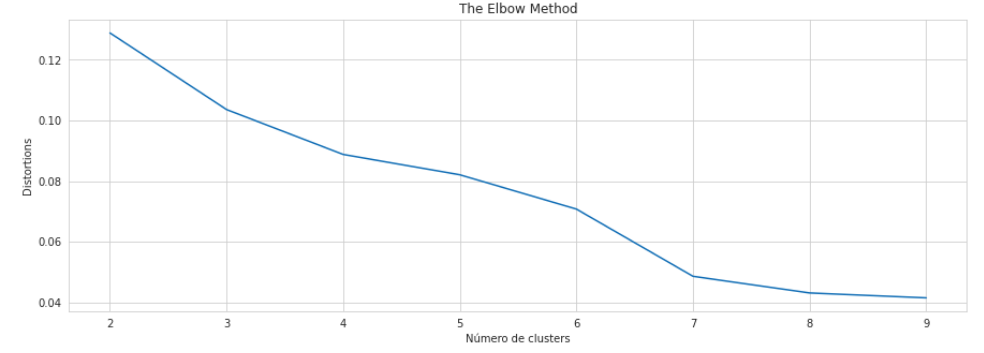
\includegraphics[width=1\linewidth]{img/elbow2}
	\caption{}
	\label{fig:elbow2}
\end{figure}

donde se observa que el 'codo' se encuentra en un número de clusters igual a 7. Corremos entonces la función \mintinline{python}{k_means}, ya explicada, con k=7 y nuestros datos, y los resultados del coeficiente de Silhouette y el índice de Calinski-Harabaz han sido:
\begin{minted}{python}
Silhouette: 0.773931
Calinsky: 1764.636919
\end{minted}

\textbf{Análisis de los clusters obtenidos}\\[0.03cm]

Para analizar los clusters llevamos a cabo las mismas visualizaciones que hemos mostrado hasta ahora. 

El \mintinline{python}{countplot}, que nos indica el número de instancias que contiene cada cluster, ha resultado ser el siguiente:

\begin{figure}[H]
	\centering
	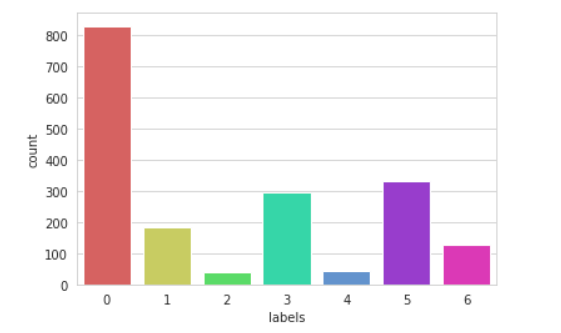
\includegraphics[width=0.7\linewidth]{img/count2}
	\caption{}
	\label{fig:count2-}
\end{figure}

con lo que el cluster 0 es donde se agrupan la mayoría de los datos, conteniendo este unas 800 instancias, seguido por los clusters 5 y 3, que tienen alrededor de 300 datos. Los clusters 2 y 4, con menos de 100 datos, son los más pequeños.

La imagen \mintinline{python}{pairplot} obtenida
\vspace{2cm}
\begin{figure}
	\centering
	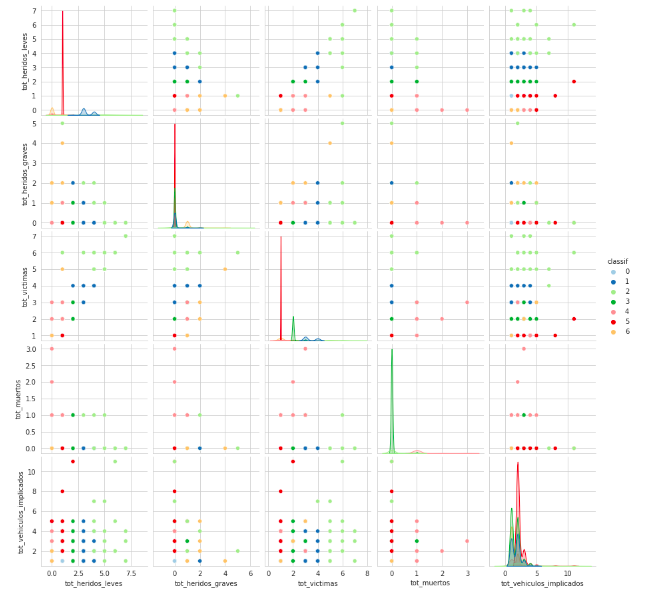
\includegraphics[width=1.1\linewidth]{img/pairplot2}
	\caption{}
	\label{fig:pairplot2}
\end{figure}

no aporta mucha información, salvo que los clusters 2 y 5 son los que más se diferencian del resto de grupos.

A continuación mostramos el mapa de calor y los diagramas de cajas, sin outliers, obtenidos:
\vspace{6cm}
\begin{figure}[H]
	\centering
	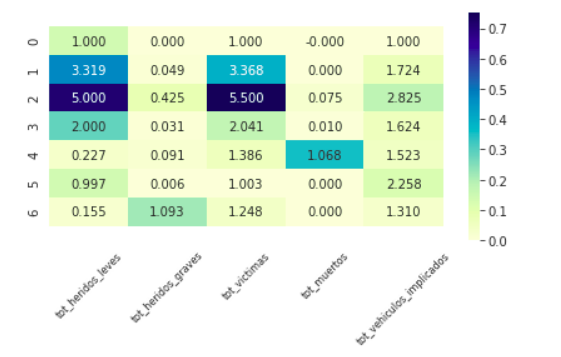
\includegraphics[width=0.9\linewidth]{img/heatmap2}
	\caption{}
	\label{fig:heatmap2}
\end{figure}
\begin{figure}[H]
	\centering
	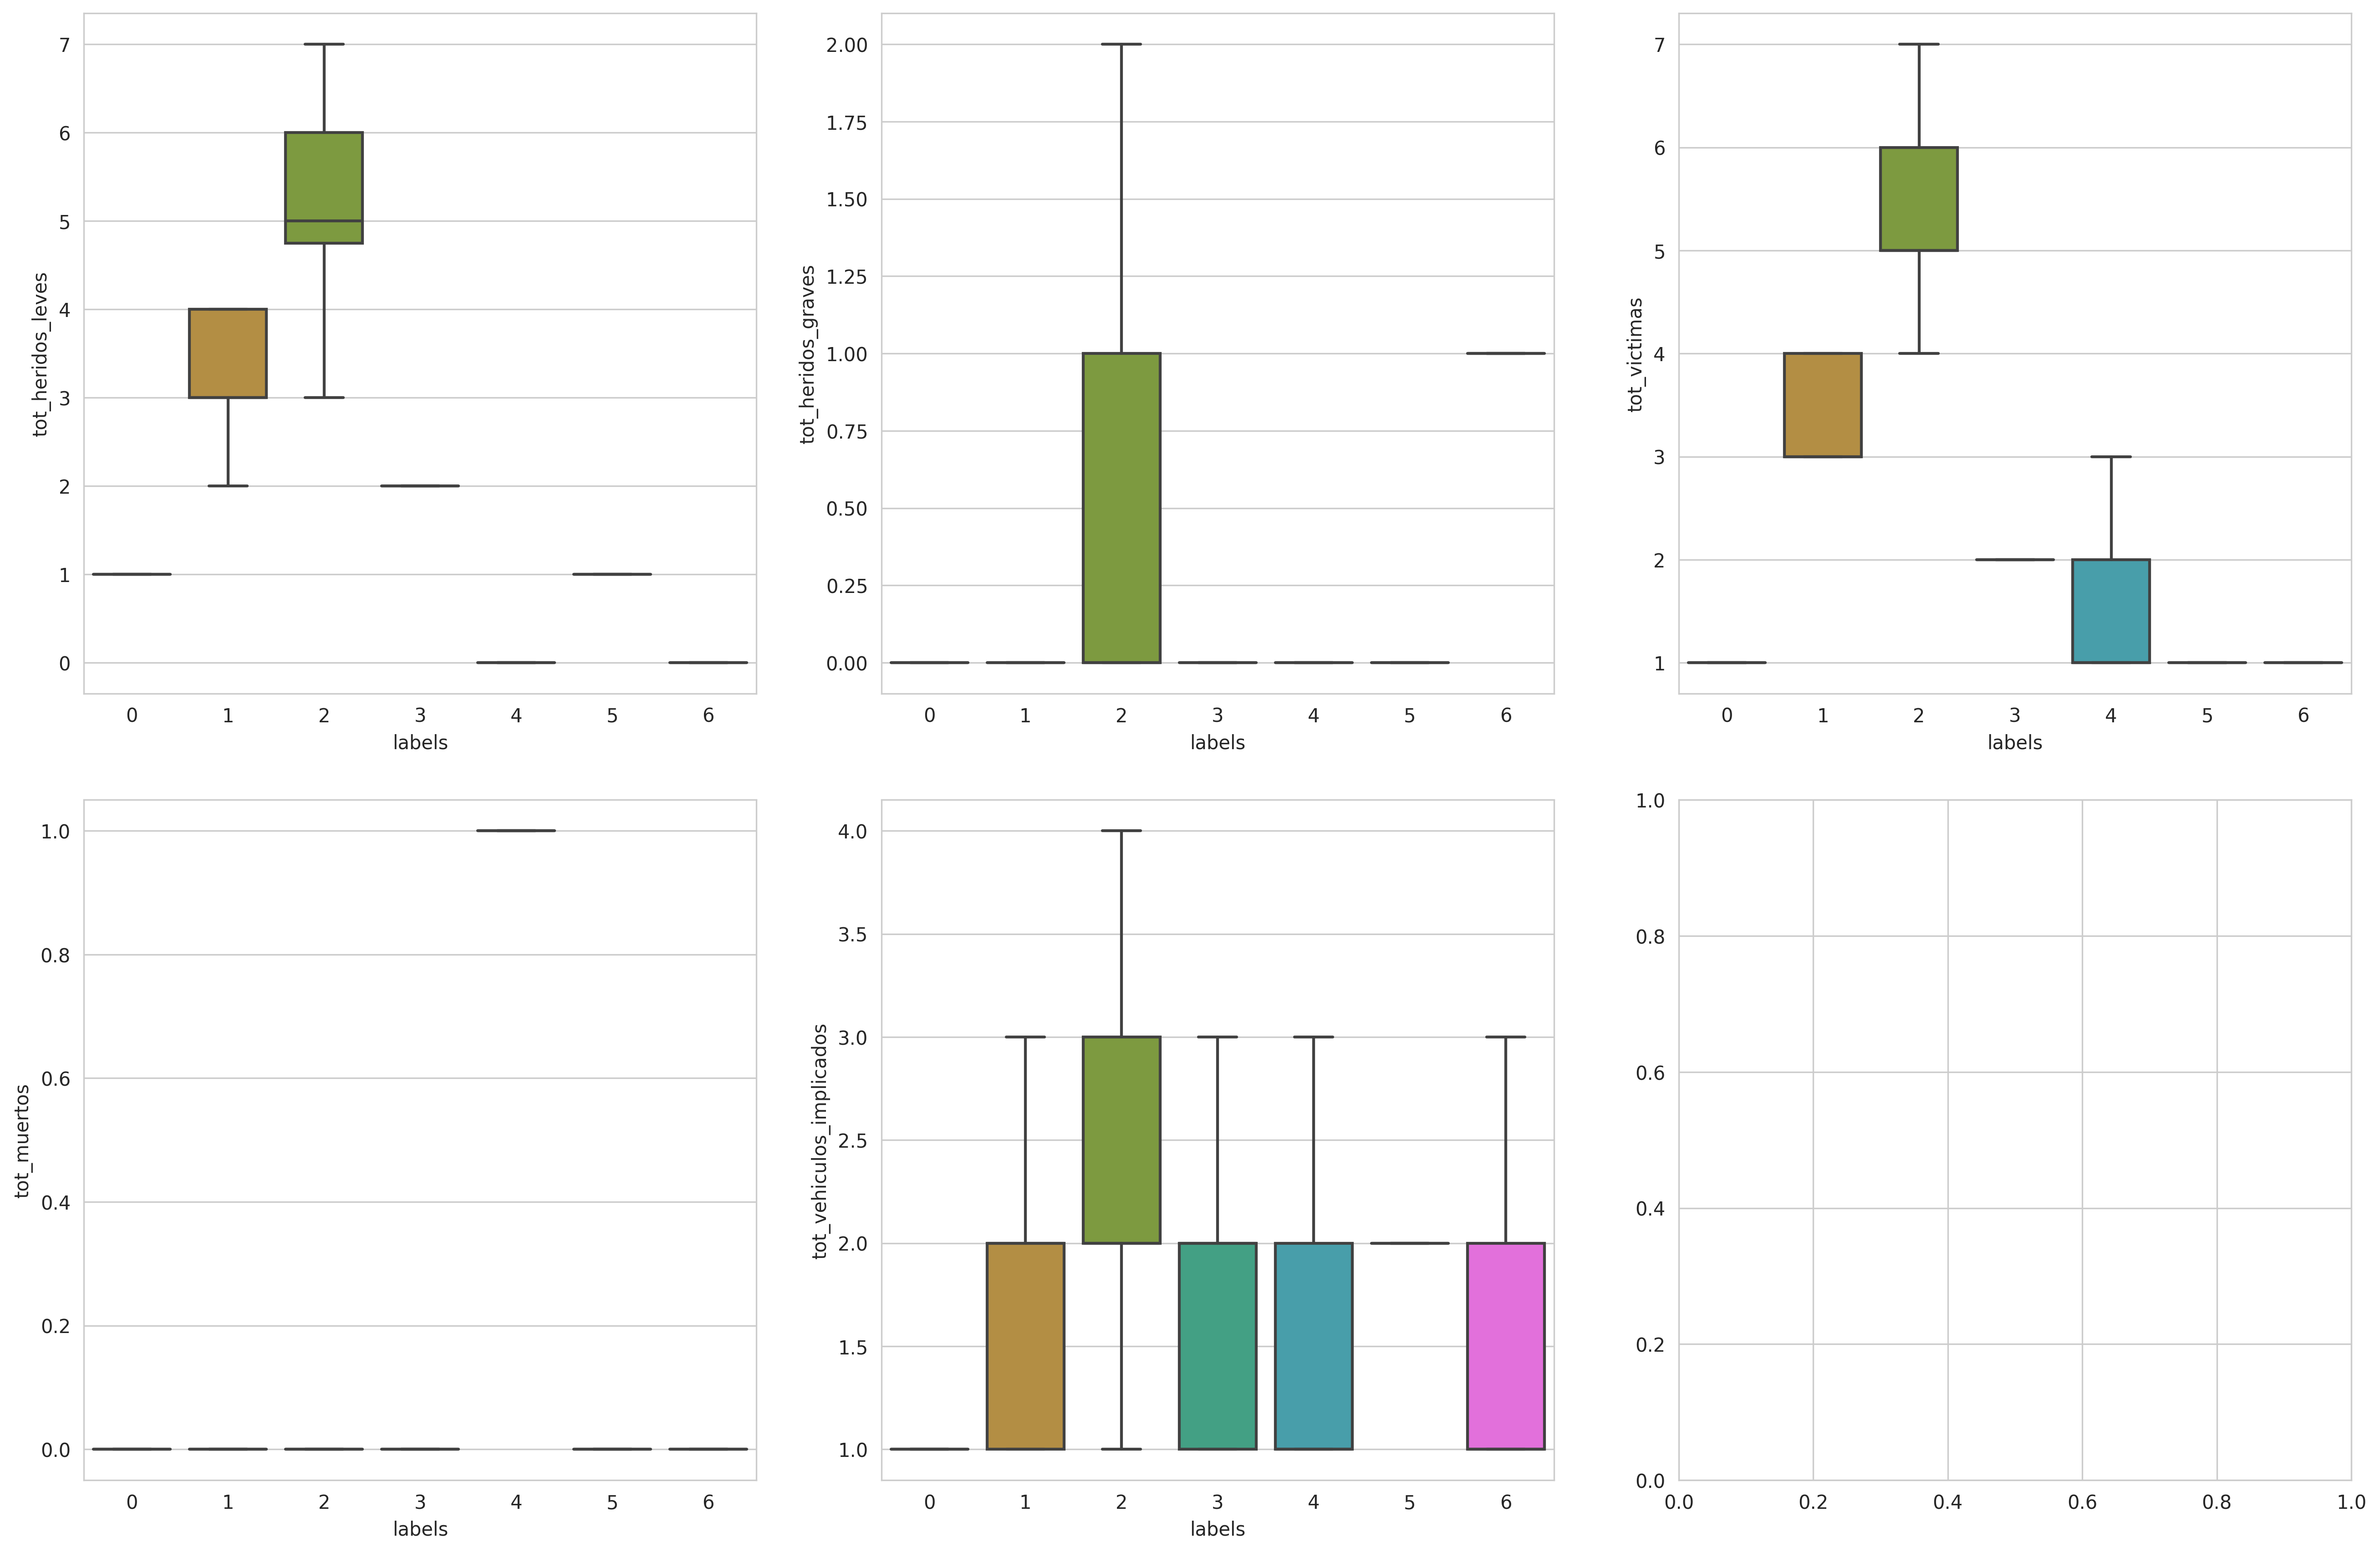
\includegraphics[width=1.1\linewidth]{img/cajas_cluster2}
	\caption{}
	\label{fig:cajascluster2}
\end{figure}

Con todos estos gráficos, nos disponemos ahora a realizar un análisis minucioso de cada uno de los clusters:
\begin{itemize}
	\item A diferencia de lo que ocurrió en el caso de estudio anterior, observamos que aquí sí disponemos de un cluster que recoge los accidentes en los que se han producido algunas muertes. Estamos hablando del \underline{cluster número 4}, en el que la media del número total de muertos es aproximadamente 1 y la distribución es degenerada en 1, por lo que, salvo en algún caso atípico, los accidentes de este cluster están caracterizados por recoger una persona fallecida. Para los otros tipos de víctimas (heridos leves y graves), la distribución es degenerada en 0 con media prácticamente 0, de manera que en este cluster solo se recogen las víctimas que han terminado falleciendo y, por tanto, el número total de víctimas es prácticamente 1 en media y distribución, coincidiendo con el individuo fallecido (salvo algún otro tipo de víctima que se haya colado en este cluster). Por otro lado, el número de vehículos implicados en estos accidentes varía entre 1 y 3, siendo la media 1.5 (pues el 75\% de los datos tienen un valor entre 1 y 2). 
	
	\item Centrándonos en el \underline{cluster número 0}, el que incluye la mayor cantidad de los datos, observamos que se caracteriza por tener un número de heridos leves igual a 1 en todos los casos, que coincide con el número total de víctimas (no hay ni una víctima de otro tipo, ni siquiera outlier, en este cluster). Además, el número total de vehículos implicados siempre es 1 (distribución degenerada en 1 y la media es exactamente 1).
	\item Si prestamos atención ahora al número de heridos graves, nos percatamos de que el cluster que tiene un valor medio más alto para esta variable es el \underline{cluster número 6}. Presenta una distribución degenerada en 1, pero la media es ligeramente superior, por lo que podemos suponer que habá algún outlier aquí que tenga más heridos graves. Se trata, sin embargo, de un número pequeño. Además de este cluster, si nos fijamos en los diagramas de cajas correspondientes a este atributo, podemos observar que el \textit{grupo 2}, también contiene instancias con un número de heridos graves superior a 0, variando este número entre 0 y 2, y con la mitad de los datos presentando entre 0 y 1 heridos graves. Así pues, en este último cluster habrá algunas instancias con 1 o 2 heridos graves, mientras que en el grupo 6 prácticamente todas las instancias contarán con 1 herido grave. 
	
	Si seguimos analizando el cluster 6, tenemos que el número de heridos leves es nulo en todos los casos menos en los outliers, donde este número puede aumentar, lo que lleva a que la media esté algo por encima de 0. El número total de víctimas coincide entonces casi totalmente con el de heridos graves. Por otro lado, la cantidad de vehículos afectados presenta en este grupo una distribución bastante similar a la de la mayoría de los clusters, es decir, como comentamos para el cluster 4, varía entre 1 y 3, estando la mitad de los datos entre 1 y 2, con media algo inferior a la del grupo 4. Así, esta última variable no es representativa de este cluster, pero sí lo es el número de heridos graves. 
	
	\item El \underline{grupo número 2}, además de incluir algún herido grave en ciertos accidentes, se caracteriza por contener los accidentes con el mayor número de heridos leves en nuestro caso de estudio, con una media de 5. La distribución de esta variable presenta un alto grado de dispersión, variando la cantidad entre 3 y 7 heridos, con la mitad de las instancias situadas entre un valor algo inferior a 5 y 6. Lo que queda claro observando los diagramas de cajas de esta variable es que a este cluster pertenecen las instancias que contienen un alto número de heridos leves. En este caso, como la media de heridos graves no es nula, la media y la distribución del número total de víctimas se ve afectada por estos últimos, de manera que presenta valores algo superiores a los de únicamente heridos leves. 
	
	Otra característica de este cluster es que tiene la media de vehículos implicados más alta, pues en la mitad de los accidentes de este grupo intervienen entre 2 y 3 vehículos, llegando incluso en algunos casos a los 4. Es el único grupo en el que la cantidad de vehículos llega a tomar este último valor para algunas instancias. 
	
	\item Para el resto de clusters, podemos destacar que el \underline{cluster número 5} presenta una distribución de los vehículos afectados algo diferente a los demás, pues es degenerada en 2 y su media es aproximadamente 2, de manera que casi todos los datos que contiene incluyen un total de 2 vehículos  (salvo casos atípicos en los que puede ser mayor, pues la media supera el valor 2). Los clusters 1 y 3, tienen la misma distribución para esta variable que la ya comentada para los clusters 4 y 6, con lo que no es un atributo característico de ellos. El resto de atributos en el grupo 5 son prácticamente idénticos a los del cluster 0.
	
	Los \underline{clusters 1 y 3} se caracterizan por tener una media de heridos leves de 3.3 y 2 respectivamente, siendo la segunda distribución degenerada en 2 y la primera algo más dispersa, con la mitad de los datos presentando entre 3 y 4 heridos y siendo el mínimo 2. El número de víctimas en ambos casos viene caracterizado por el número de heridos leves, ya que no hay heridos graves ni muertos en ninguno de los grupos. 
\end{itemize}

\textbf{Resumen:}
\begin{itemize}
	\item [--] La mayoría de los accidentes, agrupados en el cluster 0, presentan un único herido leve correspondiente a un solo vehículo implicado.
	\item [--] En otra gran parte de los datos (cluster 5), el número de heridos leves es también uno, pero con un total de vehículos afectados de 2. 
	\item [--] En los siguientes tipos de accidentes más usuales de nuestro estudio intervienen 1 o 2 vehículos, siendo el número de heridos leves más frecuente de 2 (cluster 3), seguido por 3 (cluster 1). 
	\item [--] Puede ocurrir también que alguien salga herido gravemente (cluster 6) con 1 o 2 vehículos implicados, pero esta situación es menos usual que las anteriores. 
	\item [--] En una mínima parte de las situaciones (cluster 2), hay más vehículos afectados, entre 2 y 3 e incluso a veces 4, y, en consecuencia, un mayor número de heridos, entre 5 y 6 leves y 1 o 2 graves.
	\item [--] Raramente alguien puede fallecer en estos accidentes (cluster 4), cuando los vehículos implicados son 1 o 2. 
\end{itemize}

\subsubsection{Algoritmo DBSCAN}
Estudiamos ahora los resultados obtenidos con el algoritmo DBSCAN. Se trata de un algoritmo basado en densidad que separa regiones con una alta densidad de datos de regiones con una densidad más baja. Los clusters son vistos por este algoritmo como regiones de alta densidad separados por áreas de menor densidad de datos. El número final de clusters es determinado automáticamente por el algoritmo, al contrario de lo que ocurría en K-means. Además, puede encontrar clusters de cualquier forma, no solo convexos, y es capaz de identificar los outliers fácilmente. Sin embargo, no trabaja bien con clusters de densidad variable o con conjuntos de datos muy dispersos. 

Dos parámetros son clave para determinar el concepto de densidad.  Por un lado necesitamos fijar un valor para \mintinline{python}{epsilon}, que es la distancia máxima entre dos puntos para que sean considerados 'vecinos', es decir, pertenecientes al mismo cluster. Cuanto menor sea dicho valor, mayor será la densidad necesaria para formar un cluster. Se trata de un parámetro crucial que determina la 'vecindad' local de los datos.  Si se elige un valor muy grande  puede ocurrir que clusters vecinos se mezclen dando lugar a un único cluster, cuando en realidad formarían dos clusters diferentes, y si se escoge muy pequeño muchos datos pueden quedarse fuera de su cluster correspondiente y ser clasificados como outliers.  Por otro lado tenemos \mintinline{python}{min_samples}, que define el número mínimo de puntos vecinos que debe tener un punto concreto para ser considerado como un punto central del cluster, incluyendo al propio punto. Un valor alto de este parámetro implica que la densidad de cada cluster será mayor. Controla básicamente cómo de tolerante es el algoritmo ante el ruido. Como se indica en el enlace \cite{13}, este valor debe escogerse igual o mayor al número de dimensiones + 1, por lo que nosotros lo fijamos a 6. No vamos a centrarnos entonces en buscar el valor óptimo de este último parámetro, sino del primero, pues ya hemos comentado que es más importante.

Para buscar el valor más adecuado de \mintinline{python}{epsilon} usamos ahora el coeficiente de \underline{Silhouette} y el índice de \underline{Calinski-Harabaz}, de manera que el valor de épsilon que nos de un coeficiente de Silhouette más cercano a 1 y un índice de Calinski-Harabaz más alto será el mejor para usar en el algoritmo. Por lo tanto, vamos a implementar una función que aplique el algoritmo para un cierto rango de valores de epsilon, almacene en cada caso los resultados de los dos coeficientes considerados y los muestre gráficamente. Dicha función quedaría como sigue: 

\begin{minted}{python}
def calcular_eps(data,num,eps_min,eps_max):
	costs=[[] for i in range(2)] 
	for n in np.linspace(eps_min, eps_max, num=num):
	resultado = DBSCAN(min_samples=6,eps=n).fit(data)
	
	silhouette, calinski = measures_silhoutte_calinski(data, resultado.labels_)
	
	costs[0].append(silhouette)
	costs[1].append(calinski)
	
	fig, (ax1, ax2) =plt.subplots(1,2,figsize=(15,5))
	ax1.plot(np.linspace(eps_min, eps_max, num=num), costs[0])
	ax1.set_xlabel('eps')
	ax1.set_ylabel('Silhouette')
	
	ax2.plot(np.linspace(eps_min, eps_max, num=num), costs[1])
	ax2.set_xlabel('eps')
	ax2.set_ylabel('Calinski')
	plt.show()
\end{minted}

donde \mintinline{python}{eps_min} y \mintinline{python}{eps_max} indican el valor mínimo y máximo de epsilon a considerar, respectivamente, y \mintinline{python}{num} es el número de valores diferentes de epsilon en el rango considerado con los que queremos probar. Si ejecutamos ahora 
\begin{minted}{python}
calcular_eps(data_caso2,30,0.005,0.25)
\end{minted}
obtenemos la siguiente salida: 
\begin{figure}[H]
	\centering
	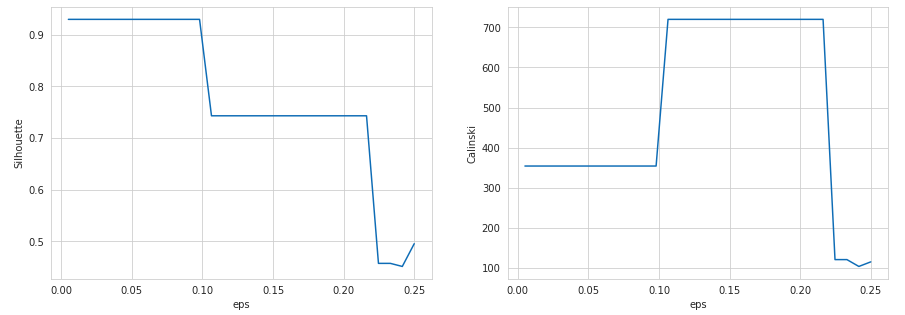
\includegraphics[width=1.1\linewidth]{img/epsilon1}
	\caption{}
	\label{fig:epsilon1}
\end{figure}
donde podemos observar que cuando el coeficiente de Silohuette empieza a decrecer es cuando el índice de Calinski aumenta. Esta región crítica se encuentra en torno a $eps=0.1$, por lo que vamos a enfocarnos en ella ejecutando:
\begin{minted}{python}
calcular_eps(data_caso2,30,0.095,0.105)
\end{minted}
y obtenemos así: 
\begin{figure}[H]
	\centering
	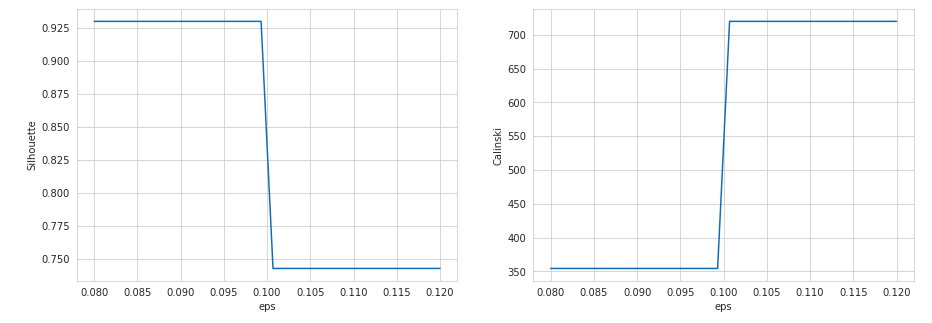
\includegraphics[width=1.1\linewidth]{img/epsilon2}
	\caption{}
	\label{fig:epsilon2}
\end{figure}



Para que ninguno de los dos coeficientes sea especialmente bajo, vamos a considerar un término medio entre ambos, con lo que seleccionamos $epsilon=0.1$, que es justo cuando se produce el cambio. 

Una vez que hemos decidido el valor del parámetro \mintinline{python}{epsilon} con el que vamos a trabajar, procedemos a ejecutar el propio algoritmo con dicho valor del parámetro y a analizar los resultados obtenidos. Para ello implementamos otra función que llama al algoritmo \textbf{DBSCAN}, muestra los valores de los coeficientes de Silhouette y Calinski-Harabaz y devuelve el resultado de aplicar el algoritmo a los datos pasados como parámetro con un valor de \mintinline{python}{eps=n}:
\begin{minted}{python}
def dbscan(data,n):
	resultado = DBSCAN(min_samples=6,eps=n).fit(data)
	
	silhouette, calinski = measures_silhoutte_calinski(data, resultado.labels_)
	
	print("Silhouette: {:3f}".format(silhouette))
	print("Calinsky: {:3f}".format(calinski))
	
	
	return resultado
\end{minted}

Ejecutando la función:
\begin{minted}{python}
	resultado_db=dbscan(data_caso2,0.1)
\end{minted}

tenemos la siguiente salida:

\begin{minted}{python}
	Silhouette: 0.743859
	Calinsky: 692.085703
\end{minted}

\textbf{Análisis de los clusters obtenidos}

Pasamos ahora a analizar los clusters que resultan tras aplicar el algoritmo DBSCAN a partir de varias visualizaciones. En este caso no vamos a considerar la imagen \mintinline{python}{pairplot}, pues si ya aportaba poca información en los casos anteriores, aquí con un total de  13 clusters e incluyendo uno especial que contiene los outliers y que, por lo tanto, es de gran dispersión, la información que podemos sacar de ella es prácticamente nula. 

La primera de las visualizaciones consideradas es un \mintinline{python}{countplot}:
\begin{figure}[H]
	\centering
	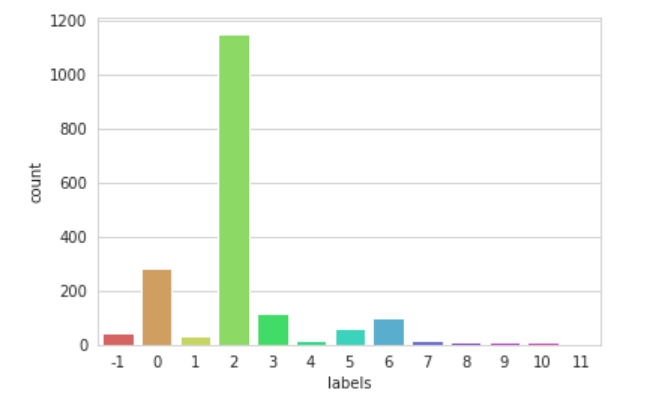
\includegraphics[width=0.9\linewidth]{img/count5}
	\caption{}
	\label{fig:count5}
\end{figure}


Podemos observar que se han generado 13 clusters, incluyendo el cluster etiquetado como -1, en el que se recogen los datos que el algoritmo ha detectado como outliers. Algunos de estos grupos de datos contienen muy pocas instancias (menos de 50), siendo el cluster número 11 prácticamente inexistente. De esta forma nos vamos a centrar en los clusters que tienen un mayor número de datos, es decir, los clusters número 0, 2, 3, 5 y 6. El cluster número 1 tiene también un tamaño muy pequeño, pero es ligeramente superiar al de los otros clusters que no vamos a considerar (clusters 4,7,8,9, 10 y 11), con lo que también vamos a tenerlo en cuenta. El grupo de los outliers no tiene interés y vamos a ignorarlo. 

La mayoría de los datos se agrupan en el cluster número 2, el cual contiene más de 1000 datos. El siguiente cluster más grande es el número 0, aunque la diferencia de tamaño con el primero es enorme, pues se diferencian en alrededor de 800 datos. Los clusters número 3 y 6 tienen en torno a 100 datos cada uno, siendo el primero ligeramente mayor que el segundo.  Finalmente, nos encontramos con los clusters 5 y 1, que son los más pequeños y recogen algunas decenas de datos. El cluster 5 es algo mayor que el 1, pero la diferencia es mínima. 

Veamos ahora el mapa de calor de los centros de cada cluster (donde el cluster número 0 es el cluster -1 y entonces el resto de etiquetas están cambiadas de manera que cada número corresponde al cluster etiquetado con un número menos): 
\begin{figure}[H]
	\centering
	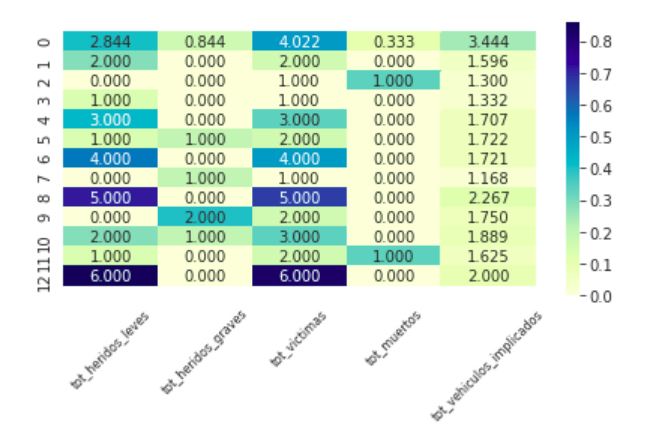
\includegraphics[width=0.8\linewidth]{img/heatmap5}
	\caption{}
	\label{fig:heatmap5}
\end{figure}
y los diagramas de cajas asociados a los distintos atributos considerados: \\[5cm]
\begin{figure}[H]
	\centering
	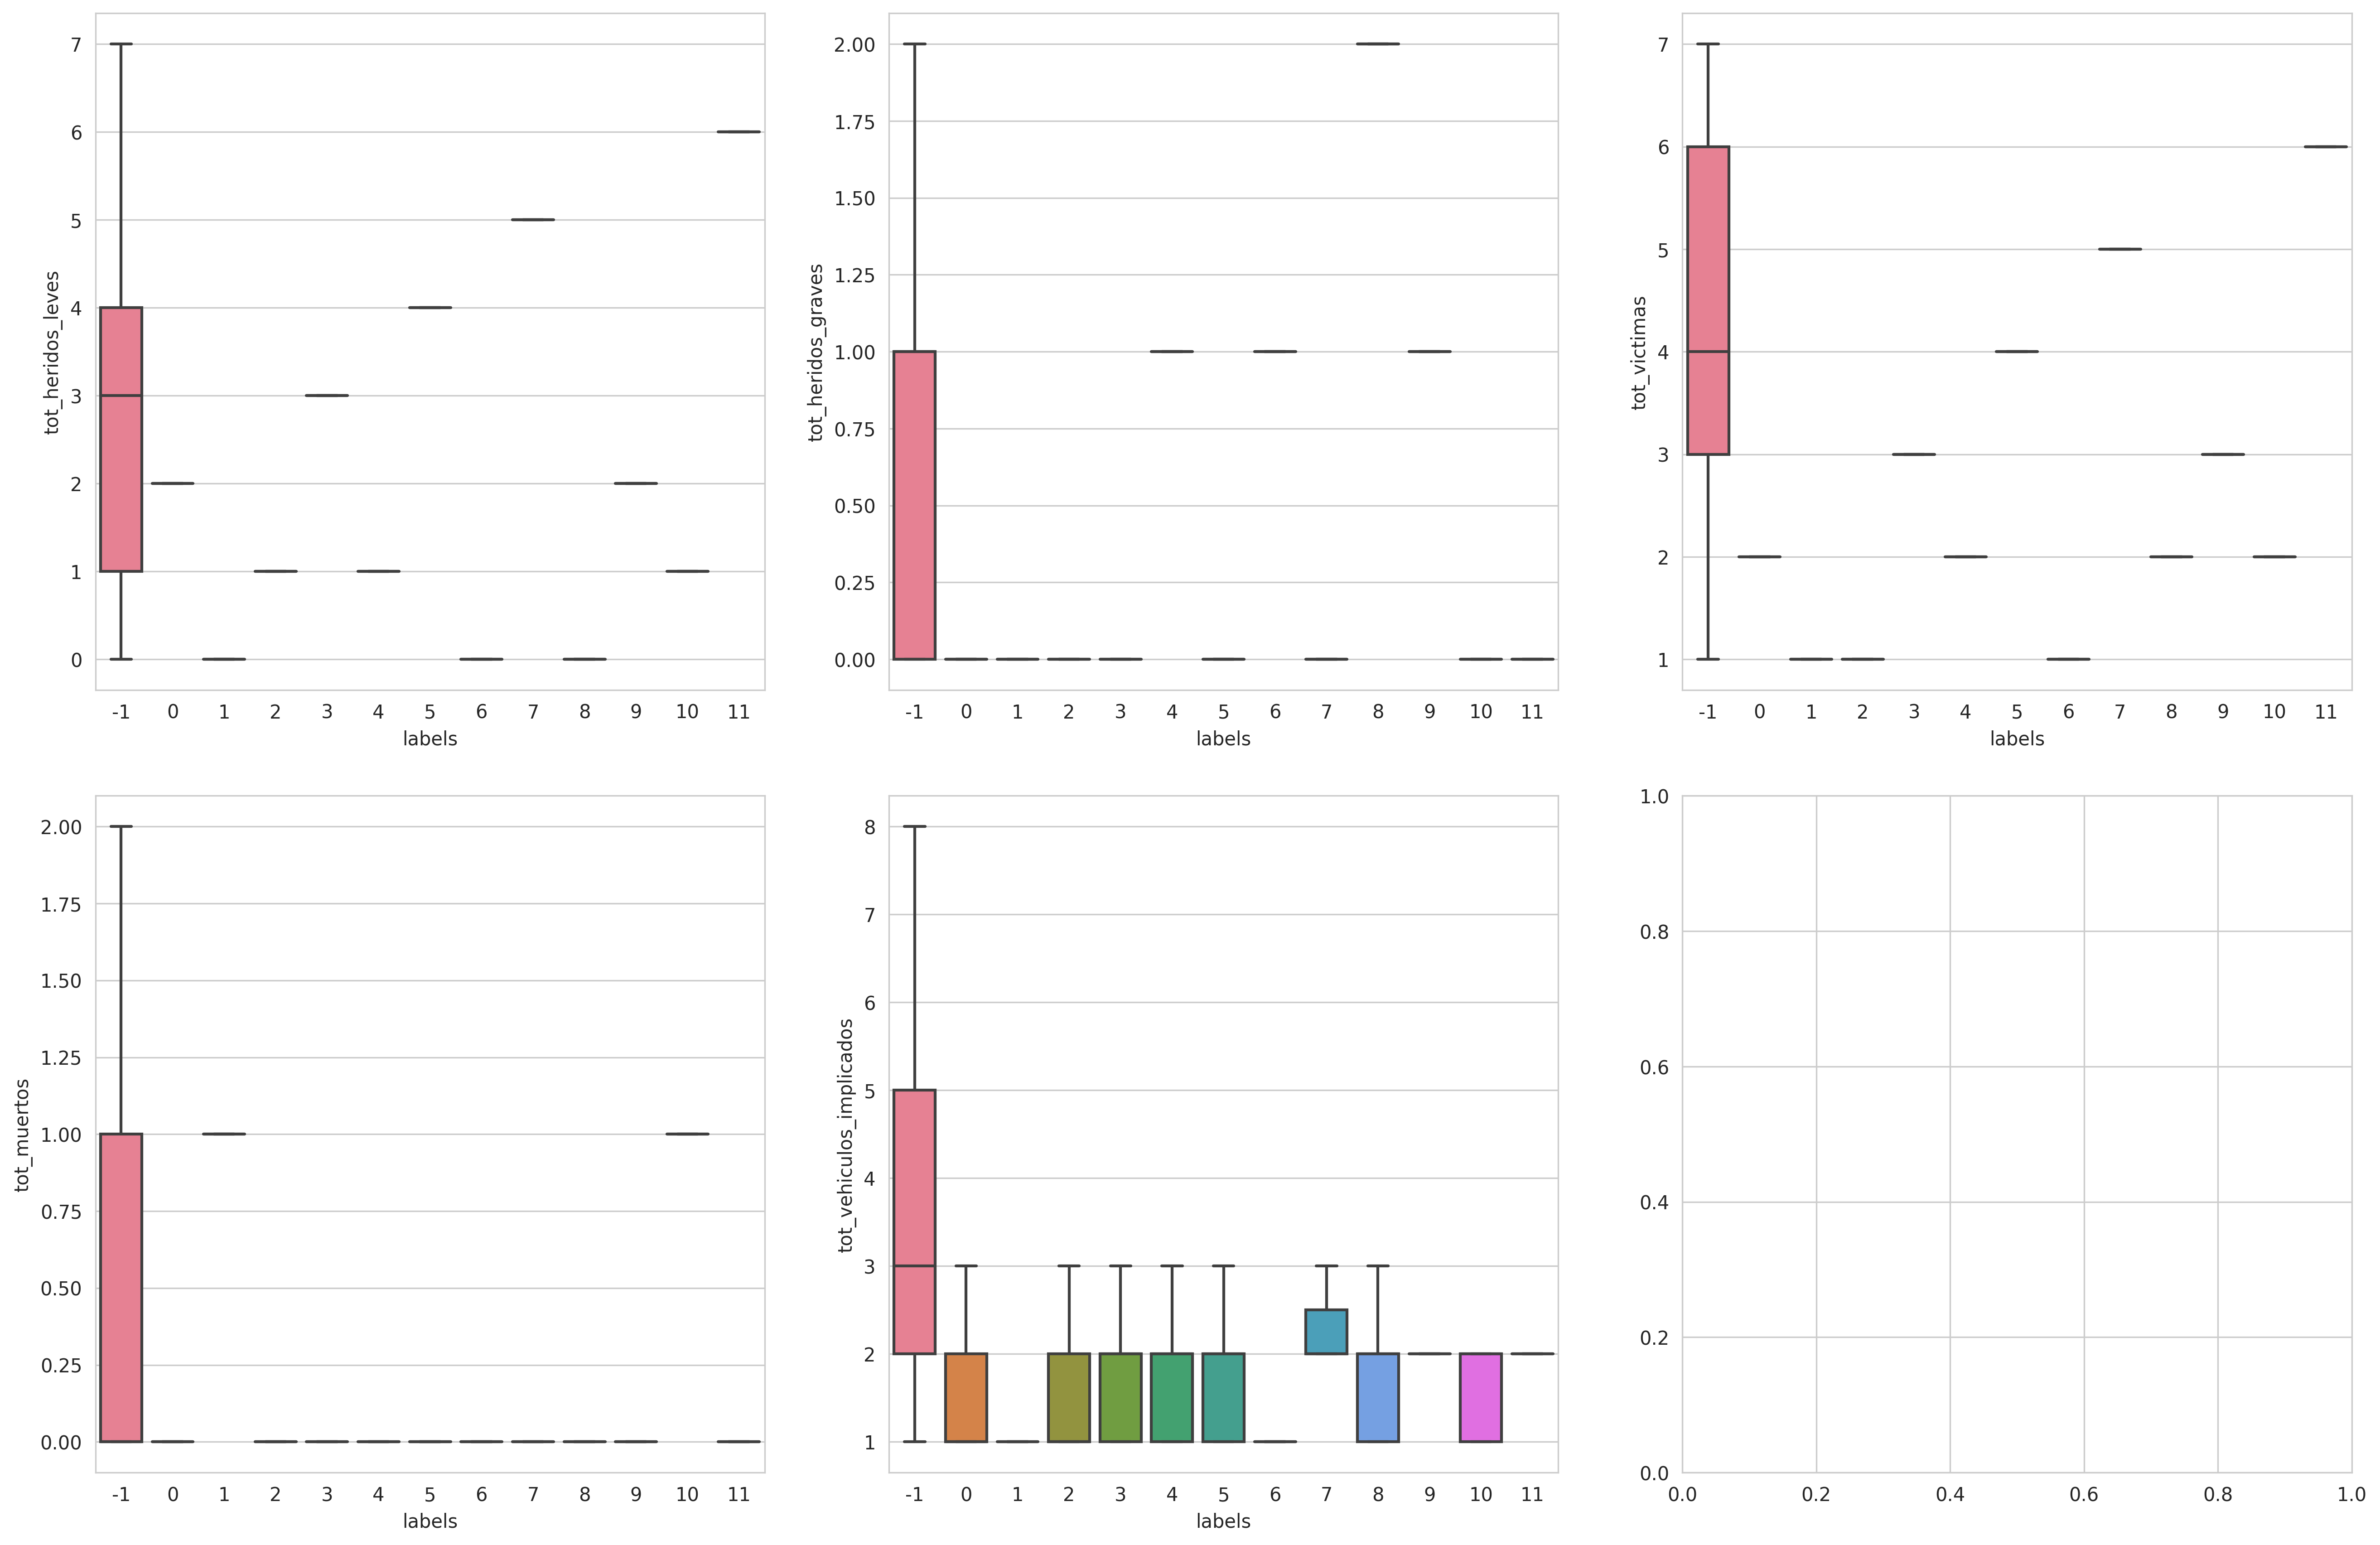
\includegraphics[width=1.1\linewidth]{img/cajas_cluster5}
	\caption{}
	\label{fig:cajascluster5}
\end{figure}

Basándonos en todos estos gráficos comentamos ahora los aspectos más destacables de los clusters considerados:
\begin{itemize}
	\item[-] En todos los clusters el número de vehículos implicados varía entre 1 y 3, siendo 1 o 2 los valores más comunes.
	\item[-] La mayoría de los accidentes, agrupados en el cluster 2, presentan un único herido leve, y otra gran parte de los datos, correspondiente al cluster 0, son accidentes en los que resultan 2 heridos leves.
	\item [-] Encontramos también algunos datos en los que el número de heridos leves asciende a 3 (cluster 3), o incluso a 4 (cluster 5), aunque estos suponen una menor proporción que los accidentes anteriores. 
	\item [-] El cluster número 6 agrupa en torno a 100 accidentes, en los que alguien resulta herido gravemente.
	\item [-] Finalmente tenemos algunas decenas de datos donde aperece un fallecido, que se recogen en el cluster número 1. 
\end{itemize}


\newpage
\subsubsection{Comparación de ambos algoritmos}
Comparamos ahora los resultados proporcionados por cada uno de los algoritmos considerados. 

El coeficiente de Silhouette y el índice de Calinski-Harabaz resultantes en cada caso han sido los siguientes:

\begin{table}[htbp]
	\caption{}
	\begin{center}
		\begin{tabular}{|c|r|r|}
			\hline
			\textbf{} & \multicolumn{1}{c|}{\textbf{K-Means}} & \multicolumn{1}{c|}{\textbf{DBSCAN}} \\ \hline
			Silhouette:  & 0.773931 & 0.743859 \\ \hline
			Calinsky:  & 1764.636919 & 692.085703 \\ \hline
	\end{tabular}\end{center}
	\label{}
\end{table}

donde nos damos cuenta de que el algoritmo de K-means presenta los mejores resultados, tanto para el coeficiente de Silhouette, puesto que este es más cercano a 1, como para el índice de Calinski-Harabaz, siendo la diferencia de este último entre ambos algoritmos bastante grande. Es más, si nos fijamos en la Figura 2.24 podemos observar que lo máximo que llega a valer este índice en el algoritmo de DBSCAN es algo más de 700, mientras que para el algoritmo de K-means está en 1794.64. Por la tanto, podemos decir que según estas métricas el algoritmo de K-means es mejor en este segundo caso de estudio. 

A esta misma conclusión podemos llegar analizando los cluster obtenidos con cada uno de los algoritmos. Mientras que todos los grupos que nos ofrecía K-means tenían un número de instancias considerable y presentaban características bien definidas que permitían diferenciar entre los distintos clusters, con el algoritmo DBSCAN obteníamos clusters con un número de instancias muy pequeño que a penas podrían considerarse como clusters propios. Es decir, este último algoritmo incurría en un sobreajuste, problema que no se presentaba en el primero, de ahí que los resultados sean mejores con K-means que con DBSCAN. Un punto positivo que podemos mencionar del último es que consigue detectar los outliers y no incluirlos en los grupos que no le corresponden, lo cual no tenía en cuenta el primero y aparecían outliers en grupos a los que no pertenecían. 


\newpage
\subsection{Interpretación de la segmentación}
Una vez analizados los clusters resultantes tras aplicar cada uno de los dos algoritmos considerados en este caso de estudio, vamos a intentar interpretar los resultados. Los clusters obtenidos con el algoritmo de DBSCAN  que estudiamos (excluyendo los que apenas tenían datos) eran bastante similares a los que nos ofrecía el algoritmo de K-means.

En las concidiones seleccionadas, esto es, cuando la calzada está nevada, mojada o helada, es más probable que las ruedas resbalen, y el vehículo termine saliendo de la vía, cambiando de dirección, etc, y en definitiva, teniendo un accidente. Por la noche y con la calzada en estos estados, salvo que sea estrictamente necesario por urgencia o trabajo, la gente suele desplazarse menos, por lo que el número de vehículos en la vía es generalmente bastante bajo. Esto explica el hecho de que el número de vehículos afectados sea 1 en casi todos los casos, pues coincide con el vehículo que resbala o tiene problemas por cualquier otro motivo, que se encuentra prácticamente solo en la vía y es raro que choque contra otro vehículo. En algunas situaciones sí puede ser que se vean afectados un par de vehículos, pero, en cualquier caso, que esta cantidad supere el 2 es poco frecuente, de ahí que los accidentes con más de 2 vehículos implicados constituyan una minoría. 

La mayor parte de los datos de nuestro caso de estudio presenta un único herido leve, pues coincidirá con el propio conductor del vehículo implicado. También podemos encontrar instancias con 2 o 3 heridos leves, que podrían ser los conductores de los otros vehículos (si intervienen dos o tres) o los acompañantes del/los conductor/es afectado/s. Es muy poco probable que en nuestros accidentes resulten más de 3 personas heridas, puesto que, como ya hemos comentado, en estas condiciones no suelen viajar muchas personas y, en consecuencia, lo normal es que en un vehículo no vayan muchas personas juntas. El hecho de que el número de vehículos implicados no suela ser mayor de 2 también implica que el número de heridos no sea elevado por lo general. 

Por otro lado, encontramos personas fallecidas sólo en algunas decenas de instancias, siendo el número de decesos 1 en cada uno de estos casos, que coincidirán con accidentes más graves, los cuales tienen lugar de manera mucho menos frecuente en general, de ahí que en muy pocas instancias de los datos de que disponemos aparezcan muertos (en total un $1348/89519=0.015$, es decir, un $1,5\%$ de nuestro dataset presentan víctimas mortales). El hecho de que en nuestro estudio tengamos algunas decenas es, por tanto, considerable. Como estamos estudiando situaciones adversas, sin iluminación y con calzada resbaladiza, era esperable encontrarnos con algunos fallecidos. 

Además, obtuvimos con ambos algoritmos un cluster que contenía accidentes en los que había un herido grave. Este grupo de datos no era muy grande, pero tenía un tamaño considerable y mayor que el de otros clusters. Al igual que ocurre con los fallecidos, encontrar accidentes con heridos graves es poco frecuente, con lo que, ya que aparecen bastantes datos con heridos graves, podemos decir que bajo las condiciones adversas que aquí hemos considerado es más probable de lo normal que alguien termine herido gravemente. En los casos en los que hay heridos graves estos son normalmente sólo 1, pues coincidirá con el conductor del vehículo que tuvo problemas.
\newpage
\section{Caso de estudio 3}
Este caso de estudio es un poco diferente a los anteriores, pues lo que vamos a hacer aquí es considerar los accidentes que se produjeron cuando había suficiente iluminación y la calzada estaba mojada, helada o nevada, para poder comparar los tipos de accidentes que tienen lugar bajo estas ciscunstancias con los obtenidos en el caso de estudio 2. 

Para ello, como hemos hecho en los dos casos de estudio anteriores, nos quedamos con los datos y las variables del dataset que nos interesan para nuestro estudio y al conjunto de datos resultante lo llamamos \mintinline{python}{caso3}:
\begin{minted}{python}
	caso3=raw_data[((raw_data.superficie_calzada == "NEVADA") |
	 (raw_data.superficie_calzada == "MOJADA") | 
	 (raw_data.superficie_calzada == "HELADA")) &
	  ((raw_data.luminosidad != "NOCHE: ILUMINACIÓN INSUFICIENTE") 
	  & (raw_data.luminosidad != "NOCHE: SIN ILUMINACIÓN"))]
	caso3=caso3[cols]
\end{minted}

Pasamos este DataFrame a una matriz, normalizamos sus entradas y al resultado lo denominamos \mintinline{python}{data_caso3}:
\begin{minted}{python}
	data_caso3 = to_matrix(caso3, cols)
	data_caso3 = norm(data_caso3)
\end{minted}
\subsection{Análisis de los algoritmos}
Para llevar a cabo la segmentación nos centramos en  este caso únicamente en el algoritmo de K-means, pues es el que nos ofreció mejores resultados en los casos de estudio anteriores. 

Aplicando el método del codo a los datos de nuestro caso de estudio y un rango de número de clusters de entre 2 y 10, obtenemos lo siguiente: 
\begin{figure}[h]
	\centering
	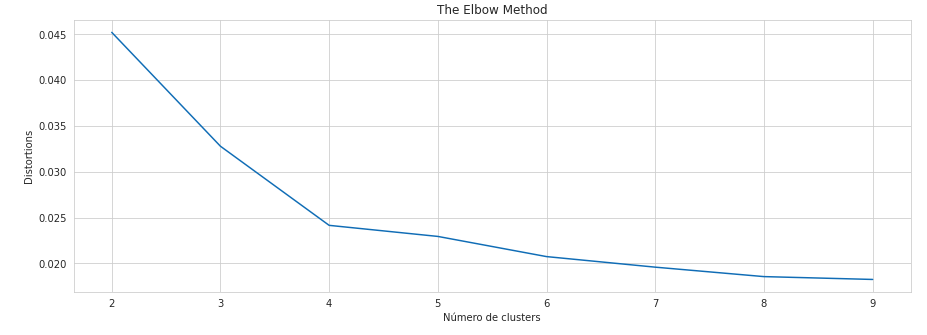
\includegraphics[width=1\linewidth]{img/elbow6}
	\caption{}
	\label{fig:elbow6}
\end{figure}

y deducimos así que el número de clusters óptimo aquí es de 4. Ejecutamos entonces el algoritmo llamando a la función \mintinline{python}{k_means} con k=4:
\begin{minted}{python}
	result3=k_means(data_caso3,4)
\end{minted}

y obtenemos la siguiente salida:
\begin{minted}{python}
	Silhouette: 0.718011
	Calinsky: 7644.620592
\end{minted}
\textbf{Análisis de los clusters obtenidos}

Para analizar los clusters que obtenemos en este caso de estudio con el algoritmo de K-means, tenemos en cuenta las mismas visualizaciones que hemos venido usando hasta ahora:


\begin{figure}[H]
	\centering
	\caption[]{Countplot}
	\label{fig:count6}
	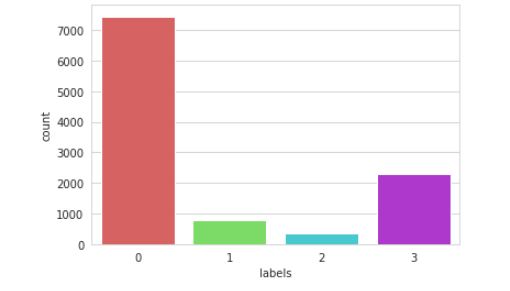
\includegraphics[width=0.9\linewidth]{img/count6}
\end{figure}
\begin{figure}[H]
	\centering
	\caption[]{Mapa de calor}
	\label{fig:heatmap6}
	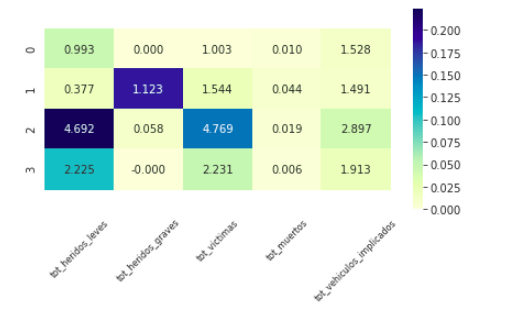
\includegraphics[width=0.9\linewidth]{img/heatmap6}
\end{figure}
\begin{figure}[H]
	\centering
	\caption[]{Imagen pairplot}
	\label{fig:pairplot6}
	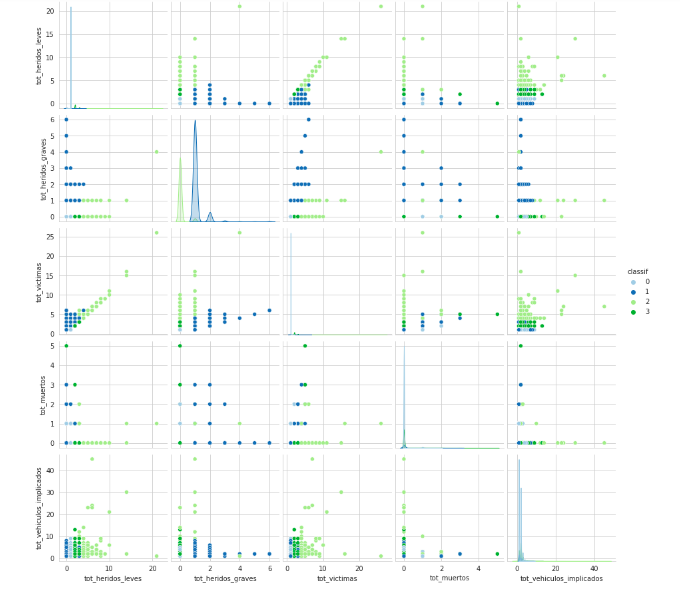
\includegraphics[width=1\linewidth]{img/pairplot6}
\end{figure}
\begin{figure}[H]
	\centering
	\caption[]{Diagramas de cajas}
	\label{fig:cajas6}
	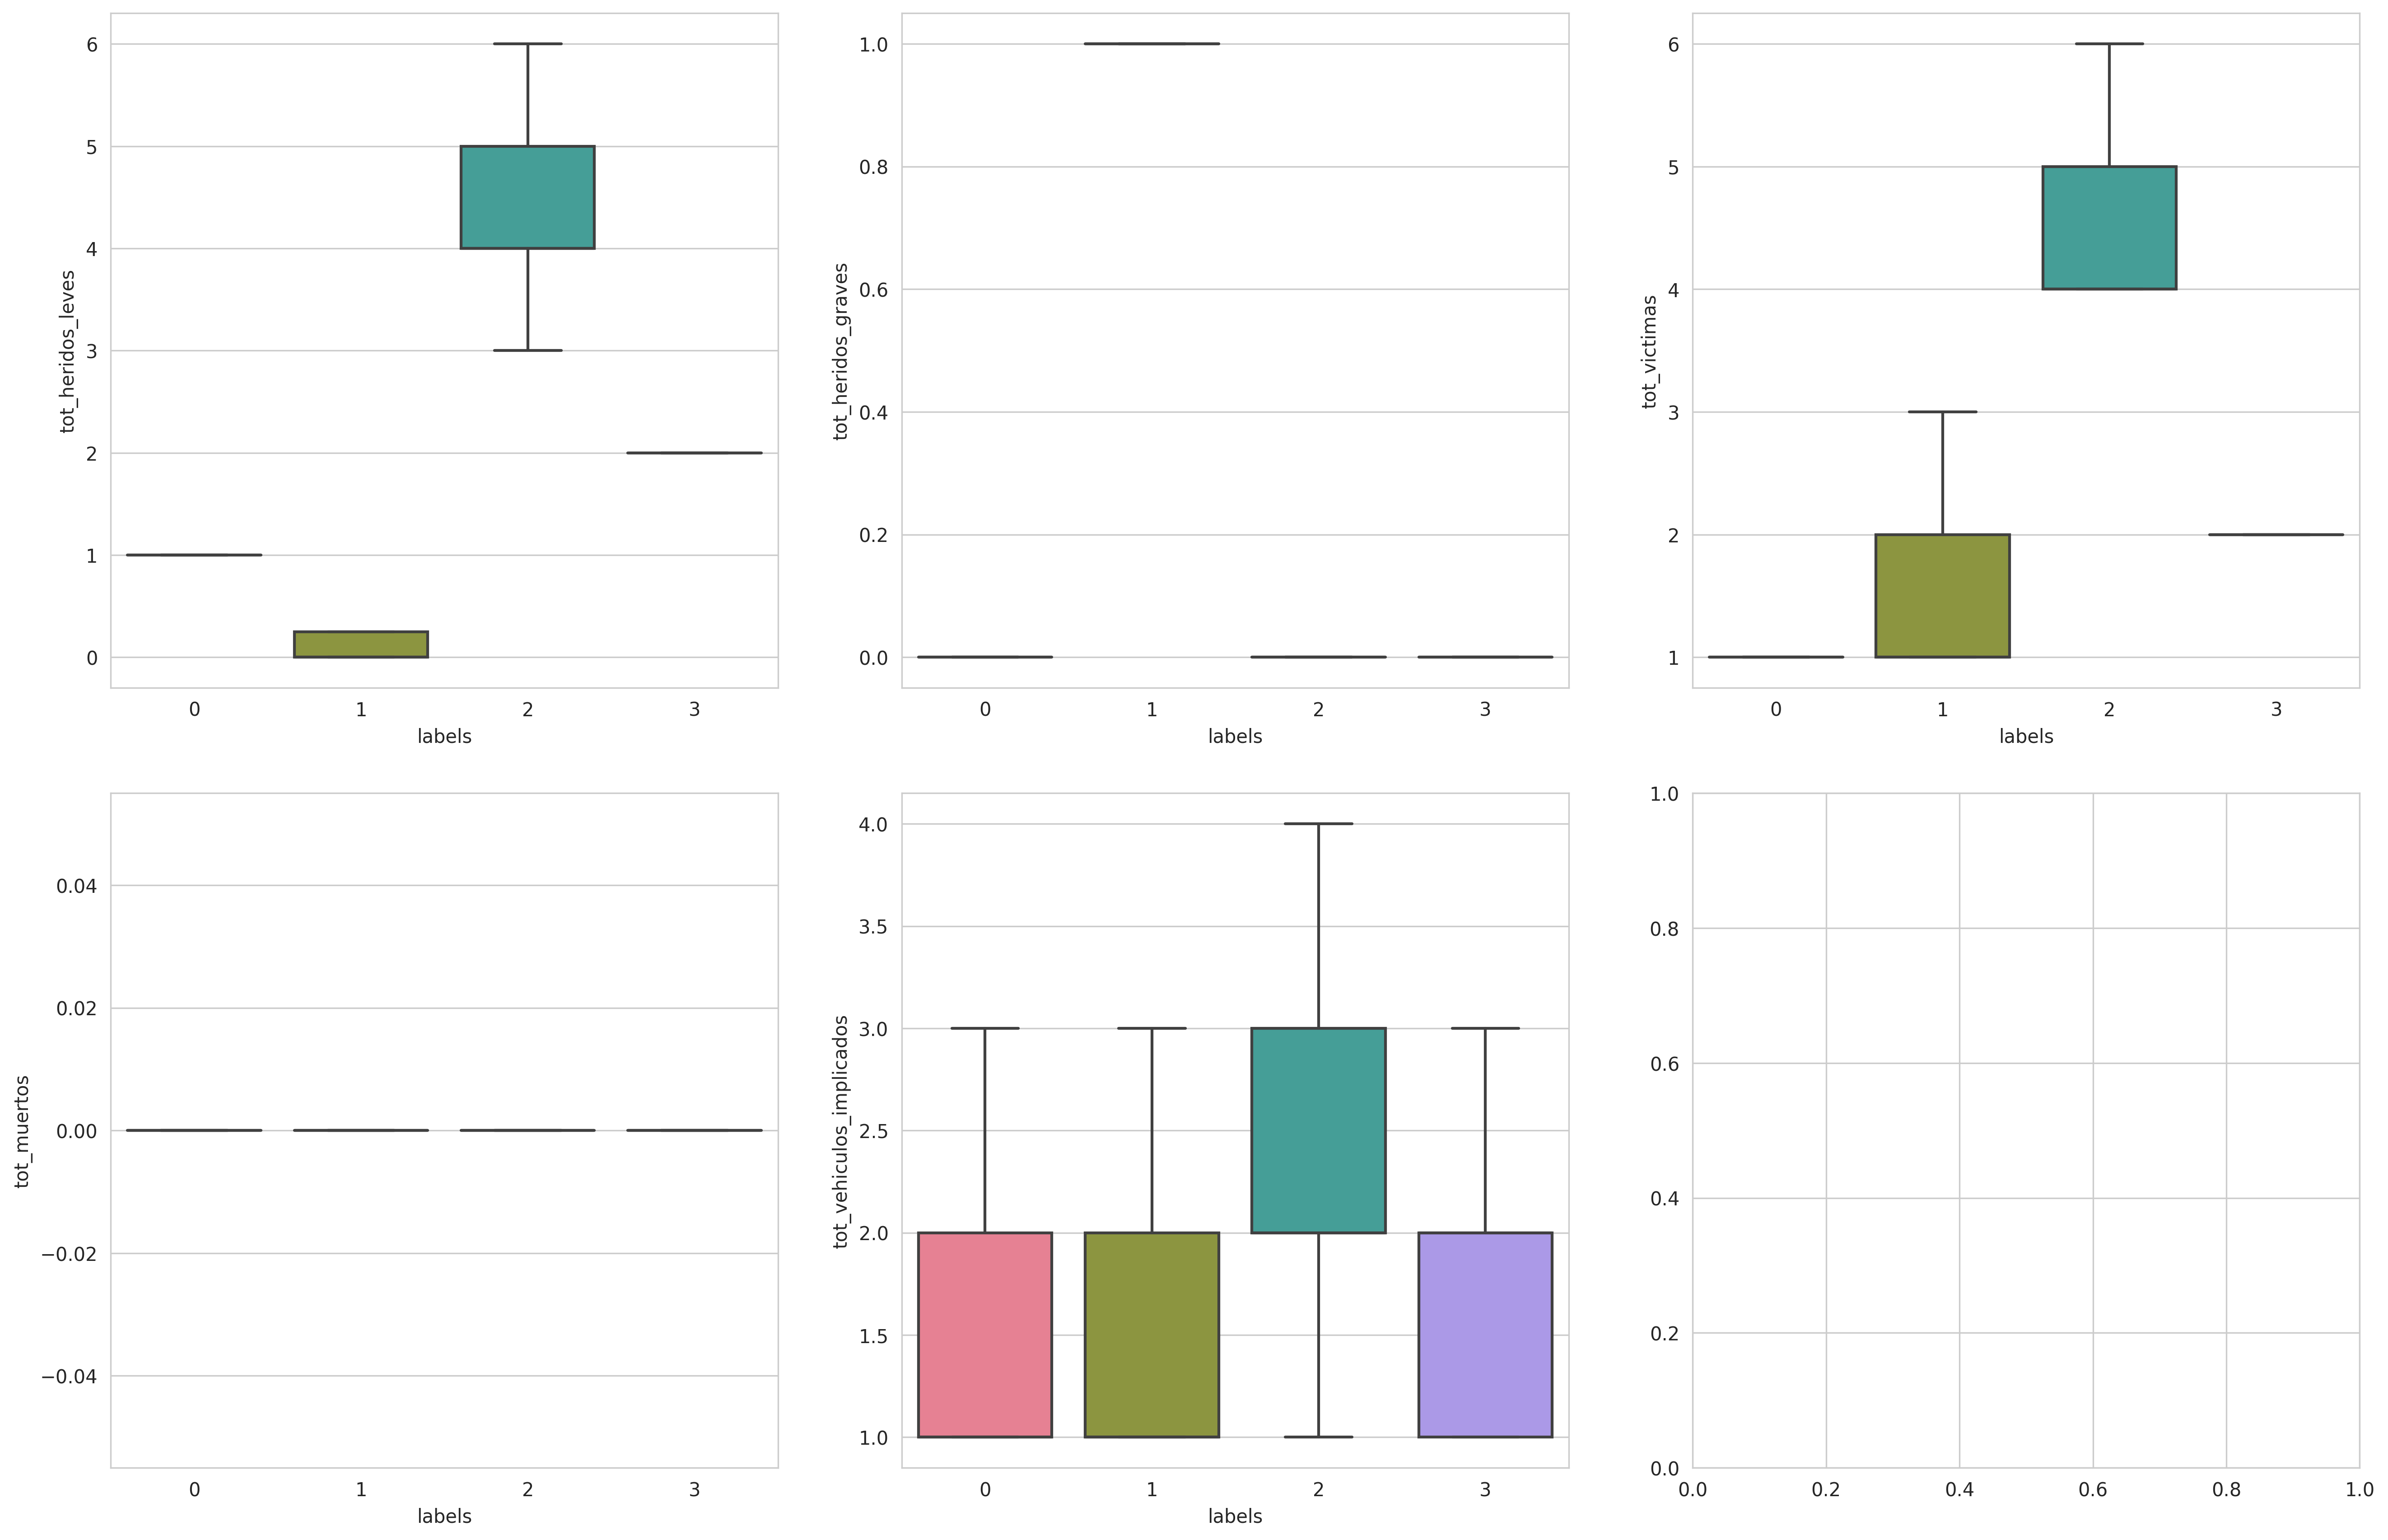
\includegraphics[width=1.1\linewidth]{img/cajas6}
\end{figure}

Los aspectos más destacables de los clusters obtenidos son los siguientes:
\begin{itemize}
	\item El número de muertos es prácticamente 0 en todos los grupos, por lo que, salvo casos atípicos, no hay fallecidos en los accidentes considerados.
	\item En cuanto a los vehículos implicados, varían entre 1 y 3 en los clusters de mayor tamaño (0, 1 y 3), siendo 1 o 2 con más frecuencia. El cluster número 2, que es el más pequeño, contiene accidentes en los que intervienen un número mayor de vehículos, variando entre 1 y 4, y siendo 2 o 3  vehículos lo más común dentro de este grupo.
	\item La mayor parte de los datos quedan recogidos en el \underline{clúster número 0}, el cual está caracterizado porque el número de heridos leves en sus instancias es 1 y el número de heridos graves y muertos es nulo. 
	\item El siguiente cluster de mayor tamaño, que recoge en torno a 2000 datos, es el \underline{clúster número 3}. Este incluye los accidentes en los que el número de heridos leves es de 2.
	\item Encontramos algunos accidentes, menos de 1000, en los que resulta un herido grave y, en algunos casos, también alguno leve (\underline{clúster 1}).
	\item Una minoría de los casos, agrupados en el \underline{cluster 2}, que tiene un tamaño de menos de 500 datos, presenta un mayor número de heridos leves como consecuencia de un mayor número de vehículos implicados. El número de heridos varía entre 3 y 6, aunque en la mitad de los accidentes que se recogen aquí el número de heridos leves es de 4 o 5. 
\end{itemize}
\newpage
\subsection{Interpretación de la segmentación. \\ Comparación con el caso de estudio 2}

Intentamos ahora interpretar la segmentación obtenida en este caso de estudio así como las diferencias presentes entre estos resultados y los que obtuvimos en el caso de estudio 2. 

Como viene ocurriendo en los dos casos de estudio analizados, lo más común es que en los datos sólo aparezcan uno o dos heridos leves como resultado de un accidente en el que intervienen 1, 2 o, a lo sumo, 3 vehículos, sin heridos graves o muertos. Ya comentamos al principio que esto es lógico, pues en la mayoría de los accidentes que ocurren normalmente no hay heridos de gravedad o muertos, solo en una pequeña proporción de los mismos, de ahí que aquí también obtengamos que este tipo de accidentes son los menos frecuentes. 

Sin embargo, si nos fijamos en los diagramas de cajas de la variable \textit{total de vehículos implicados} obtenidos tras aplicar el algoritmo DBSCAN, el cual detecta bien los outliers, en el caso de estudio 2 nos damos cuenta de que no hay accidentes (salvo en los outliers) en los que intervengan más de 3 vehículos y en los que intervienen 3 vehículos son poco frecuentes. En este caso de estudio, por lo contrario, sí que obtenemos un cluster con varias instancias (algunas centenas) que recoge algunos datos con más de 3 vehículos implicados y en muchos de los cuales intervienen 3 vehículos. Esto puede ser debido a que, aunque la calzada siga estando en este nuevo caso de estudio en condiciones adversas (nevada, helada, mojada), al ser de día o haber suficiente iluminación, hay más movilidad de vehículos y personas, de modo que el tráfico es más elevado que si fuera de noche, en zonas con iluminación insuficiente, lo cual implica que cuando se produce un accidente es más probable que más vehículos se vean involucrados. Además, a mayor movilidad de personas, más usual es que haya varios pasajeros en un mismo vehículo. Este hecho, junto con una mayor probabilidad de que haya más vehículos implicados, propicia que resulte un mayor número de heridos leves tras un accidente, de ahí que aquí tengamos un cluster con algunas centenas de instancias que contiene datos en los que el número de heridos leves es 4 y 5 normalmente, o incluso 6 en algunos casos. En el caso de estudio 2, los clusters con un número más elevado de heridos leves tenían un tamaño ínfimo comparado con el tamaño del cluster que en el nuevo caso de estudio aparece. 

Por otro lado, hemos comprobado que en el caso de estudio 3 no hay ningún grupo en que se recojan accidentes con algún fallecido, sino que estos accidentes son outliers y no forman parte de ningún cluster concreto. Por el contrario, en el caso de estudio 2, sí que encontrábamos un grupo con accidentes en los que alguna persona fallecía. Esto nos dice que bajo condiciones de escasa iluminación es más probable que los accidentes tengan una mayor gravedad, tanto que alguien puede incluso fallecer en estos casos. 

Finalmente, en los dos casos de estudio comparados, aparece un grupo de tamaño considerable en el que se recogen los accidentes en los que resulta algún herido grave. Es decir, aunque cuando la iluminación es suficiente es poco probable que alguien muera en un accidente, sí que es frecuente que se produzcan heridos graves, siguen ocurriendo accidentes graves pero sin fallecidos. Como ya hemos dicho, esto es lógico pues estamos considerando situaciones en las que la calzada se encuentra resbaladiza y en un estado peligroso para la circulación, de manera que, aunque la iluminación cambie, es común que resulten heridos graves en los accidentes bajo estas condiciones. 

\begin{thebibliography}{9}
\bibitem{1} 	
\url{https://www.kaggle.com/vjchoudhary7/kmeans-clustering-in-customer-segmentation}

\bibitem{2} 
\url{https://scikit-learn.org/stable/modules/clustering.html}

\bibitem{3} 
\url{https://scikit-learn.org/stable/modules/generated/sklearn.cluster.KMeans.html}

\bibitem{4} 
\url{https://www.geeksforgeeks.org/elbow-method-for-optimal-value-of-k-in-kmeans/}

\bibitem{5} 
\url{https://en.wikipedia.org/wiki/Elbow_method_(clustering)}
\bibitem{6} 
\url{https://scikit-learn.org/stable/modules/clustering.html#hierarchical-clustering}
\bibitem{7} 
\url{https://scikit-learn.org/stable/modules/generated/sklearn.cluster.AgglomerativeClustering.html#sklearn.cluster.AgglomerativeClustering}
\bibitem{8} 
\url{https://www.sigmamagic.com/blogs/hierarchical-clustering/}
\bibitem{9} 
\url{https://sites.google.com/site/dataclusteringalgorithms/hierarchical-clustering-algorithm}
\bibitem{10} 
\url{https://scikit-learn.org/stable/modules/generated/sklearn.cluster.DBSCAN.html#sklearn.cluster.DBSCAN}
\bibitem{11} 
\url{https://towardsdatascience.com/k-means-vs-dbscan-clustering-49f8e627de27}
\bibitem{12} 
\url{https://scikit-learn.org/stable/modules/clustering.html#dbscan}
\bibitem{13}
\url{https://medium.com/devtorq/dbscan-a-walkthrough-of-a-density-based-clustering
-method-b5e74ca9fcfa}

\end{thebibliography}
\end{document}
